\documentclass[a4paper,openany, 12pt]{book}
%Journal names
\newcommand{\apj}{ApJ}
\newcommand{\apjl}{ApJ}
\newcommand{\apjs}{ApJS}
\newcommand{\aap}{A\&A}
\newcommand{\aaps}{A\&AS}
\newcommand{\aj}{AJ}
\newcommand{\mnras}{MNRAS}
\newcommand{\pasj}{PASJ}
\newcommand{\physrep}{Physics Reports}
\newcommand{\prd}{PRD}
\newcommand{\prl}{PRL}
\newcommand{\nat}{Nature}
\newcommand{\araa}{ARAA}
\newcommand{\jcap}{JCAP}
\newcommand{\pasa}{PASA}
\newcommand{\pasp}{PASP}
\newcommand{\procspie}{Proceedings of SPIE}




\usepackage[text={15.5cm,23cm},centering]{geometry}

\newcommand\savemathcal[1]{%
  \expandafter\newsavebox\csname mc#1content\endcsname%
  \expandafter\savebox\csname mc#1content\endcsname{$\mathcal{#1}$}%
  \expandafter\newcommand\csname mc#1\endcsname{%
    \expandafter\usebox\expandafter{\csname mc#1content\endcsname}}%
}
\newcommand\altmathcal[1]{\csname mc#1\endcsname}
\savemathcal{Z}
\savemathcal{B}

\usepackage{mathptmx}
\usepackage{graphicx}
\usepackage{chapterbib} %remember to bibtex each chapter before final compilation
\usepackage{subfigure}
\usepackage{color}
\usepackage{amsmath}
\usepackage{amssymb}
\usepackage[colorlinks=true, linkcolor=blue]{hyperref}
\urlstyle{same}

\usepackage[english]{babel}  %For Vibor's institution characters

\newcommand{\chapterauthor}[1]{\textsc{#1}\section*{}}  % Only needed for edited/contributed books

%defines some roman math characters
\newcommand{\rmd}{\ensuremath{\mathrm{d}}}
\newcommand{\rme}{\ensuremath{\mathrm{e}}}
\newcommand{\rmi}{\ensuremath{\mathrm{i}}}

% Added by JM to get subsub sections numbered
\setcounter{secnumdepth}{4}


\title{The cosmic 21-cm revolution: charting the first billion years of our Universe}
\author{Andrei Mesinger}




\begin{document}
\frontmatter
\maketitle
\tableofcontents

\chapter*{Preface}
\label{Preface}


This set of files can be used to create your typescript in \LaTeX. You can add packages as necessary.

Remember that references need to be at the chapter level and you may find the package \href{http://www.ctan.org/pkg/chapterbib}{chapterbib} useful for this.
\chapter*{About the Author}


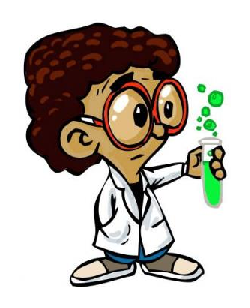
\includegraphics{Mesinger/Author}

Remenber to include a brief biography of the Authors or Editors, including a photo.


\chapter*{Contributors}
 
%Only needed for edited collections. Include all contributors, listed alphabetically by surname, along with their affiliation.  


%\raggedright
{\parskip=12pt

\noindent\textbf{Vibor Jeli\'c}\\
Ru{\dj}er Bo\v{s}kovi\'{c} Institute\\
Zagreb, Croatia 

\noindent\textbf{Peter Jones}\\
Department of Physics\\
University of New England\\
Acadia, Maine, USA

\noindent\textbf{Simon Smith}\\
Department of Electrical Engineering\\
University of Oxbridge, 
Camford, USA

\noindent\textbf{Cathryn M. Trott}\\
International Centre for Radio Astronomy Research\\
Curtin University, Bentley WA, Australia

}
 %only needed for edited books


\mainmatter


\chapter{Theoretical Framework: The Fundamentals of the 21-cm Line}

\begin{bf}
  \author{Steven R. Furlanetto}\\

  Abstract\\

We review some of the fundamental physics necessary for computing the highly-redshifted spin-flip background. We first discuss the radiative transfer of the 21-cm line and define the crucial quantities of interest. We then review the processes that set the spin temperature of the transition, with a particular focus on Wouthuysen-Field coupling, which is likely to be the most important process during and after the Cosmic Dawn. Finally, we discuss processes that heat the intergalactic medium during the Cosmic Dawn, including the scattering of Lyman-$\alpha$, cosmic microwave background, and X-ray photons.
\end{bf}

\section{Radiative Transfer of the 21-cm Line} \label{rt-21cm}

Consider a spectral line labeled by 0 (the lower level) and 1 (the upper level). The radiative transfer equation for the specific intensity $I_\nu$ of photons at the relevant frequency is
\begin{equation}
{dI_\nu\over d\ell}={\phi(\nu) h\nu\over 4\pi}\left[n_1 A_{10} -
\left(n_0 B_{01} -n_1 B_{10}\right)I_\nu\right],
\label{rad}
\end{equation}
where $d\ell$ is a proper path length element, $\phi(\nu)$ is the line profile function, $n_i$
denotes the number density of atoms at the different levels, and $A_{ij}$ and $B_{ij}$ are the Einstein coefficients for the relevant transition (here $i$ and $j$ the initial and final states, respectively). For the 21-cm line, the line frequency is $\nu_{21} = 1420.4057$~MHz. The Einstein relations associate the radiative transition rates via $B_{10}=(g_0/g_1)B_{01}$ and $B_{10}=A_{10}(c^2/2 h\nu^3)$, where $g$ is the spin degeneracy factor of each state. For the 21-cm transition, $A_{10}=2.85\times 10^{-15} \ {\rm s^{-1}}$ and $g_1/g_0=3$.

The relative populations of hydrogen atoms in the two spin states determine the {\bf spin temperature}, $T_S$, through the relation
\begin{equation}
\left({n_1\over n_0}\right)=\left({g_1 \over g_0}\right)
\exp\left\{ {-T_*\over T_S}\right\}, 
\end{equation}
where $T_* \equiv E_{10} /k_B=68$~mK is equivalent to the transition energy $E_{10}$. In almost all physically plausible situations,  $T_\star$ is much smaller than any other temperature, including $T_S$, so all the exponentials in temperature can be Taylor expanded to leading order with high accuracy. Note, however, that $T_S$ implicitly assumes that the level populations can be described by a single temperature -- independent of each atom's velocity. In detail, velocity-dependent effects must be considered in certain circumstances \cite{hirata07}.

It is conventional to replace $I_{\nu}$ by the equivalent {\bf brightness temperature}, $T_b(\nu)$, required of a blackbody radiator (with spectrum $B_{\nu}$) such that $I_{\nu}=B_{\nu}(T_b)$. In the low frequency regime relevant to the 21 cm line, the Rayleigh-Jeans formula is an excellent approximation to the Planck curve, so $T_b(\nu)\approx I_{\nu} \, c^2/2k_B{\nu}^2$.

In this limit, the equation of radiative transfer  along a line of sight through a cloud of uniform excitation temperature $T_S$ becomes
\begin{equation}
T_b'(\nu) = T_{S}(1-e^{-\tau_{\nu}})+T_R'(\nu)e^{-\tau_{\nu}}
\label{eq:rad_trans}
\end{equation}
where $T_b'(\nu)$ is the emergent brightness measured at the cloud and at redshift $z$, the {\bf optical depth}  $\tau_\nu \equiv \int d s \, \alpha_{\nu}$ is the integral of the absorption coefficient ($\alpha_{\nu}$)  along the ray through the cloud, $T_R'$ is the brightness of the background radiation field incident on the cloud along the ray, and $s$ is the proper distance. Because of the cosmological redshift, for the 21-cm transition an observer will measure an apparent brightness at the Earth of $T_b(\nu) = T_b'(\nu_{21})/(1+z)$, where the observed frequency is $\nu=\nu_{21}/(1+z)$. Henceforth we will work in terms of these observed quantities.

The absorption coefficient is related to the Einstein coefficients via
\begin{equation}
\alpha = \phi(\nu) {h \nu \over 4 \pi} (n_0 B_{01} - n_1 B_{10}).
\end{equation}
Because all astrophysical  applications have $T_S \gg T_*$, approximately three of four atoms find themselves in the excited state ($n_0 \approx n_1/3$).  As a result, the stimulated emission correction represented by the first term is significant.  

The fundamental observable quantity is the change in brightness temperature induced by the 21-cm line by a patch of the intergalactic medium (IGM), relative to the incident radiation field. In most models that incident field is simply the cosmic microwave background, although if other sources create a low-frequency radio background at very high redshifts, or if there is a particular source behind the IGM patch along the line of sight from the observer, a larger radio background may exist.

Consider photons incident on the patch from this background. If any redshift into resonance with the 21-cm line, they can interact with the cloud -- but only for a short time, as they will redshift out of resonance as the Universe continues to expand. Thus the Hubble expansion rate sets an effective path length through the cloud, simply equal to the distance the photon travels while it remains within the line profile. The total absorption can be calculated by integrating the IGM density across this interval, in an exactly analogous procedure to the calculation of the Gunn-Peterson Lyman-$\alpha$ optical depth \cite{field59-obs, gunn65, scheuer65}. The result is
\begin{eqnarray}
\tau_{10} & = & \frac{3}{32 \pi} \, \frac{h c^3 A_{10}}{k_B T_S \nu_{10}^2} \, \frac{x_{\rm HI} n_{\rm H}}{(1+z) \, (d v_\parallel/d r_\parallel)}  \label{eq:optdepthcosmo} \\
 & \approx  & 0.0092 \, (1+\delta) \, (1+z)^{3/2}\, \frac{x_{\rm HI}}{T_S} \, \left[ \frac{H(z)/(1+z)}{d v_\parallel/d r_\parallel} \right],
\label{optdepthcosmo-approx}
\end{eqnarray}
where $n_H$ is the hydrogen number density, $x_{\rm HI}$ is the neutral fraction, $dv_\parallel/dr_\parallel$ is the velocity gradient along the line of sight (here scaled to the Hubble flow). In the second part,$T_S$ is in Kelvins, and we have scaled the density to the mean value by writing $n_H = \bar{n}_H^0 (1+z)^3 (1 + \delta)$, where $\bar{n}_H^0$ is the mean comoving density today.

In most circumstances, the CMB provides the background radiation source, for which with temperature $T_\gamma(z)$. Then $T_R' = T_{\gamma}(z)$, so that  we are observing the contrast between high-redshift hydrogen clouds and the CMB.   Because the optical depth is so small, we can then expand the exponentials in equation~(\ref{eq:rad_trans}), and
\begin{eqnarray}
& T_b(\nu) & \approx \frac{T_S-T_{\gamma}(z)}{1+z}\;\tau_{\nu_0} 
\label{eq:dtbone} \\
& \approx & 9\;x_{\rm HI}(1+\delta) \, (1+z)^{1/2}\, \left[1-\frac{T_{\gamma}(z)}{T_S}\right] \, \left[ \frac{H(z)/(1+z)}{d v_\parallel/d r_\parallel} \right] \ \mbox{mK}.
\label{eq:dtb}
\end{eqnarray}
Thus $T_b < 0$ if $T_S < T_{\gamma}$, yielding an absorption signal; otherwise it appears in emission relative to the CMB. Both regimes are likely important for the high-$z$ Universe. Note that $T_b$ saturates if $T_S \gg T_{\gamma}$, but the absorption can become arbitrarily large if $T_S \ll T_{\gamma}$.  The observability of the 21 cm transition therefore hinges on the spin temperature; we will next describe the mechanisms that control that factor.

\section{The Spin Temperature} \label{spin-temp}

Three competing processes determine $T_S$: {\it (i)} absorption of CMB photons (as well as stimulated emission); {\it (ii)} collisions with other particles; and{\it (iii)} scattering of UV photons.  In the presence of the CMB
alone, the spin states reach thermal equilibrium ($T_S=T_{\gamma}$) on a time-scale of $\sim T_*/(T_\gamma A_{10}) = 3 \times 10^5 (1+z)^{-1}$ yr -- much shorter than the age of the Universe at all redshifts after cosmological recombination, indicating that CMB coupling establishes itself rapidly. Indeed all the relevant processes adjust on very short timescales (compared to the Hubble time) so equilibrium is an excellent approximation.

However, the other two processes break this coupling. We let $C_{10}$ and $P_{10}$ be the de-excitation rates (per atom) from collisions and UV scattering, respectively.  We also let $C_{01}$ and $P_{01}$ be the
corresponding excitation rates.  In equilibrium, the spin temperature is then
determined by
\begin{equation}
n_1 \left( C_{10} + P_{10} + A_{10} + B_{10} I_{\rm CMB} \right) = n_0 \left( C_{01} + P_{01} + B_{01} I_{\rm CMB} \right),
\label{eq:detbal}
\end{equation}
where $I_{\rm CMB}$ is the specific intensity of CMB photons at $\nu_{21}$.  With the Rayleigh-Jeans approximation, equation (\ref{eq:detbal}) can be rewritten as
\begin{equation}
T_S^{-1} = \frac{T_\gamma^{-1} + x_c T_K^{-1} + x_\alpha T_c^{-1}}{1 + x_c + x_\alpha},
\label{eq:xdefn}
\end{equation}
where $x_c$ and $x_\alpha$ are coupling coefficients for collisions and UV scattering, respectively, and $T_K$ is the gas kinetic temperature.  Here we have used the principle of detailed balance through the relation
\begin{equation}
\frac{C_{01}}{C_{10}} = \frac{g_1}{g_0} e^{-T_\star/T_K} \approx 3 \left( 1 - \frac{T_\star}{T_K} \right).
\label{eq:c01db}
\end{equation}
We have also \emph{defined} the effective color temperature of the UV radiation field $T_c$ via
\begin{equation}
\frac{P_{01}}{P_{10}} \equiv 3 \left( 1 - \frac{T_\star}{T_c} \right).
\label{eq:tcolor}
\end{equation}
In the limit in which $T_c \rightarrow T_K$ (usually a good approximation), equation~(\ref{eq:xdefn}) may be written 
\begin{equation}
1 - \frac{T_\gamma}{T_S} = \frac{x_c + x_\alpha}{1 + x_c + x_\alpha} \, \left( 1 - \frac{T_\gamma}{T_K} \right).
\label{eq:xdefn-tfac}
\end{equation}

We must now calculate $x_c$,  $x_\alpha$, and $T_c$, which we shall do in the next subsections.

\subsection{Collisional Coupling} \label{coll}

We will first consider collisional excitation and de-excitation of the hyperfine levels, which become important in dense gas.  The coupling coefficient for collisions with species $i$ is
\begin{equation}
x_c^i \equiv  \frac{C_{10}^i}{A_{10}} \, \frac{T_\star}{T_\gamma} = \frac{n_i \, \kappa_{10}^i}{A_{10}} \, \frac{T_\star}{T_\gamma},
\label{eq:xcdefn}
\end{equation}
where $\kappa_{10}^i$ is the rate coefficient for collisional spin de-excitation in collisions (with units of cm$^3$ s$^{-1}$).  The total $x_c$ is the sum over all relevant species $i$, including collisions with (1) neutral hydrogen atoms, (2) free electrons, and (3) protons.  

These rate coefficients can be calculated by the quantum mechanical cross sections of the relevant processes \cite{zygelman05, furl07-electron, furl07-proton}. We will not list them in detail but show the rates in Figure~\ref{fig:collrates}.  Although the atomic cross-section is small, in the unperturbed IGM collisions between neutral hydrogen atoms nearly always dominate these rates because the ionized fraction is small.  Free electrons can be important in partially ionized gas; collisions with protons are only important at the lowest temperatures.

%%%%%: FIGURE: Collision rates
\begin{figure}[]
\begin{center}
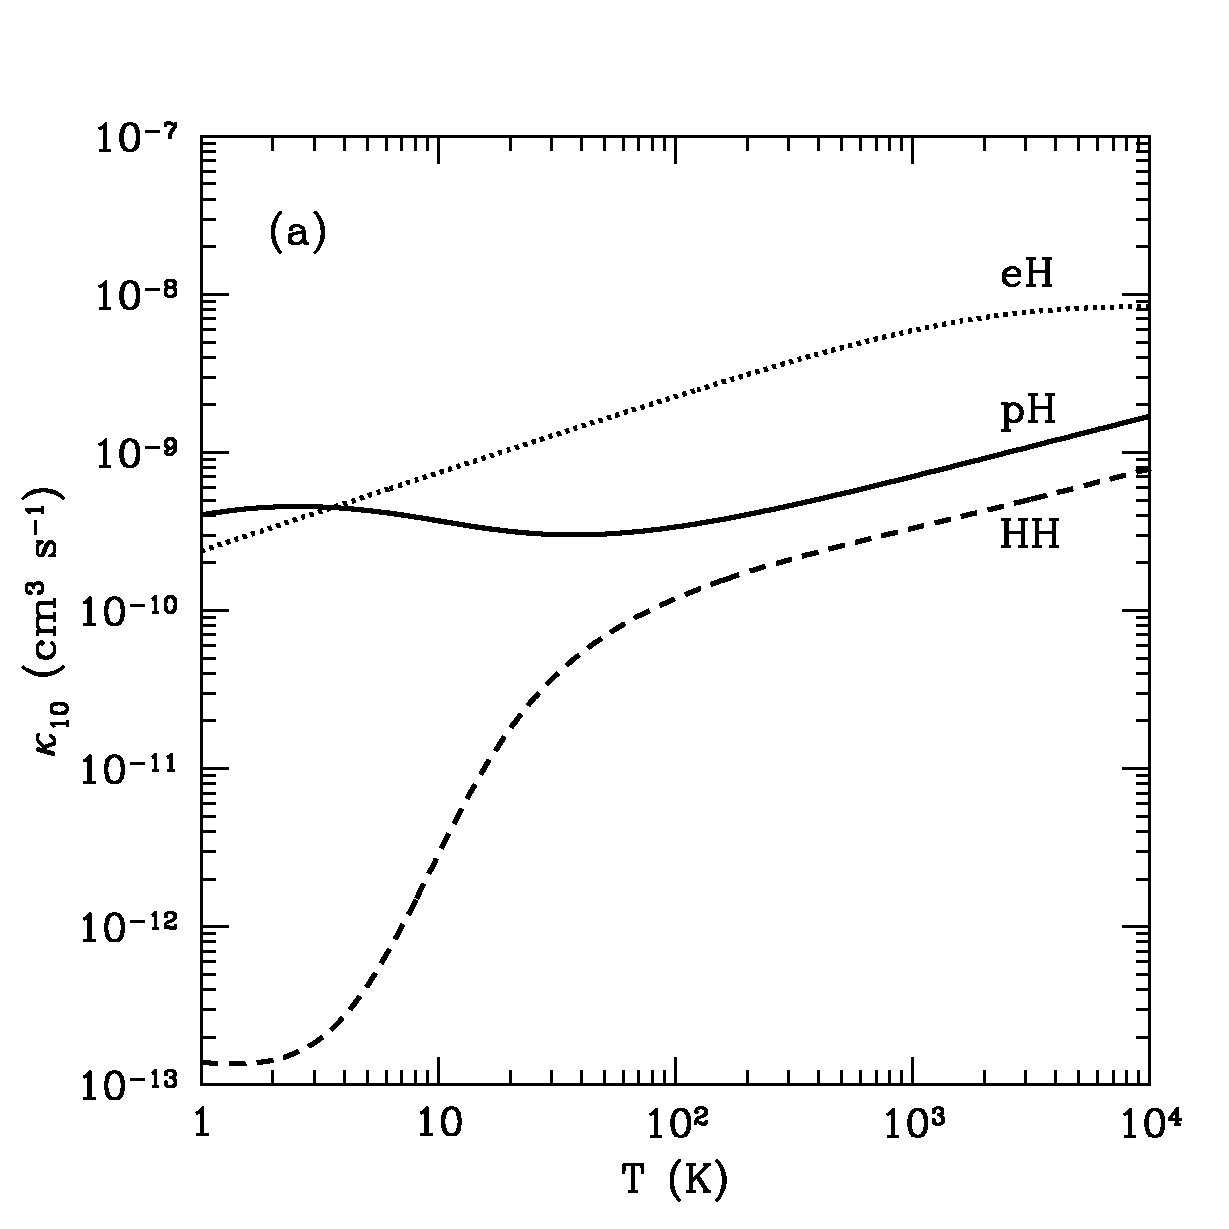
\includegraphics[width=0.5\textwidth]{Furlanetto/figure2-1}
\end{center}
\caption{De-excitation rate coefficients for H-H collisions (dashed
line), H-e$^-$ collisions (dotted line), and H-p collisions (solid
line).  Note that the net rates are also proportional to the densities
of the individual species, so H-H collisions still dominate in a
weakly-ionized medium. From \cite{furl07-proton}.}
\label{fig:collrates}
\end{figure}

Given the densities relevant to the IGM, collisional coupling is quite weak in a nearly neutral, cold medium.  Thus, the local density must be large in order for this process to effectively fix $T_S$. A convenient estimate of their
importance is the critical overdensity, $\delta_{\rm coll}$, at which
$x_c=1$ for H--H collisions:
\begin{equation}
1 + \delta_{\rm coll} = 0.99 \, \left[ \frac{\kappa_{10}(88 \ \mbox{K})}{\kappa_{10}(T_K)} \right] \, \left( \frac{0.023}{\Omega_b
    h^2} \right) \, \left( \frac{70}{1+z} \right)^2,
\label{eq:dcoll}
\end{equation}
where 88~K is the expected IGM temperature at $1+z=70$.\footnote{Note that this is \emph{smaller} than the CMB temperature at this time, because the IGM gas cools faster (due to adiabatic expansion) once Compton scattering becomes inefficient at $z \sim 150$.}  In the standard picture, at redshifts $z < 70$, $x_c \ll 1$ and $T_S \rightarrow T_{\gamma}$; by $z \sim 30$ the IGM essentially becomes invisible.  However, $\kappa_{10}$ is extremely sensitive to $T_K$ in this low-temperature regime.  If the Universe is somehow heated above the fiducial value, the threshold density can remain modest: $\delta_{\rm coll} \approx 1$ at $z=40$ if $T_K=300$~K.

\subsection{The Wouthuysen-Field Effect} \label{wf}

We must therefore appeal to a different mechanism to render the 21-cm transition visible during the era of the first galaxies.  This is known as the {\bf Wouthuysen-Field mechanism} (named after the Dutch physicist Siegfried
Wouthuysen and Harvard astrophysicist George Field who first explored it \cite{wouthuysen52, field58}). Figure~\ref{fig:wf} illustrates the effect. This shows the hyperfine sub-levels of the $1S$ and $2P$ states of HI and the permitted transitions between them.  Suppose a hydrogen atom in the hyperfine singlet state absorbs a Lyman-$\alpha$ photon.  The electric dipole selection rules allow $\Delta F=0,1$ except that $F=0 \rightarrow 0$ is prohibited (here $F$ is the total angular momentum of the atom).  Thus the atom must jump to either of the central $2P$ states.  However, these same rules now allow electrons in either of these excited states to decay to the $_1S_{1/2}$ triplet level.\footnote{Here we use the notation $_F L_J$, where $L$ and $J$ are the orbital and total angular momentum of the electron.}  Thus, atoms can change hyperfine states through the absorption and spontaneous re-emission of a Lyman-$\alpha$ photon (or indeed any Lyman-series photon; see below).

%%%%%: FIGURE: W-F levels
\begin{figure}[]
\begin{center}
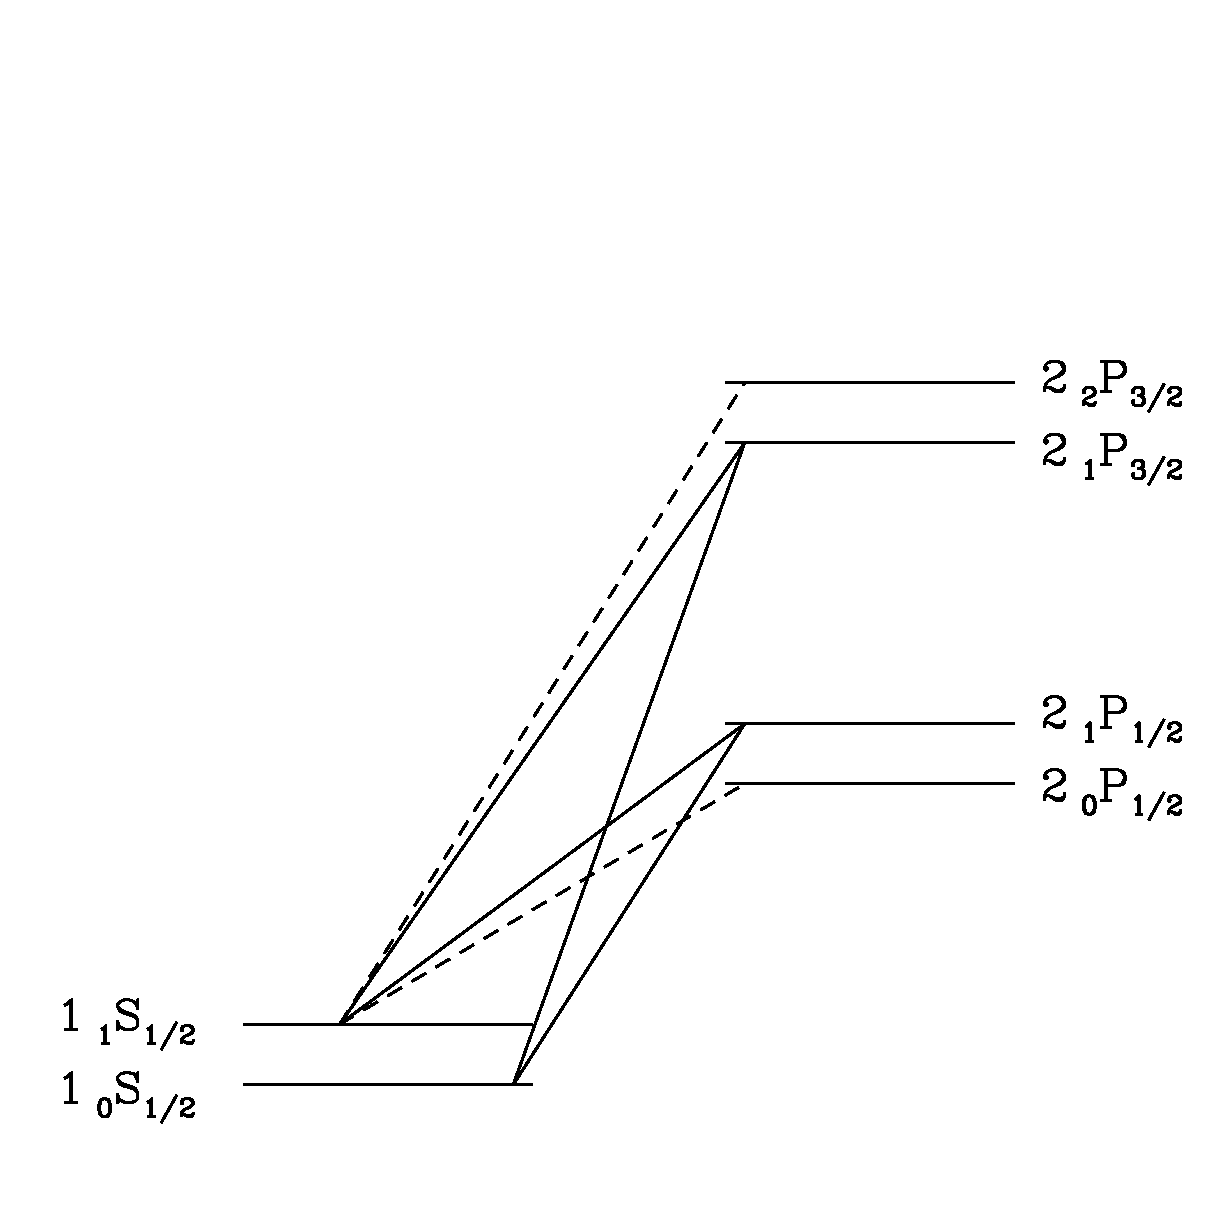
\includegraphics[width=0.6\textwidth]{Furlanetto/figure2-2}
\end{center}
\caption{Level diagram illustrating the Wouthuysen-Field effect.  We show the hyperfine splittings of the $1S$ and $2P$ levels.  The solid lines label transitions that can mix the ground state hyperfine levels, while the dashed lines label complementary allowed transitions that do not participate in mixing.  From \cite{pritchard06}.}
\label{fig:wf}
\end{figure}

The Wouthuysen-Field coupling rate depends ultimately on the total rate (per atom) at which Lyman-$\alpha$ photons scattered through the gas,
\begin{equation}
P_\alpha = 4 \pi \sigma_0 \int d \nu \, J_\nu(\nu) \phi_\alpha(\nu),
\label{eq:palpha}
\end{equation}
where $\sigma_\nu \equiv \sigma_0 \phi_\alpha(\nu)$ is the local Lyman-$\alpha$ absorption cross section, $\sigma_0 \equiv (\pi \, e^2/m_e \, c) f_{\alpha}$, $f_\alpha=0.4162$ is the oscillator strength of the Lyman-$\alpha$ transition, $\phi_\alpha(\nu)$ is the Lyman-$\alpha$ absorption profile, and $J_\nu$ is the angle-averaged specific intensity of the background radiation field.\footnote{By convention, we use the specific intensity in units of photons cm$^{-2}$ Hz$^{-1}$ s$^{-1}$ sr$^{-1}$ here, which is conserved during the expansion of the Universe (whereas a definition in terms of energy instead of photon number is subject to redshifting).}   

Transitions to higher Lyman-$n$ levels have similar effects \cite{hirata06, pritchard06}. Suppose that a UV photon redshifts into the Lyman-$n$ resonance as it travels through the IGM.  After absorption, it can either scatter (by the electron decaying directly to the ground state) or cascade through a series of intermediate levels and produce a sequence of photons.  The direct decay probability for any level is $\sim 0.8$, so a Lyman-$n$ photon will typically scatter $N_{\rm scatt} \approx (1-P_{nP\rightarrow1S})^{-1} \sim 5$ times before instead initiating a decay cascade.  In contrast, Lyman-$\alpha$ photons scatter hundreds of thousands of times before being destroyed, usually be redshifting all the way across the (very wide) Lyman-$\alpha$ profile.  As a result, coupling from the direct scattering of Lyman-$n$ photons is suppressed compared to Lyman-$\alpha$ by a large factor.

However, Lyman-$n$ photons can still be important because of their cascade products, as shown in Figure~\ref{fig:lygamma}.  Following Lyman-$\beta$ absorption, the only permitted decays are to the ground state (regenerating a Lyman-$\beta$ photon and starting the process again) or to the $2S$ level.  The H$\alpha$ photon produced in the $3P \rightarrow 2S$ transition (and indeed any photon produced in a decay to an excited state) escapes to infinity. Thus the atom will eventually find itself in the $2S$ state, which decays to the ground state via a forbidden two photon process with $A_{2S\rightarrow1S}=8.2$~s$^{-1}$.  These photons will also escape to infinity, so coupling from Lyman-$\beta$ photons can be completely neglected.\footnote{In a medium with very high number density, atomic collisions can mix the two angular momentum states, but that process is unimportant in the IGM.}

But now consider excitation by Lyman-$\gamma$, also shown in Figure~\ref{fig:lygamma}.  This can cascade (through $3S$ or $3D$) to the $2P$ level, in which case the original Lyman-$n$ photon is ``recycled'' into a Lyman-$\alpha$ photon, which then scatters many times through the IGM.  Thus, the key quantity for determining the coupling induced by Lyman-$n$ photons is the fraction $f_{\rm rec}(n)$ of cascades that terminate in Lyman-$\alpha$ photons.  Our discussion in the previous paragraph shows that $f_{\rm rec}(n=3)$ vanishes, but detailed quantum mechanical calculations show that the higher states all have $f_{\rm rec} \sim 1/3$ \cite{hirata06, pritchard06}. 

Focusing again on the Lyman-$\alpha$ photons themselves, we must relate the total scattering rate $P_\alpha$ to the indirect de-excitation rate $P_{10}$ \cite{field58, meiksin00}. Let us first label the $1S$ and $2P$ hyperfine levels a--f, in order of increasing energy, and let $A_{ij}$ and $B_{ij}$ be the spontaneous emission and absorption coefficients for transitions between these levels.  We write the background intensity at the frequency corresponding to the $i \rightarrow j$ transition as $J_{ij}$.  Then
\begin{equation}
P_{01} \propto B_{\rm ad} J_{\rm ad} \frac{A_{\rm db}}{A_{\rm da} + A_{\rm db}} + B_{\rm ae} J_{\rm ae} \frac{A_{\rm eb}}{A_{\rm ea} + A_{\rm eb}}.\label{eq:psum}
\end{equation}
The first term contains the probability for an a$\rightarrow$d transition ($B_{\rm ad} J_{\rm ad}$), together with the probability for the subsequent decay to terminate in state b; the second term is the same for transitions to and from state e (see Figure~\ref{fig:wf}).  Next we need to relate each$A_{ij}$ to the total spontaneous decay rate from the $2P$ level, $A_\alpha = 6.25 \times 10^8$~Hz, the total Lyman-$\alpha$ spontaneous emission rate.  This can be accomplished using a sum rule stating that the sum of decay intensities ($g_i A_{ij}$) for transitions from a
given $nFJ$ to all the $n' J'$ levels (summed over $F'$) is proportional to $2F+1$, which implies that the relative strengths of the permitted transitions are then $(1,\,1,\,2,\,2,\,1,\,5)$, where we have ordered the lines by (initial, final) states (bc, ad, bd, ae, be, bf).  With our assumption that the background radiation field is constant across the individual hyperfine lines, we find $P_{10} = (4/27) P_\alpha$ \cite{meiksin00}.

The coupling coefficient $x_\alpha$ is then
\begin{equation}
x_\alpha = \frac{4 P_\alpha}{27 A_{10}} \, \frac{T_\star}{T_{\gamma}} \equiv S_\alpha \frac{J_\alpha}{J_\nu^c}.
\label{eq:xalpha}
\end{equation}
The second part evaluates $J_\nu$ ``near" line center and sets $J_\nu^c \equiv 1.165 \times 10^{-10} [(1+z)/20]$~photons cm$^{-2}$ sr$^{-1}$ Hz$^{-1}$ s$^{-1}$.   $S_\alpha$ s a correction factor that accounts for (complicated) radiative transfer effects in the intensity near the line center (see below).  The coupling threshold $J_\nu^c$ for $x_\alpha = S_\alpha$ can also be written in terms of the number of Lyman-$\alpha$ photons per hydrogen atom in the Universe, which we denote $\tilde{J}_\nu^c = 0.0767 \, [(1+z)/20]^{-2}$.  This threshold is relatively easy to achieve in practice.

To complete the coupling calculation, we must determine $T_c$ and the correction factor $S_\alpha$.  The former is the effective temperature of the UV radiation field, defined in equation~(\ref{eq:tcolor}), and is determined by the shape of the photon spectrum at the Lyman-$\alpha$ resonance. The effective temperature of the radiation field \emph{must} matter, because the energy deficit between the different hyperfine splittings of the Lyman-$\alpha$ transition (labeled bc, ad, etc. above) implies that the mixing process is sensitive to the gradient of the radiation spectrum near the Lyman-$\alpha$ resonance.  More precisely, the procedure described after equation~(\ref{eq:psum}) yields
\begin{equation}
\frac{P_{01}}{P_{10}} = \frac{g_1}{g_0} \, \frac{n_{\rm ad} + n_{\rm ae}}{n_{\rm bd} + n_{\rm be}} \approx 3 \left( 1 + \nu_0 \frac{d \ln n_\nu}{d \nu} \right),
\label{eq:tcrad1}
\end{equation}
where $n_\nu = c^2 \, J_\nu/2 \nu^2$ is the photon occupation number.
Thus, by comparison to equation~(\ref{eq:tcolor}) we find
\begin{equation}
\frac{h}{k_B T_c} = - \frac{d \ln n_\nu}{d \nu}.
\label{eq:tcrad}
\end{equation}

A simple argument shows that $T_c \approx T_K$ \cite{field59-ts}: so long as the medium is extremely optically thick, the enormous number of Lyman-$\alpha$ scatterings forces the Lyman-$\alpha$ profile to be a blackbody of temperature $T_K$ near the line center.  This condition is easily fulfilled in the high-redshift IGM, where $\tau_\alpha \gg 1$.  In detail, atomic recoils during scattering tilt the spectrum to the red and are primarily responsible for establishing this equilibrium \cite{field59-res}.  

%%%%%: FIGURE: Radiative cascades
\begin{figure}[]
\begin{center}
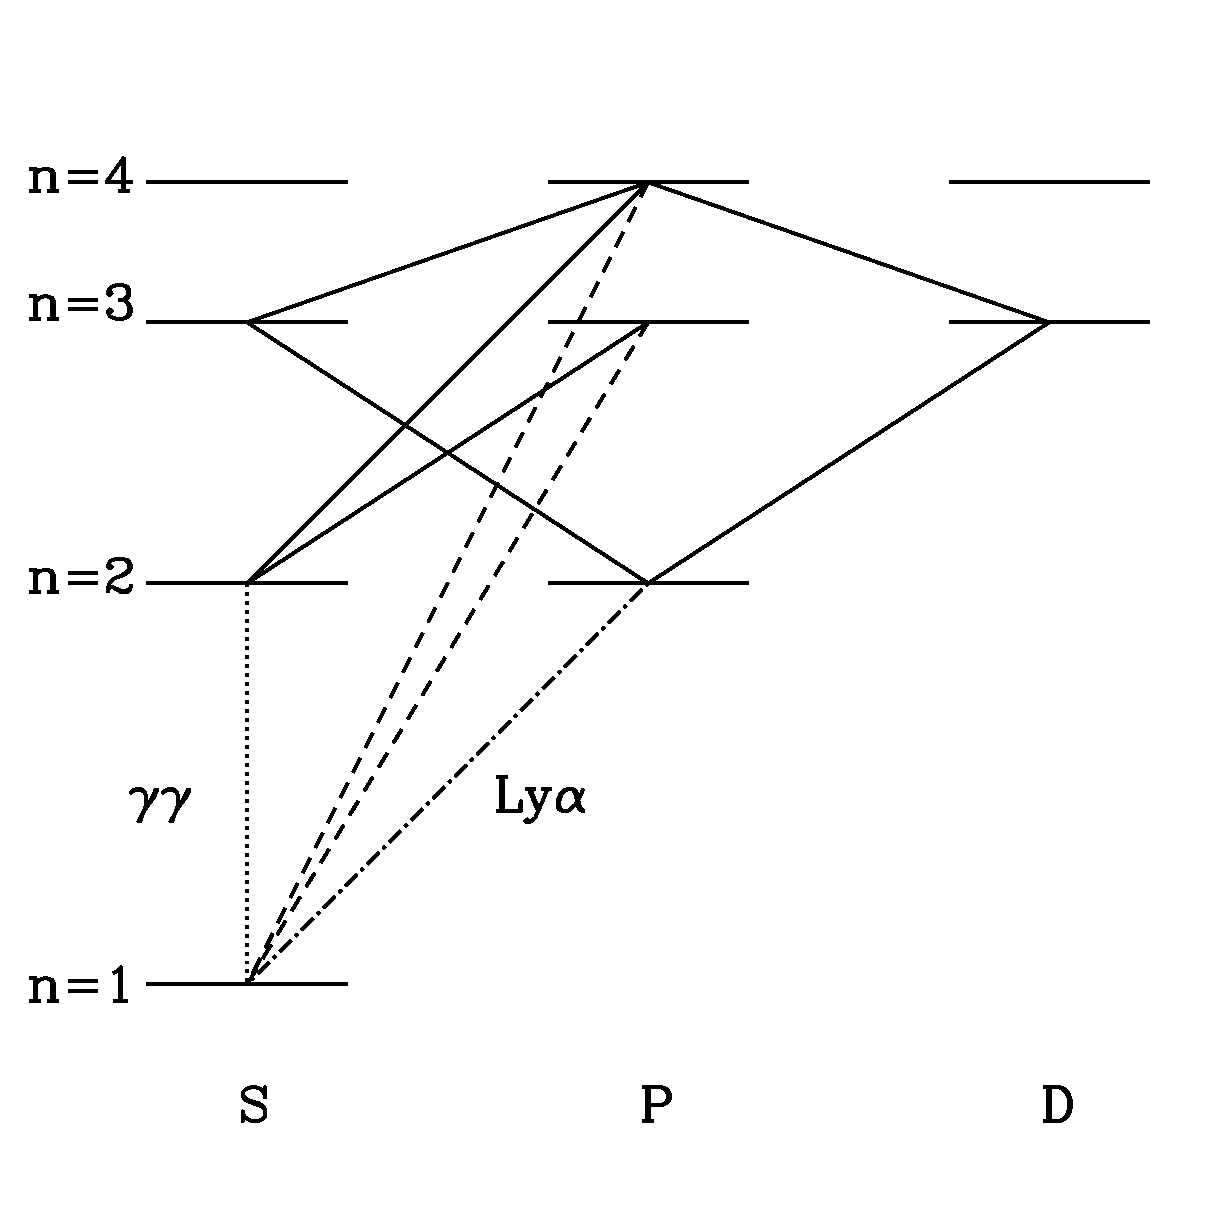
\includegraphics[width=0.6\textwidth]{Furlanetto/figure2-3}
\end{center}
\caption{Decay chains for Lyman-$\beta$ and Lyman-$\gamma$ excitations.  We show
  Lyman-$n$ transitions by dashed curves, Lyman-$\alpha$ by the dot-dashed
  curve, cascades by solid curves, and the forbidden $2S \rightarrow
  1S$ transition by the dotted curve. From \cite{pritchard06}.}
\label{fig:lygamma}
\end{figure}

The physics of the Wouthuysen-Field effect are actually much more complicated than naively expected because scattering itself modifies the shape of $J_\nu$ near the Lyman-$\alpha$ resonance \cite{chen04}. In essence, the spectrum must develop an absorption feature because of the increased scattering rate near the Lyman-$\alpha$ resonance. Photons lose energy at a fixed rate by redshifting, but each time they scatter they also lose a small amount of energy through recoil.  Momentum conservation during each scattering slightly decreases the frequency of the photon.  The strongly enhanced scattering rate near line center means that photons ``flow" through
that region more rapidly than elsewhere (where only the cosmological redshift applies), so the amplitude of the spectrum must be smaller.  Meanwhile, the scattering in such an optically thick medium also causes photons to diffuse away from line center, broadening the feature well beyond the nominal line width.

If the fractional frequency drift rate is denoted by ${\mathcal A}$, continuity requires $n_\nu {\mathcal A}=$~constant. Because ${\mathcal A}$ increases near resonance, the number density must fall.  On average, the energy loss (or gain) per scattering is \cite{chen04}
\begin{equation}
\frac{\Delta E_{\rm recoil}}{E} = \frac{h \nu}{m_p c^2} \, \left(1 - \frac{T_K}{T_c} \right),
\label{eq:recoil-loss}
\end{equation}
where the first factor comes from recoil off an isolated atom and the second factor corrects for the distribution of initial photon energies; the energy loss vanishes when $T_c = T_K$, and when $T_c < T_K$, the gas is heated by the scattering process.

To compute $S_\alpha$, we must calculate the photon spectrum near Lyman-$\alpha$.  We begin with the radiative
transfer equation in an expanding universe (written in comoving coordinates, and again using units of ~photons cm$^{-2}$ sr$^{-1}$ Hz$^{-1}$ s$^{-1}$ for $J_\nu$:
\begin{equation}
\frac{1}{c n_H \sigma_0} \, \frac{\partial J_\nu}{\partial t} = -\phi_\alpha(\nu) \, J_\nu + H \nu_\alpha \, \frac{\partial J_\nu}{\partial \nu} + \int d \nu' \, R(\nu,\nu') \, J_{\nu'} + C(t) \psi(\nu).
\label{eq:rt21}
\end{equation}
The first term on the right-hand side describes absorption, the second describes redshifting due to the Hubble flow, and the third accounts for re-emission following absorption.  $R(\nu,\nu')$ is the ``redistribution function" that specifies the frequency of an emitted photon, which depends on the relative momenta of the absorbed and
emitted photons as well as the absorbing atom. The last term accounts for the injection of new photons (via, e.g., radiative cascades that result in Lyman-$\alpha$ photons): $C$ is the rate at which they are produced and $\psi(\nu)$ is their frequency distribution.

The redistribution function $R$ is the difficult aspect of the problem, but it can be simplified if the frequency change per scattering (typically of order the absorption line width) is ``small."  In that case, we can expand $J_{\nu'}$ to second order in $(\nu-\nu')$ and rewrite equation~(\ref{eq:rt21}) as a diffusion problem in frequency.
The steady-state version of equation (\ref{eq:rt21}) becomes, in this so-called {\it Fokker-Planck} approximation, \cite{chen04}
\begin{equation}
\frac{d}{d x} \left( - {\mathcal A} \, J + {\mathcal D} \, \frac{d J}{d x} \right) + C \psi(x) = 0,
\label{eq:fokker}
\end{equation}
where $x \equiv (\nu-\nu_\alpha)/\Delta \nu_D$, $\Delta \nu_D$ is the Doppler width of the absorption profile, ${\mathcal A}$ is the frequency drift rate, and ${\mathcal D}$ is the diffusivity.  The Fokker-Planck approximation is valid so long as (i) the frequency change per scattering ($\sim \Delta \nu_D$) is smaller than the width of any spectral features, and either (iia) the photons are outside the line core where the Lyman-$\alpha$ line profile is slowly changing, or (iib) the atoms are in equilibrium with $T_c \approx T_K$.

Solving for the spectrum including scattering thus reduces to specifying ${\mathcal A}$ and ${\mathcal D}$.  The drift involves the Hubble flow, which sets ${\mathcal A}_H= - \tau_\alpha^{-1}$, where $\tau_\alpha$ is the Gunn-Peterson optical depth for the Lyman-$\alpha$ line \cite{gunn65, scheuer65}:
\begin{equation}
\tau_{\alpha} = \frac{\chi_\alpha \, n_{\rm HI}(z) \, c}{H(z) \nu_\alpha} \approx 3 \times 10^5 \, x_{\rm HI} \, \left( \frac{1+z}{7} \right)^{3/2}.
\label{eq:taugp}
\end{equation}
Because it is uniform, the Hubble flow does not introduce any diffusion. The remaining terms come from $R$ and
incorporate all the physical processes relevant to energy exchange in scattering.  The drift from recoil causes \cite{hirata06}
\begin{eqnarray}
{\mathcal D}_{\rm scatt} & = & \phi_\alpha(x)/2,
\label{eq:Dkin} \\
{\mathcal A}_{\rm scatt} & = &  -(\eta - x_0^{-1} ) \phi_\alpha(x),
\label{eq:Akin}
\end{eqnarray}
where $x_0 \equiv \nu_\alpha/\Delta \nu_D$ and $\eta \equiv (h \nu_\alpha^2)/(m_p c^2 \Delta \nu_D)$.  The latter is the recoil parameter measuring the average loss per scattering in units of the Doppler width.  The small energy defect between the hyperfine levels provides another source of slow energy exchange \cite{hirata06} and can be incorporated into the scattering in nearly the same way as recoil.

We can now solve equation~(\ref{eq:fokker}) once we choose the boundary conditions, which essentially correspond to the input photon spectrum (ignoring scattering) and the source function.  Because the
frequency range of interest is so narrow, two cases suffice: a flat input spectrum (which approximately describes photons that redshift through the Lyman-$\alpha$ resonance, regardless of the initial source spectrum)
and a step function, where photons are ``injected" at line center (through cascades or recombinations) and redshift away.  In either case, the first integral over $x$ in equation~(\ref{eq:fokker}) is trivial. At high temperatures where spin flips are unimportant to the overall energy exchange, we can write
\begin{equation}
\phi \frac{d J}{d x} + 2 \{ [\eta - (x + x_0)^{-1}] \phi + \tau_\alpha^{-1} \} J = 2 K / \tau_\alpha.
\label{eq:fokk-simp}
\end{equation}
The integration constant $K$ equals $J_\infty$, the flux far from resonance, both for photons that redshift into the line and for injected photons at $x<0$ (i.e., redward of line center); it is zero for injected photons at $x>0$.  

The formal analytic solution, when $K \neq 0$, is most compactly written in terms of $\delta_J \equiv (J_\infty -
J)/J_\infty$ \cite{chen04}:\footnote{Here we assume the gas has a sufficiently high temperature that the different hyperfine sub-transitions can be treated as one \cite{hirata06}.}
\begin{equation}
\delta_J(x) = 2 \eta \int_0^\infty d y \exp \left[ - 2 \{ \eta - (x+x_0)^{-1}\} y - {2 \over \tau_\alpha} \int_{x-y}^{x} \frac{d x'}{\phi_\alpha(x')} \right].
\label{eq:dj-soln}
\end{equation}
(An analogous form also exists for photons injected at line center.) The full problem, including the intrinsic Voigt profile of the Lyman-$\alpha$ line, must be solved numerically, but including only the Lorentzian wings from natural broadening allows a simpler solution \cite{furl06-lyheat}.  Fortunately, this assumption is quite accurate in the most interesting regime of  $T_K <  1000$~K.

%%%%%: FIGURE: Lyman-alpha spectral shape
\begin{figure}[]
\begin{center}
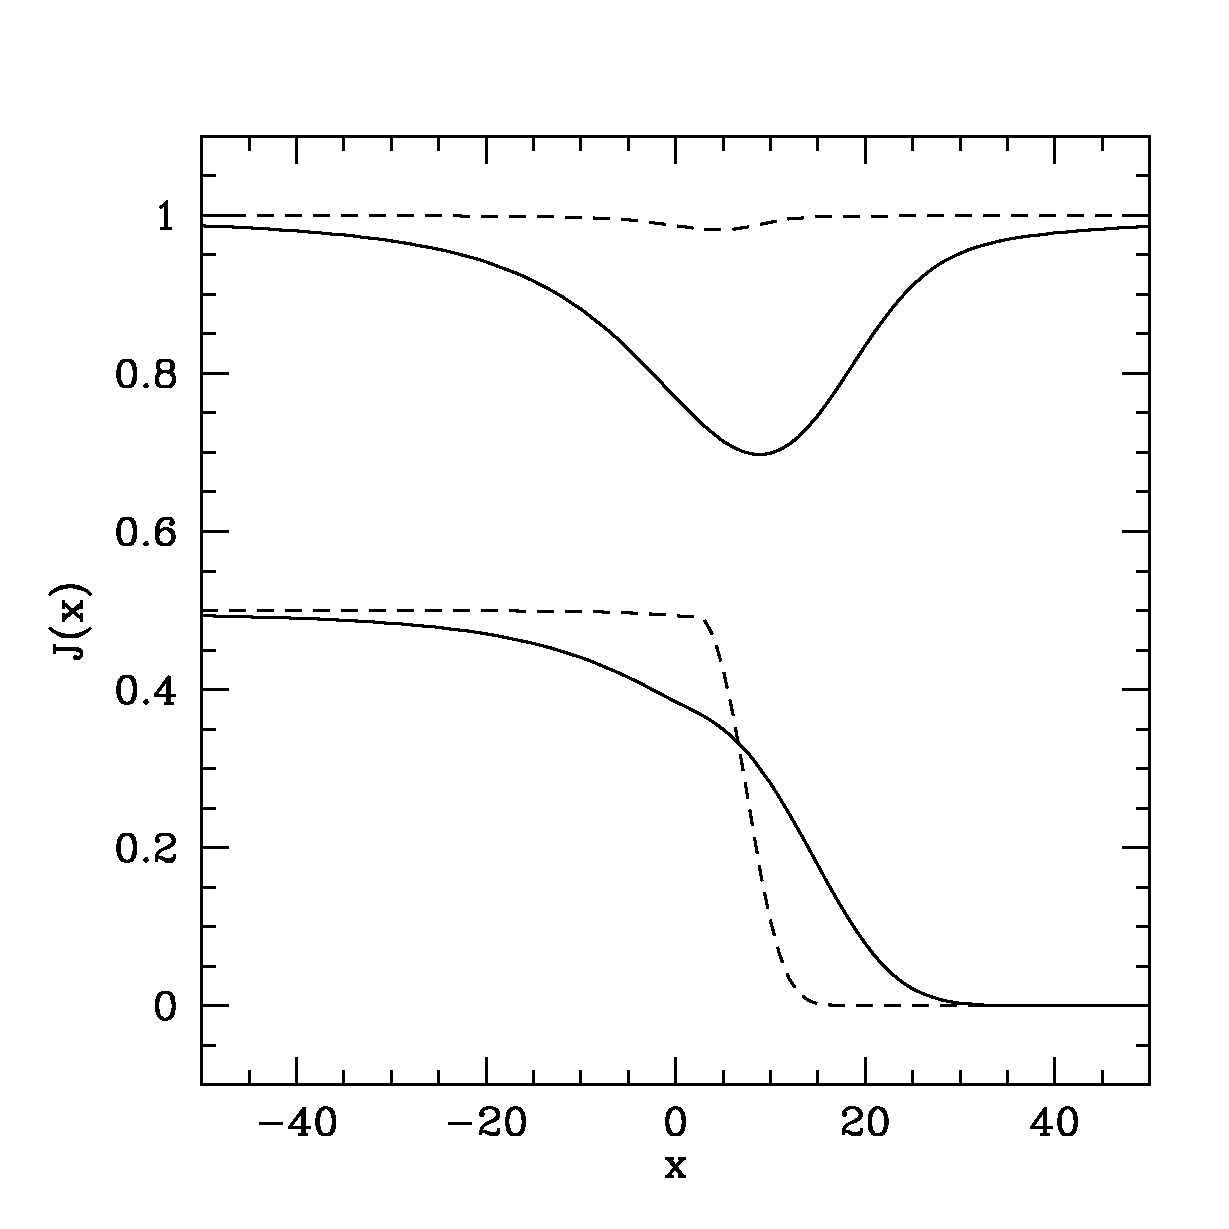
\includegraphics[width=0.6\textwidth]{Furlanetto/figure2-4}
\end{center}
\caption{Background radiation field near the Lyman-$\alpha$ resonance at $z=10$;
$x \equiv (\nu-\nu_\alpha)/\Delta \nu_D$ is the normalized deviation
from line center, in units of the Doppler width.  The upper and lower sets are for continuous photons
and photons injected at line center, respectively.  (The former are
normalized to $J_\infty$; the latter have arbitrary normalization.)
The solid and dashed curves take $T_K=10$ and $1000$~K,
respectively.  From \cite{furl06-lyheat}.}
\label{fig:lyshape}
\end{figure}

The crucial aspect of equation~(\ref{eq:dj-soln}) is that (as expected from the qualitative argument) an absorption feature appears near the line center, with its depth roughly proportional to $\eta$, our recoil parameter.  The feature is more significant when $T_K$ is small (because in that case the average effect of recoil is large). Figure~\ref{fig:lyshape} shows some example spectra (both for a continuous background and for photons injected at line center).

Usually, the most important consequence is the suppression of the radiation spectrum at line center compared to the assumed initial condition.  This decreases the total scattering rate of Lyman-$\alpha$ photons (and hence the Wouthuysen-Field coupling), with the suppression factor (defined in equation~\ref{eq:xalpha}) as \cite{chen04} 
\begin{equation}
S_\alpha = \int_{-\infty}^\infty d x \, \phi_\alpha(x)\, J(x) \approx
[1 - \delta_J(0)] \le 1,
\label{eq:salpha-defn}
\end{equation}
where the second equality follows from the narrowness of the line profile.  Again, the Lorentzian wing approximation turns out to be an excellent one; when $T_K \gg T_\star$, the suppression is \cite{furl06-lyheat}
\begin{equation} S_\alpha \sim \exp \left[ -0.803 \left({T_K\over
1~{\rm K}}\right)^{-2/3} \left( \frac{\tau_\alpha}{10^{6}}
\right)^{1/3} \right].
\label{eq:salpha-approx}
\end{equation}
Note that this form applies to both photons injected at line center as well as those that redshift in from infinity.  As we can see in Figure~\ref{fig:lyshape}, the suppression is most significant in cool gas.


\section{Heating of the Intergalactic Medium} 

We have seen that both collisions and the Wouthuysen-Field effect couple the spin temperature to the kinetic temperature of the gas. The 21-cm brightness temperature therefore depends on processes that heat the IGM. We will review several such mechanisms in this section.

\subsection{The Lyman-$\alpha$ Background}

The photons that trigger Lyman-$\alpha$ coupling exchange energy with the IGM, through the recoil in each scattering event. The typical energy exchange per scattering is small (see eq. \ref{eq:recoil-loss}), but the scattering rate is extremely large.  If the net heating rate per atom followed the naive expectation, $\sim
P_\alpha \times (h \nu_\alpha)^2/m_p c^2$, the kinetic temperature would surpass $T_\gamma$ soon after Wouthuysen-Field coupling becomes efficient.

However, the details of radiative transfer radically change these expectations \cite{chen04}.  In a static medium, the energy exchange \emph{must} vanish in equilibrium even though scattering continues at nearly the same rate.
Scattering induces an asymmetric absorption feature near $\nu_\alpha$ (Figure~\ref{fig:lyshape}) whose shape depends on the combined effects of atomic recoils and the scattering diffusivity.  In equilibrium, the latter exactly counterbalances the former.  

If we removed scattering, the absorption feature would redshift away as the Universe expands. Thus, the energy exchange rate from scattering must simply be that required to maintain the feature in place.  For photons redshifting into resonance, the absorption trough has total energy 
\begin{equation}
\Delta u_\alpha = (4\pi/c) \int (J_\infty - J_\nu) h \nu d \nu,
\end{equation}
where $J_\infty$ is the input spectrum, and we note that the $h \nu$ factor converts from our definition of specific intensity (which counts photons) to energy.  The radiation background loses $\epsilon_\alpha = H \Delta u_\alpha$ per
unit time through redshifting; this energy goes into heating the gas.
Relative to adiabatic cooling by the Hubble expansion, the fractional
heating amplitude is
\begin{eqnarray}
\frac{2}{3} \, \frac{\epsilon_\alpha}{k_B T_K n_H H(z) } & = & \frac{8 \pi}{3} \, \frac{h \nu_\alpha}{k_B T_K} \, \frac{J_\infty \, \Delta \nu_D}{c n_H} \, \int_{-\infty}^{\infty} d x \delta_J(x) \label{eq:epsalpha}
\\
& \approx & \frac{0.80}{T_K^{4/3}} \, \frac{x_\alpha}{S_\alpha} \left( \frac{10}{1+z} \right),
\label{eq:lyaheat}
\end{eqnarray}
Here we have evaluated the integral for the continuum photons that
redshift into the Lyman-$\alpha$ resonance; the ``injected" photons
actually cool the gas slightly.  The net energy exchange when
Wouthuysen-Field coupling becomes important (at $x_\alpha \sim
S_\alpha$) is therefore just a fraction of a degree, and in practice gas heating through Lyman-$\alpha$ scattering
is generally unimportant \cite{chen04,furl06-lyheat}.

Fundamentally, Lyman-$\alpha$ heating is inefficient because scattering diffusivity cancels the effects of recoil.  From Figure~\ref{fig:lyshape}, we see that the background spectrum is weaker on the blue side of the line than on the red.  The scattering process tends to move the photon toward line center, with the extra energy deposited in or extracted from the gas.  Because more scattering occurs on the red side, this tends to transfer energy from the gas back to the photons, mostly canceling the energy obtained through recoil.

\subsection{The Cosmic Microwave Background} 

The previous section shows that, when considered as a two-level process that acts in isolation, Lyman-$\alpha$ scattering has only a slight effect on the gas temperature. However, in reality this Lyman-$\alpha$ scattering always occurs in conjunction with scattering of CMB photons within the 21-cm transition. The combination leads to an enhanced heating rate \cite{venumadhav18}.

In essence, the process works as follows. The CMB photons scatter through the hyperfine levels of HI to heat those atoms above their expected temperature (determined in this simple case by adiabatic cooling). Meanwhile, Lyman-$\alpha$ photons scatter through the gas as well. As they do so, they mix the hyperfine levels of the HI ground state, as depicted in Figure~\ref{fig:wf} -- this is the Wouthuysen-Field effect. CMB scattering continues to heat the hyperfine level populations during the Lyman-$\alpha$ scattering, which then sweeps up this extra energy and ultimately deposits it as thermal energy through the net recoil effect.

We can estimate the energy available to this heating mechanism by considering the CMB energy reservoir \cite{venumadhav18}. The CMB energy density at the 21-cm transition is $u_\nu = (4 \pi/c) B_\nu \approx 8 \pi (\nu_{21}^2/c^3) k_B T_\gamma$. Over a redshift interval $\Delta z=1$, the total energy that redshifts through the line is $u_\nu \Delta \nu \approx 8 \pi (\nu_{21}/c)^3 k_B T_\gamma / (1+z)^2$. However, only a fraction $\tau_{10}$ actually interacts with the line. If all of this energy is used for heating, the temperature change per H atom would be
\begin{equation}
\Delta T_{\rm CMB-Ly\alpha} \approx \tau_{10} {u_\nu \Delta_\nu \over (3/2) n_H} \approx 5 x_{\rm HI} \  \left( {1 + z \over 20} \right)^{-1/2} \left( {10 \ {\rm K} \over T_S} \right) \ {\rm K}.
\label{eq:cmb-lya-heat}
\end{equation}

A more detailed calculation of the heating rate shows that it is somewhat slower, but it does amplify the effect of the Lyman-$\alpha$ heating alone by a factor of several \cite{venumadhav18}. In standard models of the early radiation backgrounds, the correction is still relatively modest, but it is not negligible. For example, in the fiducial model considered by \cite{venumadhav18}, the Lyman-$\alpha$ heating on its own modifies $T_K$ by $\sim 1$--5\%, but with the CMB scattering included the effect is $\sim 9$--15\%. Additionally, the CMB scattering can be enhanced in some exotic physics models that decrease the spin temperature substantially.

\subsection{The X-ray Background} 

Because they have relatively long mean free paths, X-rays from galaxies and quasars are likely to be the most important heating agent for the low-density IGM  \cite{madau97}.  In particular, photons with $E>1.5 x_{\rm HI}^{1/3} [(1+z)/10]^{1/2}$~keV have mean free paths exceeding the Hubble length \cite{oh01}.  Lower-energy X-rays will be absorbed in the IGM, depositing much of their energy as heat, as will a fraction of higher-energy X-rays.

X-rays heat the IGM gas by first photoionizing a hydrogen or helium atom.  The resulting ``primary'' electron retains most of the photon energy (aside from that required to ionize it) as kinetic energy, which it must then distribute to the general IGM through three main channels: (1) collisional ionizations, which produce more secondary electrons that themselves scatter through the IGM, (2) collisional excitations of HeI (which produce photons capable of ionizing HI) and HI (which produces a Lyman-$\alpha$ background), and (3) Coulomb collisions with free electrons (which distributes the kinetic energy .  The relative cross-sections of these processes determines what fraction of the X-ray energy goes to heating ($f_{\rm heat}$), ionization ($f_{\rm ion}$), and excitation ($f_{\rm excite}$); clearly it depends on both the ionized fraction $x_i$ and the input photon energy.  Through these scatterings, the primary photoelectrons, with $T \sim 10^6$~K, rapidly cool to energies just below the Lyman-$\alpha$ threshold, $<10$~eV, and thus equilibrate with the other IGM electrons.  After that, the electrons and neutrals equilibrate through elastic scattering on a timescale $t_{\rm eq} \sim 5 [10/(1+z)]^3$~Myr.  Because $t_{\rm eq} \ll H(z)^{-1}$, the assumption of a single temperature fluid is an excellent one.

%%%%%: FIGURE: X-ray heating
\begin{figure}[]
\begin{center}
\includegraphics[width=0.4\textwidth]{Furlanetto/figure2-5a} 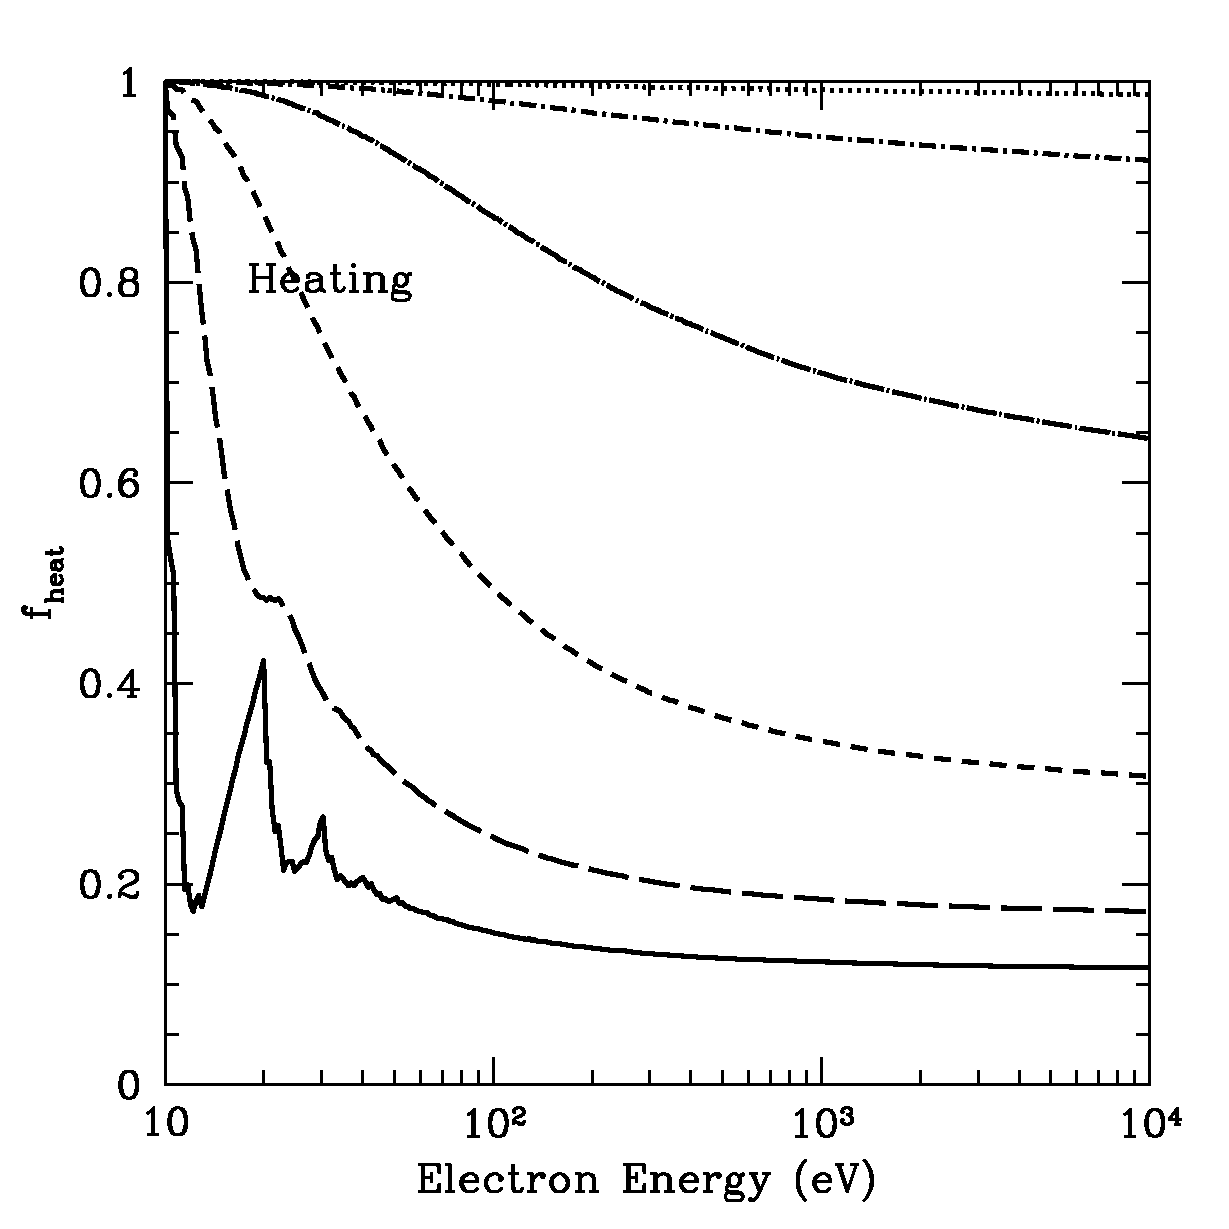
\includegraphics[width=0.4\textwidth]{Furlanetto/figure2-5b} \\
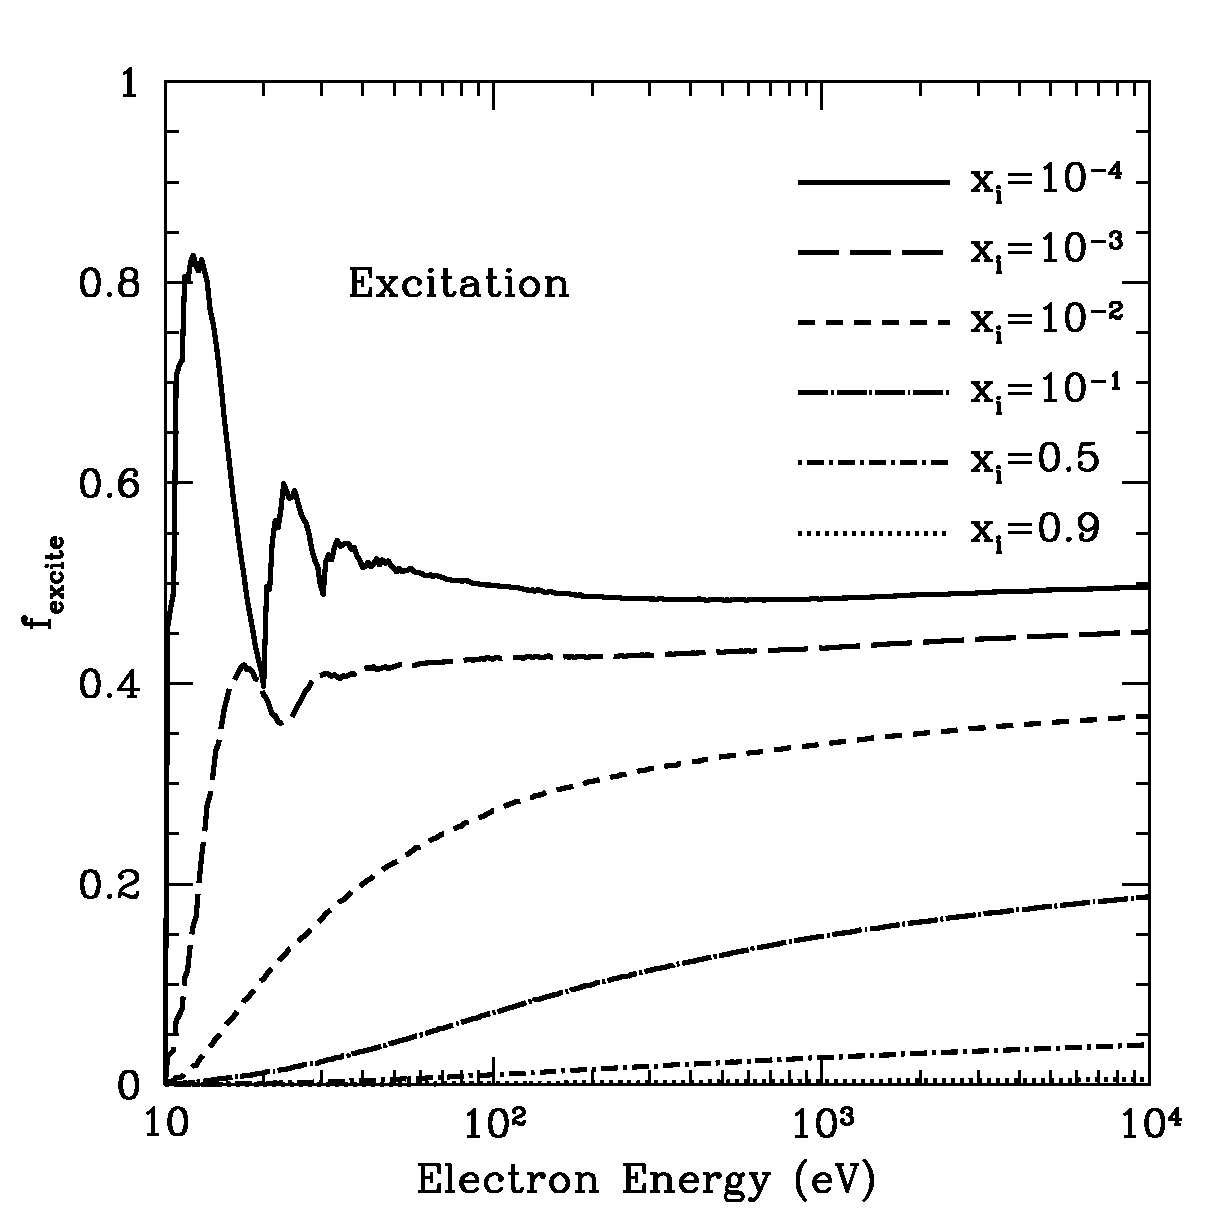
\includegraphics[width=0.4\textwidth]{Furlanetto/figure2-5c} 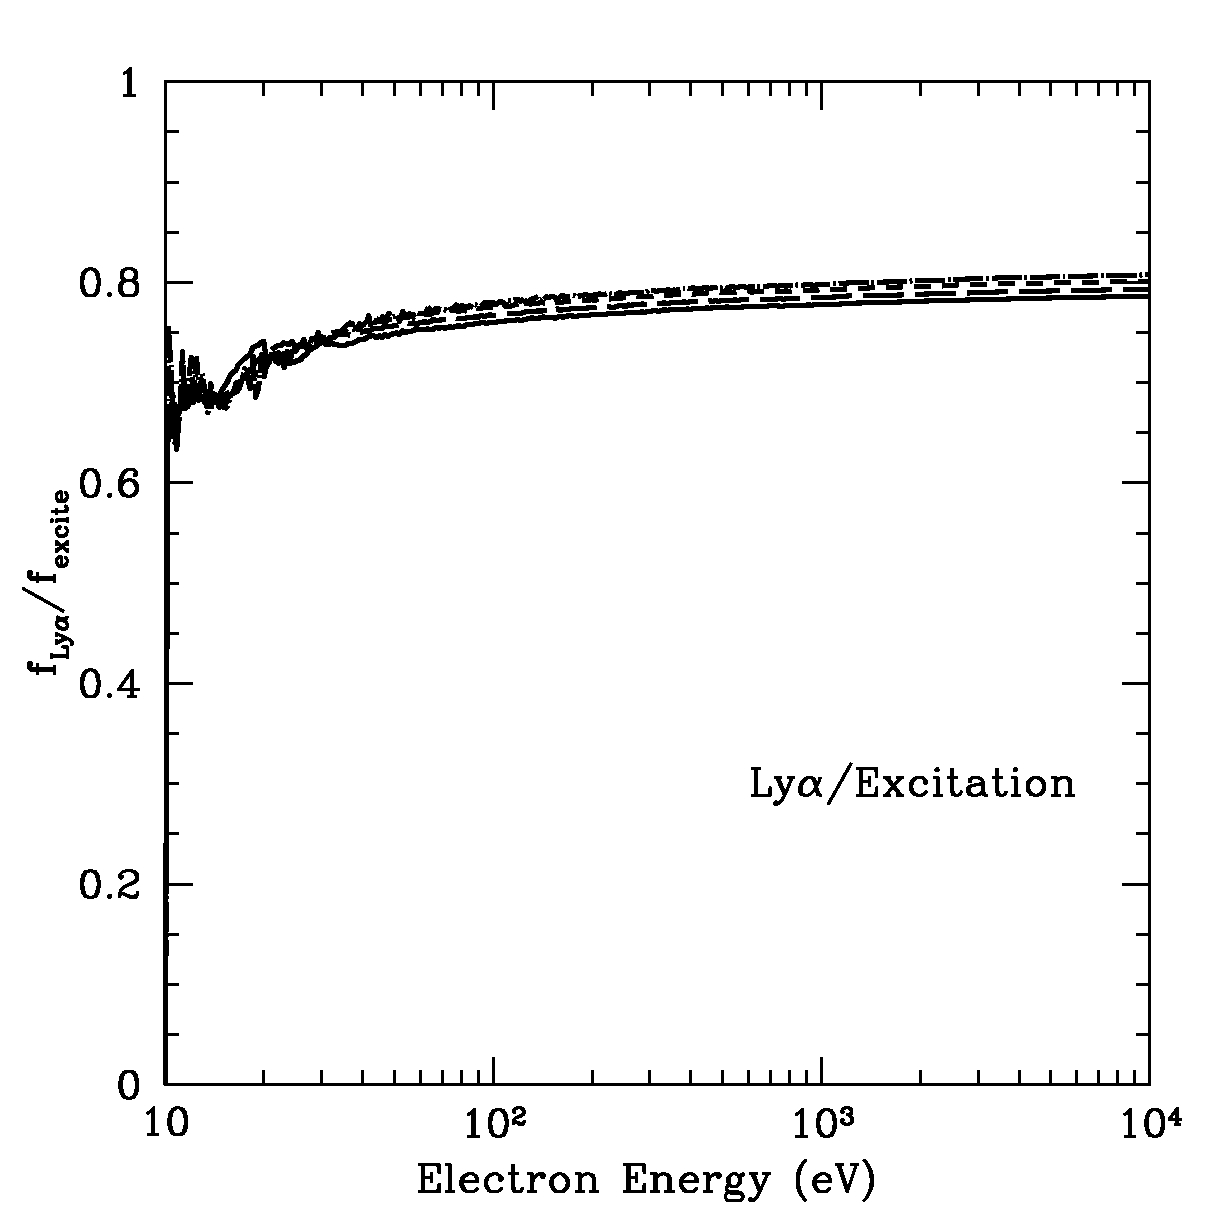
\includegraphics[width=0.4\textwidth]{Furlanetto/figure2-5d}
\end{center}
\caption{Energy deposition from fast electrons. We show the fraction of the initial energy deposited in ionization (upper left), heating (upper right), and collisional excitation (lower left), as a function of electron energy and for several different ionized fractions $x_i$. The lower right shows the fraction of the collisional excitation energy deposited in the HI Lyman-$\alpha$ transition, $f_{\rm Ly\alpha}$.  From \cite{furl10-xray}.}
\label{fig:xrayheat}
\end{figure}

The details of this process have been examined numerically \cite{shull85,valdes08,furl10-xray}, and Figure~\ref{fig:xrayheat} shows some example results. Note that the deposition fractions are smooth functions at high electron energies but, at low energies -- where the atomic energy levels become relevant -- can be quite complex. A number of approximate fits have been presented for the high-energy regime \cite{ricotti02, volonteri09}, but they are not accurate over the full energy range. A crude but useful approximation to the high-energy limit often suffices \cite{chen04-decay}:
\begin{eqnarray}
f_{\rm heat} & \sim & (1+2 x_i)/3 \nonumber \\
f_{\rm ion} \sim f_{\rm excite} & \sim & (1-x_i)/3,
\label{eq:fxapprox}
\end{eqnarray}
where $x_i$ is the ionized fraction. In highly ionized gas, collisions with free electrons dominate and $f_{\rm heat} \rightarrow 1$; in the opposite limit, the energy is split roughly equally between these three processes. However, the complexity of the behavior at low electron energies -- together with the increasing optical thickness of the IGM in that regime, and the fact that most sources are brighter in this soft X-ray regime -- suggest that a more careful treatment is needed for accurate work. \cite{furl10-xray} recommend interpolating the exact results.

\bibliographystyle{plain}
\bibliography{Furlanetto/ch2-refs}


\newcommand*{\dt}[1]{%
  \accentset{\mbox{\large\bfseries .}}{#1}}
\newcommand*{\ddt}[1]{%
  \accentset{\mbox{\large\bfseries .\hspace{-0.25ex}.}}{#1}}

% Journals
\newcommand{\aj}{{\it AJ}}
\newcommand{\apj}{{\it ApJ}}
\newcommand{\mnras}{{\it MNRAS}}
\newcommand{\aap}{{\it A\&A}}
\newcommand{\pasj}{{\it PASJ}}
\newcommand{\pasa}{{\it PASA}}
\newcommand{\pr}{{\it PR}}
\newcommand{\asr}{{\it ASR}}
\newcommand{\nat}{{\it Nat}}

% Densities
\newcommand{\nH}{n_{\text{H}}}
\newcommand{\nHe}{n_{\text{He}}}
\newcommand{\nHbar}{\bar{n}_{\text{H}}^0}
\newcommand{\nHebar}{\bar{n}_{\text{He}}^0}
\newcommand{\nbbar}{\bar{n}_{\text{b}}^0}
\newcommand{\rhobbar}{\bar{rho}_{\text{b}}^0}

% Hydrogen and helium ions - don't add $$
\newcommand{\HI}{\text{H} {\textsc{i}}}
\newcommand{\HII}{\text{H} {\textsc{ii}}}
\newcommand{\HeI}{\text{He} {\textsc{i}}}
\newcommand{\HeII}{\text{He} {\textsc{ii}}}
\newcommand{\HeIII}{\text{He} {\textsc{iii}}}
\newcommand{\Htwo}{\text{H}_2}
\newcommand{\Hatom}{\text{H}}
\newcommand{\xibar}{\overline{x}_i}
\newcommand{\QHII}{Q_{\HII}}

\newcommand{\xipr}{x_i^{\prime}}

% Number densities of common ions
\newcommand{\nHI}{n_{\text{H } \textsc{i}}}
\newcommand{\nHII}{n_{\text{H } \textsc{ii}}}
\newcommand{\nHeI}{n_{\text{He } \textsc{i}}}
\newcommand{\nHeII}{n_{\text{He } \textsc{ii}}}
\newcommand{\nHeIII}{n_{\text{He } \textsc{iii}}}
\newcommand{\nel}{n_{\text{e}}}  
\newcommand{\ntot}{n_{\text{tot}}}

% Species fractions
\newcommand{\xHI}{x_{\text{H } \textsc{i}}}
\newcommand{\xHII}{x_{\text{H } \textsc{ii}}}
\newcommand{\xHeI}{x_{\text{He } \textsc{i}}}
\newcommand{\xHeII}{x_{\text{He } \textsc{ii}}}
\newcommand{\xHeIII}{x_{\text{He } \textsc{iii}}}

% Ionization & Recombination coefficients
\newcommand{\ionHI}{\Gamma_{\text{H } \textsc{i}}}
\newcommand{\ionHeI}{\Gamma_{\text{He } \textsc{i}}}
\newcommand{\ionHeII}{\Gamma_{\text{He } \textsc{ii}}}
\newcommand{\ionsecHI}{\gamma_{\text{H } \textsc{i}}}
\newcommand{\ionsecHeI}{\gamma_{\text{He } \textsc{i}}}
\newcommand{\ionsecHeII}{\gamma_{\text{He } \textsc{ii}}}
\newcommand{\ioncollHI}{\beta_{\text{H } \textsc{i}}}
\newcommand{\ioncollHeI}{\beta_{\text{He } \textsc{i}}}
\newcommand{\ioncollHeII}{\beta_{\text{He } \textsc{ii}}}
\newcommand{\recHII}{\alpha_{\text{H } \textsc{ii}}}
\newcommand{\recHeII}{\alpha_{\text{He } \textsc{ii}}}
\newcommand{\recHeIII}{\alpha_{\text{He } \textsc{iii}}}

\newcommand{\xiHeII}{\xi_{\text{He} \textsc{ii}}}

% Heating rate coefficients
\newcommand{\heatHI}{\mathcal{H}_{\text{H } \textsc{i}}}
\newcommand{\heatHeI}{\mathcal{H}_{\text{He } \textsc{i}}}
\newcommand{\heatHeII}{\mathcal{H}_{\text{He } \textsc{ii}}}

% Cooling rate coefficients
\newcommand{\cooldielHeII}{\omega_{\text{He } \textsc{ii}}}

% Phi and Psi
\newcommand{\PhiHI}{\Phi_{\text{H } \textsc{i}}}
\newcommand{\PhiHeI}{\Phi_{\text{He } \textsc{i}}}
\newcommand{\PhiHeII}{\Phi_{\text{He } \textsc{ii}}}
\newcommand{\PsiHI}{\Psi_{\text{H } \textsc{i}}}
\newcommand{\PsiHeI}{\Psi_{\text{He } \textsc{i}}}
\newcommand{\PsiHeII}{\Psi_{\text{He } \textsc{ii}}}

% BH stuff
\newcommand{\fduty}{f_{\text{duty}}}
\newcommand{\Cedd}{C_{\text{edd}}}
\newcommand{\tedd}{t_{\text{edd}}}
\newcommand{\Mbh}{M_{\bullet}}

\newcommand{\SFR}{\dot{M}_{\ast}}
\newcommand{\MAR}{\dot{M}_{b}}
\newcommand{\SFE}{f_{\ast}}
\newcommand{\Tmin}{T_{\min}}

% Random
\newcommand{\zprime}{z^{\prime}}
\newcommand{\dprime}{\prime\prime}
\newcommand{\fstar}{f_{\ast}}
\newcommand{\fstarbh}{\tilde{\fstar}}
\newcommand{\fbh}{f_{\bullet}}
\newcommand{\fcoll}{f_{\text{coll}}}
\newcommand{\dfcolldz}{\frac{df_{\text{coll}}}{dz}}
\newcommand{\dfcolldt}{\frac{df_{\text{coll}}}{dt}}
\newcommand{\dfcolldzbh}{\frac{d\tilde{f}_{\text{coll}}}{dz}}
\newcommand{\dfcolldtbh}{\frac{d\tilde{f}_{\text{coll}}}{dt}}
\newcommand{\mmin}{m_{\text{min}}}
\newcommand{\rhobh}{\rho_{\bullet}}
\newcommand{\rhobhdot}{\dt{\rho}_{\bullet}}
\newcommand{\rhostar}{\rho_{\ast}}
\newcommand{\rhostardot}{\dt{\rho}_{\ast}}
\newcommand{\rhostarbhdot}{\dt{\rho}_{\ast\bullet}}
\newcommand{\rhom}{\rho_m}
\newcommand{\fstardegen}{f_{\ast \bullet}}
\newcommand{\Nion}{N_{\text{ion}}}
\newcommand{\Ndot}{\dot{N}_{\text{ion}}}
\newcommand{\fesc}{f_{\text{esc}}}
\newcommand{\nmax}{n_{\text{max}}}
\newcommand{\frec}{f_{\text{rec}}}
\newcommand{\frecn}{f_{\text{rec}}^{n}}
\newcommand{\frecbar}{\overline{f}_{\text{rec}}}
\newcommand{\Msun}{M_{\odot}}

\newcommand{\SFRunits}{M_{\odot} \ \text{s}^{-1}}
\newcommand{\fbin}{f_{\text{bin}}}
\newcommand{\fact}{f_{\text{act}}}
\newcommand{\fsurv}{f_{\text{surv}}}

\newcommand{\JLW}{J_{\text{LW}}}

\newcommand{\fion}{f_{\text{ion}}}
\newcommand{\nnu}{$n_{\nu}$}
\newcommand{\ncol}{N_i}
\newcommand{\Tvir}{T_{\text{vir}}}


\newcommand{\emissivity}{\text{erg} \ \text{s}^{-1} \ \text{Hz}^{-1} \ \text{cMpc}^{-3}}

\newcommand{\Ja}{J_{\alpha}}
\newcommand{\Lya}{\text{Ly-}\alpha}
\newcommand{\Lyn}{\text{Ly-}n}
\newcommand{\TS}{T_{\text{S}}}
\newcommand{\TK}{T_{\text{K}}}
\newcommand{\Tcmb}{T_{\text{CMB}}}
\newcommand{\TCMB}{T_{\text{CMB}}}
\newcommand{\TR}{T_{\text{R}}}

% Physical constants
\newcommand{\kB}{k_{\text{B}}}



\newcommand{\fheat}{f^{\text{heat}}}
\newcommand{\fXh}{f_{X,h}}
\newcommand{\fioni}{f_i^{\text{ion}}}
\newcommand{\Lbol}{\mathcal{L}_{\text{bol}}}
\newcommand{\spec}{\mathcal{N}}
\newcommand{\Heat}{\mathcal{H}}
\newcommand{\trec}{$t_{\text{rec}}$}
\newcommand{\Lbox}{L_{\mathrm{box}}}
\newcommand{\dx}{\Delta x}
\newcommand{\dd}{\text{d}}

\newcommand{\drIF}{$\Delta r_{\mathrm{IF}}$}
\newcommand{\dTb}{$\delta T_b$}
\newcommand{\Nvec}{\mathbf{N}}
\newcommand{\sh}{\mathrm{sh}}
\newcommand{\Mdot}{\dot{M}}
\newcommand{\Ledd}{L_{\text{edd}}}

\newcommand{\intensityunitsnumber}{\text{s}^{-1} \ \text{cm}^{-2} \ \mathrm{Hz}^{-1} \ \text{sr}^{-1}}


\chapter{Astrophysics from the 21-cm background}

\begin{bf}
  \author{Jordan Mirocha}\\
\\
\end{bf}

The goal of this chapter is to describe the astrophysics encoded by the 21-cm background. We will begin in \S\ref{sec:RT} with a general introduction to radiative transfer and ionization chemistry in gas of primordial composition. Then, we will discuss techniques to model the key dependencies of the 21-cm background, i.e., the ionization and temperature fields \S\ref{sec:xi_Tk_Ja}. In \S\ref{sec:sources}, we will provide a review of the most plausible sources of ionization and heating in the early Universe, while in \S\ref{sec:predictions}, we will summarize the status of current predictions and highlight the modeling tools available today.


\section{Notes about Organization}

May 5:
\begin{itemize}
	\item Might make sense to combine sections 3 and 4 in my outline, i.e, introduce sources and current predictions for their properties all in one go.
	\item Have a table somewhere of common parameters for Brad to point to.
	\item In modeling section, group by codes or techniques? Separate section for galaxy SAMs?
	\item Start section 2 with general RT background, move into approximations later?
	\item What figures should I include? Start collecting them.
\end{itemize}

Figures 
\begin{itemize}
	\item Picture of reionization simulation.
	\item Schematic of ray tracing
	\item Show 1-D profiles to build intuition?
	\item Stellar spectra
	\item XRB spectra 
	\item Empirical constraints on $L_X$-SFR.
	\item 
\end{itemize}


Here's my approach:
\begin{itemize}
	\item Talk about how 21-cm traces ionization and heating. Outline generic non-Eq chemistry setup and how one would do this in ``all its glory.''
	\item Motivate separation of ionization and heating (mean free path), and how that allows more approximate techniques. Outline those approximate techniques.
	\item Turn to the sources. We've discussed how to model ionization and heating but not what the source terms are. 
	\item Put it all together: basic predictions. Intuition for timing of different features in global signal and power spectrum, prospects for breaking degeneracies between different sources/parameters.
	\item Models. Discussion of available tools, differences, progress? Lump in with previous section.
\end{itemize}


%%%
%% Ionization, thermal, and Ly-a histories
%%%
\section{Components of the 21-cm Background} \label{sec:RT}

% T_21
\subsection{The brightness temperature}
The differential brightness temperature of a patch of the IGM at redshift $z$ and position $\mathbf{x}$ is given by\footnote{Check out Chapter 1 for a detailed derivation.} 
\begin{equation}
    \delta T_b(z, \mathbf{x}) \simeq 27 (1 + \boldmath{\delta}) (1 - \mathbf{x_i}) \left(\frac{\Omega_{b,0} h^2}{0.023} \right) \left(\frac{0.15}{\Omega_{m,0} h^2} \frac{1 + z}{10} \right)^{1/2} \left(1 - \frac{T_R}{\mathbf{T_S}} \right) , \label{eq:dTb}
\end{equation}
where $\mathbf{\delta}$ is the baryonic overdensity relative to the cosmic mean, $x_i$ is the ionized fraction, $T_R$ is the radiation background temperature (generally the CMB, $T_R = T_{\gamma}$), and
\begin{equation}
    \mathbf{T_S}^{-1} \approx \frac{T_R^{-1} + \mathbf{x_c} \mathbf{T_K}^{-1} + \mathbf{x_{\alpha}} \mathbf{T_{\alpha}}^{-1}}{1 + x_c + x_{\alpha}} . \label{eq:Ts}
\end{equation}
is the spin temperature, which quantifies the level populations in the ground state of the hydrogen atom, and itself depends on the kinetic temperature, $T_K$, and ``colour temperature'' of the Lyman-$\alpha$ radiation background, $T_{\alpha}$. Because the IGM is optically thick to Ly-$\alpha$ photons, the approximation $T_K \approx T_{\alpha}$ is generally very accurate.

The collisional coupling coefficients\footnote{For a more detailed introduction to collisional and radiative coupling, see Chapter 1.}, $x_c$, themselves depend on the gas density, ionization state, and temperature, and can be computed as a function of temperature from tabulated values in \cite{Zygelman2005}. The radiative coupling coefficient, $x_{\alpha}$, depends on the Ly-$\alpha$ intensity, $J_{\alpha}$, via
\begin{equation}
    x_{\alpha} = \frac{S_{\alpha}}{1+z} \frac{\hat{J}_{\alpha}}{{J}_{\alpha,0}} \label{eq:Jalpha}
\end{equation}
where
\begin{equation}
    J_{\alpha,0} \equiv \frac{16\pi^2 T_{\star} e^2 f_{\alpha}}{27 A_{10} T_{\gamma,0} m_e c} . 
\end{equation}
$\hat{J}_{\alpha}$ is the angle-averaged intensity of Ly-$\alpha$ photons in
units of $\intensityunitsnumber$, $S_{\alpha}$ is a correction factor that
accounts for variations in the background intensity near line-center
\cite{Chen2004,FurlanettoPritchard2006,Hirata2006}, $m_e$ and $e$ are the
electron mass and charge, respectively, $f_{\alpha}$ is the $\Lya$ oscillator
strength, and $A_{10}$ is the Einstein A coefficient for the 21-cm transition.

This is all to point out that we care about the electron fraction, kinetic temperature, and Ly-$\alpha$ radiation field.

The key quantities moving forward are $x_i$, $T_K$, and $J_{\alpha}$. The tricky part about doing this modeling is that these state variables depend on the \textit{history} of ionization, heating, and Ly-$\alpha$ emission. 

Notes about notation:
\begin{itemize}
	\item We use boldface to indicate quantifies with a positional dependence. Is this going to be super tedious?
\end{itemize}

Questions moving forward:
\begin{itemize}
	\item Start on large scales, move down to small scales?
	\item When to make the distinction between local and global quantities?
\end{itemize}

Best approach for evolution: go in reverse time order, from reionization to Lya stuff, in each section do local and global.

% Global signal
\subsubsection{The ``global'' 21-cm signal}
On very large scales...
\begin{align}
    \delta T_b \simeq 27 (1 - \mathbf{x_i}) \left(\frac{\Omega_{b,0} h^2}{0.023} \right) \left(\frac{0.15}{\Omega_{m,0} h^2} \frac{1 + z}{10} \right)^{1/2} \left(1 - \frac{T_R}{T_S} \right) , \label{eq:dTb}
\end{align}

Many experiments are targeting this signal. For this reason, modeling efforts for the global signal often take an approximate approach. Under the assumption that fluctuations in $\delta$, $x_i$, and $T_S$ are uncorrelated, the volume-averaged differential brightness temperature is simply related to the volume-averaged density, ionization fraction, and spin temperature. Averaging over large volumes means $\delta \approx 0$, and while in general these fields \textit{will} be correlated, {\color{red} the effects are likely minor: cite that one paper that Xueli Chen is on.}


In the next three sections, we walk through the main epochs of evolution relevant to the 21-cm background, starting with reionization, and working our way backwards in time to first light. As in this section, boldfaced symbols refer to variables with an implicit spatial dependence, while regularly typset symbols refer to the spatial average. {\color{red} is this too tedious?}

Talk here about how in numerical simulations we would just do radiative transfer so there's no need to break up all these things. But, RT is expensive, so in practice most models (at least those used for inference) make approximations, and it is very convenient to consider

%%
% RT background?
%%
\subsection{Basics of Non-Equilibrium Ionization Chemistry}
As described in the previous section, the 21-cm brightness temperature of a patch of the IGM depends on the ionization and thermal state of the gas, as well as the incident Ly-$\alpha$ intensity\footnote{Note that Ly-$\alpha$ photons can transfer energy to the gas though we omit this dependence from the current discussion (see \S1).}. The evolution of the ionization and temperature are coupled, and so must be evolved self-consistently. The number density of hydrogen and helium ions in a static medium evolve as
\begin{align}
    \frac{d \nHII}{dt} & = (\ionHI + \ionsecHI + \ioncollHI \nel) \nHI - \recHII \nel \nHII   \label{eq:HIIRateEquation} \\
    \frac{d \nHeII}{dt} & = (\ionHeI + \ionsecHeI + \ioncollHeI \nel) \nHeI \nonumber + \recHeIII \nel \nHeIII  - (\ioncollHeII + \recHeII + \xiHeII) \nel \nHeII \\ & - (\ionHeII + \ionsecHeII) \nHeII \label{eq:HeIIRateEquation} \\ 
    \frac{d \nHeIII}{dt} & = (\ionHeII + \ionsecHeII + \ioncollHeII \nel) \nHeII  - \recHeIII \nel \nHeIII . \label{eq:HeIIIRateEquation} .
\end{align}
Each of these equations represents the balance between ionizations of species
\HI, \HeI, and \HeII, and recombinations of \HII, \HeII, and
\HeIII. Associating the index $i$ with absorbing species, $i = $\HI, \HeI,
\HeII, and the index $i^{\prime}$ with ions, $i^{\prime} = $\HII, \HeII,
\HeIII, we define $\Gamma_i$ as the photo-ionization rate coefficient,
$\gamma_i$ as the secondary ionization rate coefficient, $\alpha_{i^{\prime}}$
($\xi_{i^{\prime}}$) as the case-B (dielectric) recombination rate
coefficients, $\beta_i$ as the collisional ionization rate coefficients, and
$\nel = \nHII + \nHeII + 2\nHeIII$ as the number density of electrons.

Upon absorption, photo-electrons with energies $E_{e^-} = E - E_{\HI}$ scatter through the medium, depositing their kinetic energy as further ionization, heating, and perhaps collisional excitation of Ly-$\alpha$ \cite{Shull1979,Shull1985,Furlanetto2010}. However, the details of secondary electron energy deposition are generally only important for X-rays, given their higher initial photon energy and thus boosted photo-electron energies.


The rate coefficients for collisional ionization and recombination depend on temperature, as does the 21-cm brightness temperature, which in turn depends on the electron and ion densities, 
\begin{align}
    \frac{3}{2}\frac{d}{dt}\left(\frac{\kB T_k \ntot}{\mu}\right) & = \fheat  \sum_i n_i \Lambda_i - \sum_i \zeta_i \nel n_i - \sum_{i^{\prime}} \eta_{i^{\prime}} \nel n_{i^{\prime}} \nonumber \\ & - \sum_i \psi_i \nel n_i - \cooldielHeII \nel \nHeII \label{eq:TemperatureEvolution} 
\end{align}
where $\Lambda_i$ is the photo--electric heating rate coefficient (due to
electrons previously bound to species $i$), $\cooldielHeII$ is the dielectric
recombination cooling coefficient, and $\zeta_i$, $\eta_{i^{\prime}}$, and
$\psi_i$ are the collisional ionization, recombination, and collisional
excitation cooling coefficients, respectively. The constants in Equation
(\ref{eq:TemperatureEvolution}) are the total number density of baryons,
$\ntot = n_\mathrm{H} + n_{\mathrm{He}} + \nel$, the mean molecular weight,
$\mu$, Boltzmann's constant, $\kB$, and the fraction of secondary electron
energy deposited as heat, $\fheat$. Formulae to compute the values of $\alpha_i$, $\beta_i$, $\xi_i$,
$\zeta_i$, $\eta_{i^{\prime}}$, $\psi_i$, and $\cooldielHeII$, are compiled in, e.g., \cite{Fukugita1994}, {\color{red} who else?}.

These equations are so far completely general. In a cosmological box, these equations would be solved in each grid cell, with ionization and heating rate coefficients determined by the local radiation field. {\color{red} Need to add in cosmic expansion terms.}

It is intuitive to imagine tracing rays of photons outward from stars and computing the ionization and heating as a function of distance. This 1-D radiative transfer problem could be repeated over all $4\pi$ steradians of solid angle around each source, and for all sources in a volume, in order to generate a 3-D realization of the ionization and temperature fields. 

\begin{align}
    \Gamma_i & = A_i \int_{\nu_i}^{\infty} I_{\nu} e^{-\tau_{\nu}} \left(1 - e^{-\Delta \tau_{i,\nu}}\right) \frac{d\nu}{h\nu} \label{eq:PhotoIonizationRate} \\
    \gamma_{ij} & = A_j \int_{\nu_j}^{\infty} \left(\frac{\nu - \nu_j}{\nu_i}\right) I_{\nu} e^{-\tau_{\nu}} \left(1 - e^{-\Delta \tau_{j,\nu}}\right) \frac{d\nu}{h\nu} \label{eq:SecondaryIonizationRate} \\
    \Lambda_i & = A_i \int_{\nu_i}^{\infty} (\nu - \nu_i) I_{\nu} e^{-\tau_{\nu}} \left(1 - e^{-\Delta \tau_{i,\nu}}\right) \frac{d\nu}{\nu} , \label{eq:HeatingRate}
\end{align}

\begin{figure}[]
\begin{center}
\includegraphics[width=0.5\textwidth]{Mirocha/adaptive_RT.jpeg}
\end{center}
\caption{This is figure 1 in chapter 1.}
\end{figure}


While radiative transfer simulations are the most accurate way to make predictions for the 21-cm background, they are also the most expensive. In the next section, we will outline more approximate techniques for evolving the ionization state and temperature.


Hydrogen atoms can be ionized by photons with energies $h\nu > 13.6$ eV. The bound-free cross-section for interaction between photons and hydrogen atoms in the ground state is given approximately by\footnote{See \cite{Verner1996} for more detailed fits to the cross section as a function of photon energy.}
\begin{equation}
	\sigma_{\HI} \simeq 6 \times 10^{18} \left(\frac{h\nu}{13.6 \ \mathrm{eV}} \right)^{-3} \ \mathrm{cm}^{-2} . \label{eq:xsec}
\end{equation}	
In a neutral, hydrogen-only medium, the mean free path is thus
\begin{equation}
	l \equiv \frac{1}{n_{\HI} \sigma_{\HI}} \simeq 100 \ \mathrm{kpc} \left( \frac{0.0486}{\Omega_{b,0} h^2} \right) \left(\frac{0.9187}{1-y}\right) \left( \frac{E}{13.6 \mathrm{eV}} \right)^3 \left(\frac{10}{1+z} \right)^3 \label{eq:mfp}
\end{equation}
i.e., very short ({\color{red} not quite right, revisit later}). As a result, ionization fronts around sources of UV photons will be sharp. 



%%
% EVOLUTION EQUATIONS. I. Ionization
%%
\section{Large Scale Ionization and Heating of the IGM} \label{sec:xi_Tk_Ja}
In practice, because the mean free paths of UV photons are short, the IGM is divided roughly into two different phases: a fully-ionized phase, whose temperature is irrelevant for 21-cm studies, and a ``bulk IGM'' phase outside bubbles in which ionization and heating is dominated by X-rays. The boundaries between these two phases become fuzzier if reionization is driven by sources with hard spectra. However, even in such cases, the two-phase picture is a useful conceptual framework for understanding evolution in the 21-cm background, and provides a basis for approximations to the radiative transfer that have enabled the development of more efficient approaches to modeling the 21-cm background. In this section, we describe the evolution of the ionization and temperature fields in this two-zone framework, in each case focusing first on the volume-averaged evolution relevant to the global 21-cm signal, and then the spatial structure relevant for 21-cm interferometers.


% IONIZATION FIELD
\subsection{The Ionization Field}
Two-parter: UV sources carve out distinct bubbles, X-rays partially ionize the IGM beyond. 



% Global ionization evolution
\subsubsection{Global Evolution} \label{sec:ionization_global}
In the two phase approximation of the IGM, the volume-averaged ionized fraction is a weighted average between the fully-ionized phase, with volume filling fraction $\QHII$, and the (likely) low-level ionization in the bulk IGM phase, characterized by its electron fraction, $x_e$, i.e.,
\begin{equation}
	\xibar = \QHII + (1 - \QHII) x_e
\end{equation}
{\color{red} Note that we should be more careful about $x_e$ and $\xHII$. the former is improtant for collisional coupling, the latter for $\xibar$}

In the limit of neglible ionization in the bulk IGM phase, $\xibar \approx \QHII$, and we recover the standard ionization balance equation for reionization (e.g., Madau et al., others),
\begin{equation}
	\frac{d \QHII}{dt} = \nHI \Gamma_{\HI} - n_e \nHII \alpha_{\HII} \label{eq:ion_balance}
\end{equation}
where we have written the rate coefficient for photo-ionization generically as {\color{red} the ionization photon production rate}...We have also neglected collisional ionization and ionization by hot photo-electrons. 

The recombination coefficient is a function of temperature,
\begin{equation}
	\alpha_{\HII} = 2.6 \times 10^{-13} \left(\frac{T_K}{10^4 \ \mathrm{K}} \right)^{-0.8}
\end{equation}

Note: unlike the post-EoR Universe, we never really care about the UV background because it only exists inside bubbles. Up until late times, the background intensity in bubbles cannot reasonably be considered a useful global metric since it only traces galaxies relatively nearby (i.e., in that bubble).

Talk about CMB optical depth here and maybe LAEs.

\begin{equation}
	\tau_e = \int_0^{R_{\mathrm{ls}}} dl n_e
\end{equation}

In the limit of a completely neutral bulk IGM, this reduces to...


Sometimes people treat $\tau_e$ like a free parameter. 

% Spatial structure of ionization field
\subsubsection{Spatial Structure} \label{sec:ionization_local}
While the evolution of the average ionized fraction contains a wealth of information about the properties of UV (and perhaps X-ray) sources in the early Universe, fluctuations in the ionization field contain much more information. Indeed, the patchy ``swiss cheese'' structure generic to UV-driven reionization scenarios provided the initial impetus to study reionization via 21-cm interferometry \cite{Madau1997}.

If computational resources were no issue, radiative transfer simulations would be the ideal tool to approach this problem. 

The core challenge in modeling these spatial fluctuations in analytic or semi-numeric frameworks is handling the overlap of otherwise spherical bubbles...

\cite{Furlanetto2004}. Will revisit codes in \S\ref{sec:models}.

\begin{equation}
	\zeta \fcoll = 1
\end{equation}


Note that this model makes potentially different predictions for $\QHII$! People have tried to remedy this photon-conservation issue, see, e.g., Paranjape \& Choudhury, others?


Talk about how big the typical voxel is and what the trade-offs are there.


Mention that we'll talk in more detail about tools like 21cmFAST later on.


%%
% EVOLUTION EQUATIONS. II. Temperature
%%
\subsection{The (Kinetic) Temperature Field}
Energetic X-ray photons with $E > 100$ eV will be able to travel large distances due to the strong energy dependence of the bound-free cross section (see Eqs. \ref{eq:xsec}-\ref{eq:mfp}). As a result, the ionization state and temperature of gas in the ``bulk IGM'' spans a continuum of values and must be evolved in detail. 

% Mean temperature
\subsubsection{Global Evolution} \label{sec:temperature_global}
The largely binary nature of the ionization field, i.e., regions are generally fully ionized or fully neutral, results in models designed to describe the fractional volume of ionized gas and the size distribution of individual ionized regions. This binarity will be reflected in the temperature field as well given that ionized regions will be $\sim 10^4$ K, while the rest of the bulk IGM will generally be much cooler. However, given that the 21-cm background is insensitive to the temperature within ionized regions, the mean evolution of the kinetic temperature does \textit{not} refer to a volume-averaged temperature, but rather the average temperature of gas outside fully-ionized regions. 

Modeling the temperature in the bulk of the IGM in a general case is best handled by radiative transfer simulations. However, such simulations can be even more challenging than those targeting the ionization field given that (i) the mean-free paths of relevant photons are longer, (ii) the frequency-dependence of the ionization and heating rates is important, which means multi-frequency calculations are necessary, and (iii) heating generally precedes reionization, meaning smaller halos must be resolved at earlier times. 

It is useful to consider first a case in which the re-heating of the IGM is driven by sources of hard X-ray photons with long mean free paths. In this limit, we can consider the evolution of the average background intensity,
\begin{equation}
    \left(\frac{\partial}{\partial t} - \nu H(z) \frac{\partial}{\partial \nu} \right) J_{\nu}(z) + 3 H(z) J_{\nu}(z) =  \frac{c}{4\pi} \epsilon_{\nu}(z) (1 + z)^3 - c \alpha_{\nu} J_{\nu}(z) \label{eq:rte_diffeq}
\end{equation}
where $\nu$ is the observed frequency of a photon at redshift $z$, related to the emission frequency, $\nu^{\prime}$, of a photon emitted at redshift $z^{\prime}$ as
\begin{equation}
    \nu^{\prime} = \nu \left(\frac{1 + z^{\prime}}{1 + z}\right) , \label{eq:EmissionFrequency}
\end{equation}
$\alpha_{\nu}$ is the absorption coefficient, not to be confused with recombination rate coefficient, $\alpha_{\HII}$, which is related to the optical depth


The optical depth is a sum over absorbing species,
\begin{equation}
    \overline{\tau}_{\nu}(z, z^{\prime}) = \sum_j \int_{z}^{z^{\prime}} n_j(z^{\dprime}) \sigma_{j, \nu^{\dprime}} \frac{dl}{dz^{\dprime}}dz^{\dprime} \label{eq:tau_igm}
\end{equation}
To be fully general, one must iteratively solve this and $J_{\nu}$. In practice, you can tabulate $\tau$ and it works pretty good.


Solution to this equation...
\begin{equation}
    \hat{J}_{\nu} (z) = \frac{c}{4\pi} (1 + z)^2 \int_{z}^{z_f} \frac{\epsilon_{\nu}^{\prime}(z^{\prime})}{H(z^{\prime})} e^{-\overline{\tau}_{\nu}} dz^{\prime} . \label{eq:AngleAveragedFlux}
\end{equation}    

The ``first light redshift'' when astrophysical sources first turn on is denoted by $z_f$, while 



With the background intensity in hand, one can solve for the rate coefficients for ionization and heating, and evolve the ionization state and temperature of the gas.  


\begin{equation}
    \Gamma_{\HI}(z) = 4 \pi \nH(z) \int_{\nu_{\min}}^{\nu_{\max}} \hat{J}_{\nu} \sigma_{\nu,\HI} d\nu ,
\end{equation}

\begin{equation}
    \gamma_{\HI}(z) = 4 \pi \sum_j n_j \int_{\nu_{\min}}^{\nu_{\max}} \fion \hat{J}_{\nu} \sigma_{\nu,j} (h\nu - h\nu_j) \frac{d\nu}{h\nu} \label{eq:HeatingRateDensity} ,
\end{equation}
and analogously, the heating rate density,
\begin{equation}
    \epsilon_X(z) = 4 \pi \sum_j n_j \int_{\nu_{\min}}^{\nu_{\max}} \fheat \hat{J}_{\nu}  \sigma_{\nu,j} (h\nu - h\nu_j) d\nu \label{eq:HeatingRateDensity} ,
\end{equation}




% Fluctuations in the temperature
\subsubsection{Spatial Structure} \label{sec:temperature_global}



Talk about Jonathan's 2007 approach, Janakee's stuff, 21cmFAST approach, progress in RT sims (hard because X-ray mfp long). Ross et al. simulations.



%%
% EVOLUTION EQUATIONS. III. Ly-a coupling
%%
\subsection{The Ly-$\alpha$ Background}
Here, we can 


\subsubsection{Global Evolution}
The $\Lya$ background intensity, which determines the strength of Wouthuysen-Field coupling \cite{Wouthuysen1952, Field1958}, requires a special solution to the cosmological radiative transfer equation (see Eq. \ref{eq:rte_diffeq}). Two effects separate this problem from the generic transfer problem outlined in the previous section: (i) the Lyman series forms a series of horizons for photons in the $10.2 < h \nu / \mathrm{eV} < 13.6$ interval, and (ii) the Ly-$\alpha$ background is sourced both by photons redshifting into the line resonance as well as those produced in cascades downward from higher $n$ transitions.


is computed analogously via
\begin{equation}
    \widehat{J}_{\alpha}(z) = \frac{c}{4\pi} (1 + z)^2 \sum_{n = 2}^{\nmax} \frecn \int_z^{z_{\max}^{(n)}} \frac{\epsilon_{\nu}^{\prime}(z^{\prime})}{H(z^{\prime})} dz^{\prime} \label{eq:LymanAlphaFlux}
\end{equation}
where $\frecn$ is the ``recycling fraction,'' that is, the fraction of photons that redshift into a Ly-$n$ resonance that ultimately cascade through the $\Lya$ resonance \cite{Pritchard2006}. We truncate the sum over Ly-$n$ levels at $n_{\max}=23$ as in \cite{Barkana2005}, and neglect absorption by intergalactic $H_2$. The upper bound of the definite integral,
\begin{equation}
    1 + z_{\max}^{(n)} = (1 + z) \frac{\left[1 - (n + 1)^{-2}\right]}{1 - n^{-2}} ,
\end{equation}
is set by the horizon of $\Lyn$ photons -- a photon redshifting through the  $\Lyn$ resonance at $z$ could only have been emitted at $z^{\prime} < z_{\max}^{(n)}$, since emission at slightly higher redshift would mean the photon redshifted through the $\text{Ly}(n+1)$ resonance.


Talk about excitation of Lyman alpha by photo-electrons.

\subsubsection{Spatial Fluctuations in the Ly-$\alpha$ background} 
Holzbauer, Barkana, who else? Ahn, picket fence stuff.



%\subsection{Overlap in Evolution}
%In the previous sections we have treated the evolution in each field as an independent process when of course, they are not. For example, the opacity of the IGM that X-rays see depends on the ionized fraction, in addition, the recombination rate depends on the clumping of gas in the IGM. Both of these show how UV and X-ray background are linked...


%%%
%% SOURCES
%%%
\section{Sources of UV and X-ray Background} \label{sec:sources}
In the previous section we outlined a procedure for evolving the ionization and temperature field without specificying the sources of ionization and heating. Here, we start from a generic source emissivity that depends on 

Take historical path: start with simplest approach, work toward more complex. Just be clear that fcoll stuff no longer state-of-the-art.

%%
% SFRD, BHARD
%%
\subsection{Cosmic Star and BH Formation Rate Density}

The emissivity in a chunk of the Universe can generally be written
\begin{equation}
	\epsilon_{\nu}(z, \mathbf{x}) = l_{\nu} N_{\mathrm{obj}}
\end{equation}
where $l_{\nu}$ has units of $\mathrm{erg} \ \mathrm{s}^{-1} \ [M_{\odot} \ \mathrm{yr}^{-1}]^{-1}$.

\begin{equation}
	\epsilon_{\nu} = \lim_{R\rightarrow \infty} \epsilon_{\nu}(z, \mathbf{x}, R)
\end{equation}

In this section, we turn our attention to plausible sources of reionization and reheating.

%%
% Sources themselves
%%
\subsection{Details of UV and X-ray Emission}

% STARS
\subsubsection{Stars}
The 21-cm background is only directly sensitive to the rest-UV emissions from stars: photons in the 10.2 - 13.6 eV range cause WF coupling, while photons in the $h\nu > 13.6$ eV range ionize H atoms.

Mention indirect effects like IR feedback (Wolcott-Green)


% SHOCKS ETC
\subsubsection{Shocks and Hot Gas}
Talk about inverse Compton emission, thermal bremmstrahlung, Mineo et al. empirical laws with SFR.

References: Oh 2001, Gilfanov, Grimm, Mineo et al. , Sharma


% ACCRETION ONTO BHS
\subsubsection{Compact Objects}
References: Gilfanov, Grimm, Mineo et al. 

% DCBHS? 
\subsubsection{Wildcards}

Tanaka et al., 


%%
% Talk about SFRD etc. here?
%%

%%%
%% Modeling 
%%%
\section{Predictions for the 21-cm Background} \label{sec:predictions}
Group by codes or techniques? Problem is, not everybody's code is public.




\subsection{Basic Series of Events}
Outline the canonical series of changes and build some intuition.



\subsection{}





\subsection{Galaxy SAMs within EoR codes}
Codes
\begin{itemize}
	\item \textsc{21cmFAST} and DexM
	\item \textsc{ares}
	\item Anastasia's code
	\item simfast21
	\item RT simulations
\end{itemize}


\section{Predictions} 


\bibliographystyle{plain}
\bibliography{Mirocha/References}



\chapter{Physical Cosmology From the 21-cm Line}

\begin{bf}
  \author{Steven R. Furlanetto}
  
  Abstract\\

  We describe how the high-$z$ 21-cm background can be used to improve both our understanding of the fundamental cosmological parameters of our Universe and exotic processes originating in the dark sector. The 21-cm background emerging during the cosmological Dark Ages, the era between hydrogen recombination and the formation of the first luminous sources (likely at $z \sim 30$), is difficult to measure but provides several powerful advantages for these purposes: in addition to the lack of astrophysical contamination, it will allow probes of very small scale structure over a very large volume. Additionally, the 21-cm background is sensitive to the thermal state of the intergalactic hydrogen and therefore probes any exotic processes (including, e.g., dark matter scattering or decay and primordial black holes) during that era. After astrophysical sources have formed, cosmological information can be separated from astrophysical effects on the 21-cm background through methods such as redshift space distortions, joint modeling, and by searching for indirect effects on the astrophysical sources themselves.
\end{bf}

\section{Introduction}

The previous chapter has shown how the first galaxies and black holes have enormous implications for the 21-cm background. However, all these astrophysical processes occur within the framework of cosmological structure formation -- a process we would like to probe to understand the fundamental properties of our Universe.   This chapter will examine ways in which the 21-cm background can be used to probe the cosmology. Just as fluctuations in the cosmic microwave background and galaxy distribution can be used as probes of cosmology, so can the H~I distribution at $z > 10$. We shall see that the 21-cm background offers an unparalleled probe of the matter distribution in our Universe \cite{tegmark09}: interferometric measurements can, at least in principle, map the distribution of gas over a wide range in both redshift and physical scale. Moreover, we have seen that the amplitude of the 21-cm signal depends sensitively on the thermal state of the IGM. Although the combination of adiabatic expansion and X-ray heating determines that state in the standard scenario, any  ``exotic" process -- like dark matter decay, scattering between dark matter and baryons, X-rays from primordial black holes, etc. -- that changes this energy balance will leave a signature in the 21-cm background. The low temperature of the hydrogen gas before any astrophysical X-ray background forms means that the 21-cm line is an exceptionally sensitive calorimeter for these processes.

In this chapter, we will review some of these potential cosmological probes. We begin in section \ref{cos-dark-ages} with a discussion of cosmology in the ``Dark Ages" before structure forms -- an era that should be uncontaminated by astrophysics, although it is also extraordinarily hard to observe. Then, in section \ref{cos-astro}, we consider how cosmological information can be extracted from the signal even in the presence of astrophysical processes. Finally, in section \ref{cos-complementary}, we briefly point out that 21-cm measurements can offer strong synergies with other cosmological probes.

\section{Cosmology in the Dark Ages} \label{cos-dark-ages}

\subsection{Setting the Stage: the Standard Cosmological Paradigm} \label{cos-standard}

Before astrophysical sources turn on, the 21-cm background depends on the thermal evolution of the intergalactic medium (IGM) and the earliest stages of structure formation in the Universe. We will therefore first describe these processes in the context of the standard cosmological paradigm. 

\subsubsection{Thermal Evolution}

Let us begin with the thermal evolution.  If it were thermally isolated, the IGM gas would simply cool adiabatically  as the Universe expands. For an ideal gas this cooling rate can be written as $(\gamma-1)(\dot{\rho_b}/\rho_b) \bar{T}_e$, where $\rho_b$ is the baryon density, $\bar{T}_e$ is the electron temperature (equal to the hydrogen temperature in this regime), and $\gamma=5/3$ is the adiabatic index of a mono-atomic gas. For gas at the mean density, the factor $(\dot{\rho}_b/\rho_b)=-3H$ due to the Hubble expansion.  

However, the gas is not actually thermally isolated: free electrons may exchange energy with CMB photons through Compton scattering.  Although cosmological recombination at $z \sim 1100$ results in a \emph{nearly}
neutral universe, a small fraction $\bar{x}_e \sim 10^{-4}$ of electrons are ``frozen out" following the recombination process.  These free electrons scatter off CMB photons and, for a long period, maintain thermal equilibrium with that radiation field. The timescale for Compton cooling is 
\begin{equation}
t_{\rm C} \equiv \left( {8\sigma_T a_{\rm rad} T_\gamma^4\over  3m_ec} \right)^{-1} = 1.2 \times 10^8 \left( {1+z \over 10} \right)^{-4} \ {\rm yr},
\label{eq:tcompton}
\end{equation}
where $T_\gamma \propto (1+z)$ is the background radiation temperature (in this case, the CMB), $\sigma_T$ is the Thomson cross section, $a_{\rm rad}$ is the radiation constant, and $m_e$ is the electron mass.

Including both adiabatic cooling and Compton heating, the temperature evolution of gas at the mean cosmic density,  is therefore described by
\begin{equation}
{d \bar{T}_e\over dt}={\bar{x}_e \over (1 + \bar{x}_e)} \left[ {T_\gamma - \bar{T}_e \over t_{\rm C}(z)} \right] -2H \bar{T}_e.
\label{eq:Compton}
\end{equation}
The first term describes Compton heating. For an electron-proton gas, $\bar{x}_e = n_e/(n_e+n_H)$ where $n_e$ and $n_H$ are the electron and hydrogen densities; the relation is more complicated when helium is included. This prefactor appears because the electrons must share the energy they gain from Compton scattering with the other particles. The last term on the right-hand-side of equation (\ref{eq:Compton}) yields the adiabatic scaling $\bar{T}_e\propto (1+z)^2$ in the absence of Compton scattering. 

%%%%%%%%%%%%Figure: recombination history
\begin{figure} 
\centerline{\includegraphics[height=10cm]{Furlanetto_phys/ch3-fig1.eps}}
\caption{Thermal and ionization history during the Dark Ages (panels a and b, respectively).  The free electron fraction decreases rapidly after recombination at $z \sim 1100$ and then ``freezes-out" at later times.  Meanwhile, Compton scattering keeps $\bar{T}_e \approx T_\gamma$ until $z \sim 200$, after which the declining CMB energy density and small residual ionized fraction are no longer sufficient to maintain thermal equilibrium between the gas and CMB.  Past that point, $\bar{T}_e \propto (1+z)^2$ as appropriate for an adiabatically expanding
non-relativistic gas. These results were produced with the publicly available code RECFAST (http://www.astro.ubc.ca/people/scott/recfast.html). }
\label{fig:darkage-thermal}
\end{figure}

The temperature evolution therefore depends on the residual fraction of free electrons after cosmological recombination \cite{seager99, alihaimoud11, chluba11}.  It is easy to estimate this residual fraction, but in detail depends on the complex physics of hydrogen recombination. In a simple picture, the hydrogen recombination rate is
\begin{equation}
{d \bar{x}_e \over dt} = - \alpha_B(T_e) \bar{x}_e^2 \bar{n}_H
\label{eq:dxedt}
\end{equation} 
where $\alpha_B \propto T_e^{-0.7}$ is the case-B recombination coefficient. (The case-B coefficient ignores recombinations to the ground state, which generate a new ionizing photon and so do not change the net
ionized fraction.)  In the standard cosmology, the fractional change in $\bar{x}_e$ per Hubble time is therefore 
\begin{equation} 
{\dot{n}_e \over H^{-1} n_e} \approx 7 x (1+z)^{0.8},
\end{equation}
where $n_e$ is the electron fraction. Electrons ``freeze-out" and cease to recombine effectively when this factor becomes of order unity; after that point, the Hubble expansion time is shorter than the recombination time.  More precise numerical calculations account for the large photon density during cosmological recombination, line emission, and recombinations to higher energy levels, amongst other factors  \cite{seager99, alihaimoud11, chluba11}. Figure~\ref{fig:darkage-thermal} shows the result of one such calculation, which yields $x \approx 3 \times 10^{-4}$ by $z \approx 200$. 

Inserting this electron density into equation~(\ref{eq:Compton}), we find that the small fraction of residual electrons maintains thermal equilibrium between the gas and CMB down to $z \approx 200$, when Compton heating finally becomes inefficient.  Figure~\ref{fig:darkage-thermal} shows a more exact calculation: note how the gas and CMB temperatures begin to depart at $z \sim 200$, after which the gas follows the expected adiabatic cooling track.

\subsubsection{Density Fluctuations}

Measurements of fluctuations in the 21-cm background depend on variations in the density, spin temperature, and ionization fraction. We therefore briefly consider here how fluctuations in those quantities can emerge during the Dark Ages. A complete treatment of the power spectrum and structure formation is well outside the scope of this work, but we will summarize the key points for understanding the 21-cm signal. 

Density fluctuations grow through gravity and, in the linear regime, their statistical properties can be calculated precisely. Combining the mass and momentum conservation equations for a perfect fluid with the Poisson equation for the gravitational potential yields an evolution equation for the Fourier transform $\delta_{\bf k}$ of the fractional density perturbation $\delta$,
\begin{equation}
\frac{\partial^2\delta_{\bf k}}{\partial t^2}+2 H
\frac{\partial\delta_{\bf k}}{\partial t}=4 \pi G \bar{\rho} \delta - {c_s^2 k^2 \over a^2} \delta_{\bf k}, 
\label{eq:linper} 
\end{equation}
where the last term is the pressure force (which vanishes for cold dark matter) and $c_s^2$ is the sound speed.  This linear equation has two independent solutions, one of which grows in time and eventually comes to dominate the density evolution.\footnote{Note that this solution uses Eulerian perturbation theory, which breaks down when $\delta$ is still relatively small. It suffices during the Dark Ages, but greater accuracy is necessary during later eras. } 

While the fluctuations are small -- and thus very nearly Gaussian -- the density field can be accurately characterized by the power spectrum,
\begin{equation}
P({\bf k}) = \VEV{\delta_{\bf k} \delta^*_{\bf k'}} = (2 \pi)^3 \delta^D({\bf k} -{\bf k}') P({\bf k}). 
\label{eq:pk-defn}
\end{equation}
The power spectrum is the expectation value of the Fourier amplitude at a given wavenumber; for a homogeneous, isotropic universe it depends only on the magnitude of the wavenumber.\footnote{Henceforth we will suppress the ${\bf k}$ subscript for notational simplicity.} The power spectrum therefore represents the variance in the density field as a function of smoothing scale

%%%%%%%%%%%%Figure: Power spectrum with baryonic effects
\begin{figure} 
\centerline{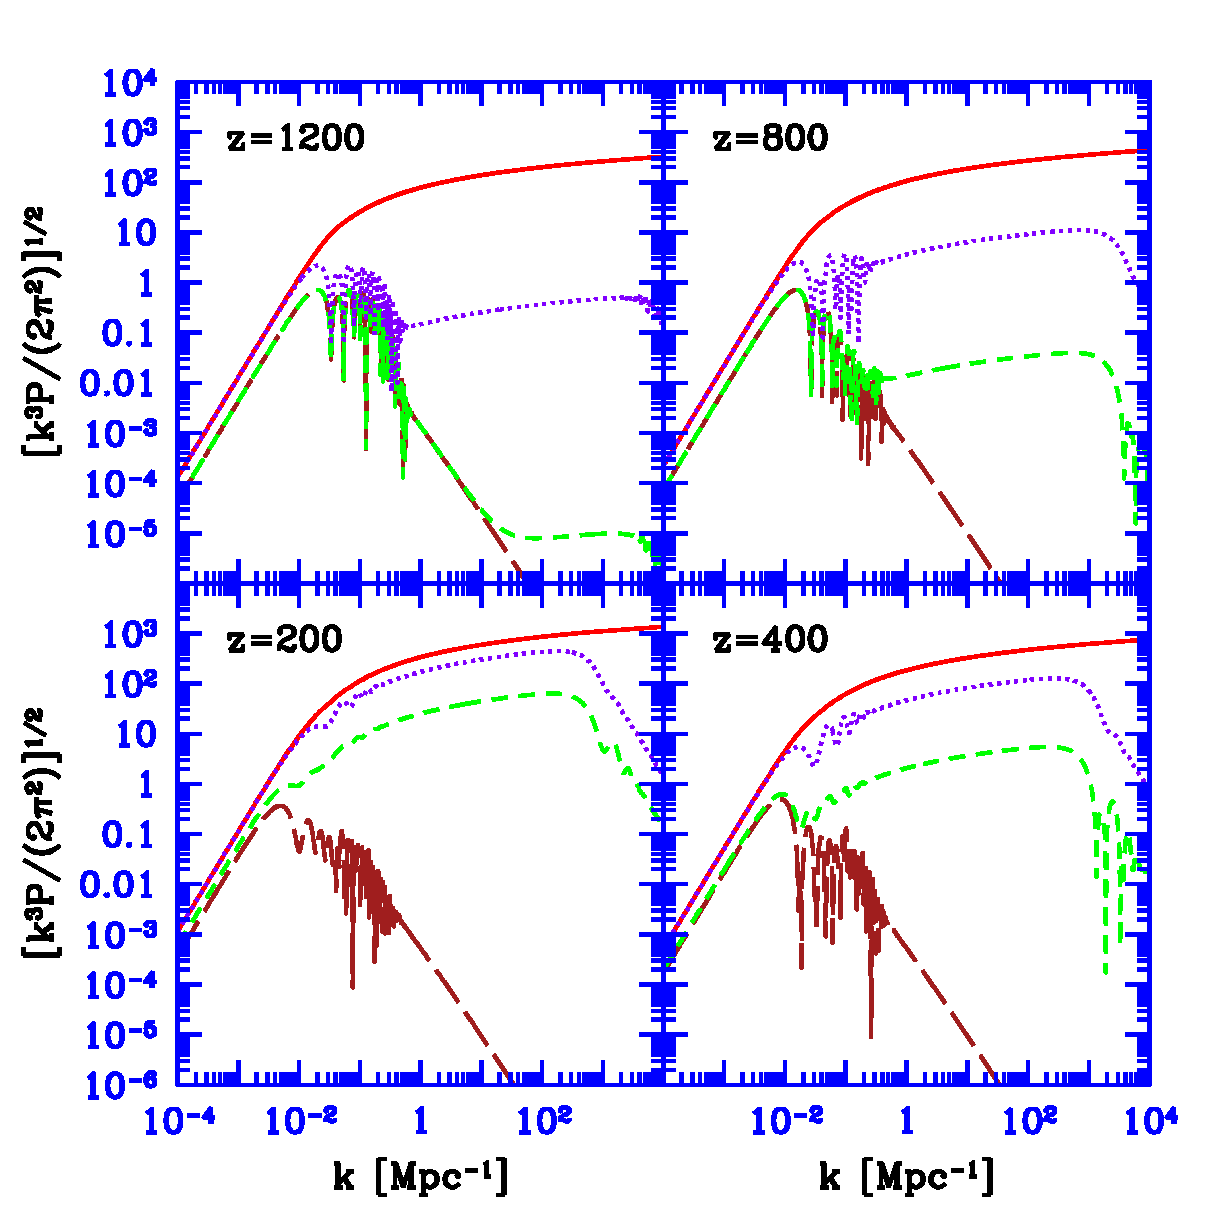
\includegraphics[height=10cm]{Furlanetto_phys/ch2-fullps.eps}}
\caption{Power spectra for density and temperature fluctuations as a function of comoving wavenumber at four different redshifts. The curves show dimensionless power spectra for the CDM density (solid), baryon density (dotted), baryon temperature (short-dashed), and photon temperature (long-dashed). These curves do not include the relative streaming of the baryons and cold dark matter. Reproduced from Naoz, S. \& Barkana, R., ``Growth of linear perturbations before the era of the first galaxies,� \emph{Monthly Notices of the Royal Astronomical Society}, vol. 362, pp. 1047--1053. Copyright OUP 2005.}
\label{fig:nb-pk}
\end{figure}

The solid curve in Figure~\ref{fig:nb-pk} shows the cold dark matter power spectrum at several redshifts during the Dark Ages (taken from \cite{naoz05}). The most obvious feature is the flattening at $k \sim 0.1$~Mpc$^{-1}$, which results from stagnation in the growth of small-scale structure during the radiation era. The power spectrum is otherwise quite simple. However, the 21-cm line will probe the fluctuations in the IGM \emph{gas}, which we will require more physics to understand. 

For example, equation~(\ref{eq:Compton}) describes the evolution of the \emph{mean} IGM temperature.  However, that field actually fluctuates as well, for two reasons \cite{naoz05}.  First, the CMB temperature itself has fluctuations, so each electron will scatter off a different local $T_\gamma$: the power spectrum of the CMB temperature fluctuations is shown by the long-dashed curve in Figure~\ref{fig:nb-pk}. Additionally, the adiabatic expansion term depends on the local density, because gravity slows the expansion of overdense regions and hence decreases the cooling rate (and of course in underdense regions, the cooling accelerates).  Thus, the IGM will be seeded by small temperature fluctuations reflecting its density structure.

To describe these fluctuations, we write $\delta_T$ as the fractional gas temperature fluctuation and $\delta_\gamma$ as the photon density fluctuation (so that $\delta_\gamma = 4 \delta_{T_\gamma}$, the fractional CMB temperature fluctuation). Then the perturbed version of equation~(\ref{eq:Compton}) is 
\begin{equation}
{d \delta_T \over dt} = {2 \over 3} {d \delta_b \over d t} + {x_e(t) \over t_{\rm C}(z)} \left[ \delta_\gamma \left( {\bar{T}_\gamma \over \bar{T}_e} - 1 \right) + {\bar{T}_\gamma \over \bar{T}_e}
(\delta_{T_\gamma} - \delta_T) \right],
\label{eq:deltaT-fluc}
\end{equation} 
where the first term describes adiabatic cooling due to expansion (allowing for variations in the expansion rate) and the second accounts for variations in the rate of energy exchange through Compton scattering (which can result from variations in either the gas or photon temperatures).

Meanwhile, the fluctuations in the baryon temperature affect the baryon density evolution as well.  Equation~(\ref{eq:linper}) implicitly assumed that temperature fluctuations were driven (only) by density fluctuations; allowing a more general relation, we obtain \cite{naoz05}
\begin{equation}
\frac{\partial^2\delta}{\partial t^2}+2 H
\frac{\partial\delta}{\partial t}={3 \over 2} H^2 \left( {\Omega_c
\delta_c + \Omega_b \delta_b} \right) - {k^2 \over a^2} {k_B \bar{T}_e
\over \mu m_H} (\delta_b + \delta_T).
\label{eq:linper-Tfluc}
\end{equation}
 This, together with equations~(\ref{eq:deltaT-fluc}), (\ref{eq:Compton}), and a more precise version of~(\ref{eq:dxedt}) for the temperature and ionized fraction evolution, provide a complete set of equations to trace the density and temperature evolution (modulo one more effect that we will discuss next).  
 
Figure~\ref{fig:nb-pk} shows the resulting power spectra for the dark matter density, baryon density, baryon temperature, and photon temperature perturbations at four different redshifts.  The photon fluctuations are not directly observable, but the others can in principle be probed through the 21-cm line.  The photon perturbations are strongly suppressed on scales below the sound horizon thanks to their large pressure.  Near recombination, the baryonic perturbations are also suppressed on these scales, especially in the temperature, because they interact so strongly with the CMB.  However, after recombination, the baryons fall into the dark matter potential wells,
with their perturbations rapidly growing, and temperature fluctuations also grow thanks largely to the variations in the adiabatic cooling rate.  The turnover at very small scales in the baryonic power spectrum is due to the finite pressure of the gas. 

\subsubsection{Relative Streaming of Baryons and Cold Dark Matter} 

There is one additional effect on the baryonic power spectrum that may provide insight into cosmology during this era: ``streaming" of baryonic matter relative to dark matter \cite{tseliakhovich10}. As a relativistic fluid, CMB photons have a very high pressure that drives acoustic waves throughout that component. While these photons are coupled to the baryons through Compton scattering, they can drag the baryonic component along with them -- it is these acoustic waves in the photon-baryon fluid that we see in CMB fluctuations. Once recombination occurs, the radiation drag force decreases, and the baryons begin to fall into the potential wells of dark matter fluctuations (which have not participated in the acoustic waves). This transition can be seen in the dotted and short-dashed curves in Figure~\ref{fig:nb-pk}. Because the radiation sound speed is $\sim c/\sqrt{3}$, it is near the causal horizon at the time of recombination, corresponding to $\sim 150$~comoving Mpc today, where they can be observed as ``baryon acoustic oscillations" in the matter power spectrum (and, because their physical scale is well-known, used as a standard ruler to measure cosmological parameters). 

%%%%%%%%%%%%%%%%Figure: Velocity power spectrum
\begin{figure}
\centerline{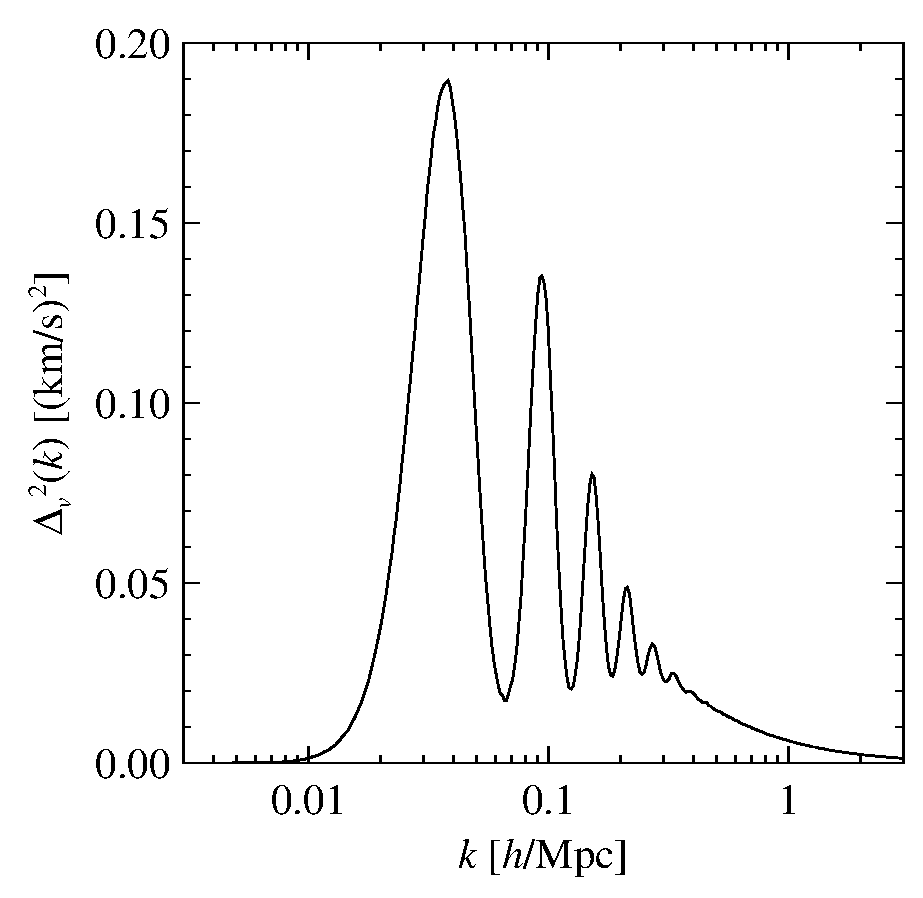
\includegraphics[width=10cm]{Furlanetto_phys/Deltav.eps}}
\caption{The power spectrum of the velocity difference perturbations 
(in units of between baryons and dark matter as a
function of comoving wavenumber $k$ at $z=15$.  Reproduced from N. Dalal, U.-L. Pen, \& U. Seljak. {\it Journal of Cosmology \& Astroparticle Physics} {\bf 2010}, 007. Copyright 2010 IOP Publishing and Sissa Medialab srl. All rights reserved. }
\label{fig:delta_v}
\end{figure}

There is an additional effect relevant to high redshifts, however. Even after the radiation driving becomes ineffective, the baryons are left with a relic velocity imprinted by the pressure force with a root-mean-square ({\it rms}) speed of $v_{\rm bc}\approx 10^{-4}c=30~{\rm km~s^{-1}}$, which decays with redshift as
$1/a$ \cite{tseliakhovich10}. This \emph{streaming velocity} between the baryonic and dark matter components is coherent over very large scales -- comparable to the acoustic scale -- and fades only slowly over time. Figure~\ref{fig:delta_v} shows the variance of the relative velocity perturbations  as a function of the mode wavenumber $k$ at $z=15$. The power is substantial on scales up to the sound horizon at decoupling ($\sim 140$ comoving Mpc), but it declines rapidly at $k>0.5~{\rm Mpc^{-1}}$, indicating that the streaming velocity is coherent over a scale of several comoving Mpc. Therefore, in the rest-frame of small-scale fluctuations (such as those that will eventually collapse into galaxies), the baryons appeared to be moving coherently as a ``wind," which can suppress the formation of the first galaxies \cite{dalal10, fialkov14}, and can result in a standard ruller during the cosmic dawn \cite{munoz19, munoz19-ruler}.

\subsection{The Global 21-cm Signal During the Dark Ages} \label{cos-21cm-dark}

%%%%%%%%%%%%%%%%Figure: Mirocha
\begin{figure}
\centerline{\includegraphics[width=8cm]{dark_ages_lcdm} \includegraphics[width=8cm]{Furlanetto_phys/dapper_prospects_1panel}}
    \caption{\emph{Left:} The Dark Ages 21-cm absorption trough in the standard cosmology. The shape at $z > 30$ is independent of astrophysical sources. \emph{Right:} The black dashed line shows the mean 21-cm brightness temperature (averaged across the sky) in the standard cosmology. The gray contours show schematically the reported EDGES absorption signal \cite{Bowman18}. The solid curves are phenomenological models that invoke extra cooling to match the amplitude of the EDGES signal but that also dramatically affect the Dark Ages absorption trough at $z>50$. Courtesy J. Mirocha, based on calculations in \cite{mirocha19}.}
    \label{fig:sample-histories}
\end{figure}

With the thermal history from Figure~\ref{fig:darkage-thermal}, we can easily calculate the global 21-cm signal throughout the Dark Ages -- without any way of generating a Lyman-$\alpha$ background, the competition between the CMB and particle collisions sets the spin temperature. The left panel of Figure~\ref{fig:sample-histories} shows the result: once the gas temperature begins to fall below the CMB temperature at $z \sim 150$, the 21-cm signal can be seen in absorption. At these early times, the gas is relatively dense and has a high enough temperature for collisional coupling to be substantial, so $T_S \rightarrow T_K$. However, as the gas expands and cools, collisional coupling becomes inefficient, and eventually the spin temperature begins to return to $T_\gamma$. By the time we expect star formation to begin in earnest ($z < 30$), $T_S \approx T_\gamma$, so the 21-cm line is nearly invisible. 

The global 21-cm signal is therefore sensitive to the IGM thermal history, so any process that affects the temperature evolution can also be probed by the 21-cm line. This method provides a particularly powerful probe of non-standard physics because the low gas temperature during this period makes the 21-cm line a sensitive calorimeter of additional heating (or cooling) and/or of an excess radio background over and above the CMB \cite{feng18}.

While many such processes tend to \emph{heat} the IGM and therefore \emph{decrease} the amplitude of the 21-cm signal (e.g. \cite{chen04-decay, furl06-dm,shchekinov07, chuzhoy08}), the recent claim of a detection of a 21-cm absorption feature at 78~MHz ($z \sim 17$) by the EDGES collaboration \cite{Bowman18} has triggered interest in non-standard models that \emph{amplify} the 21-cm signal (though note that the EDGES signal has not yet been independently confirmed, and with such a challenging analysis systematics and foreground contaimnation remain a concern \cite{hills18, draine18, spinelli19, bradley19}). The EDGES feature is more than twice as deep as expected if gas follows the standard thermal history, even if astrophysical sources were able to drive $T_S \rightarrow T_K$ and no X-ray heating had yet occurred. It therefore requires new physics that either \emph{cools} the IGM or \emph{increases} the radio background against which the gas absorbs. A multitude of processes has been proposed to explain the anomalous detection, including dark matter-baryon scattering \cite{munoz15, barkana18, slatyer18, hirano18}, millicharged dark matter \cite{munoz18-cool, berlin18, kovetz18}, axions \cite{moroi18}, neutrino decay \cite{chianese19}, charge sequestration \cite{falkowski18}, quark nuggets \cite{lawson19}, dark photons \cite{jia19}, and interacting dark energy \cite{costa18}, and it has been used to constrain additional exotic processes like dark matter annihilation \cite{cheung19}.

Although the EDGES signal at $z \sim 17$ is very likely past the end of the Dark Ages -- after the first astrophysical sources formed -- the same new physics would have affected the Dark Ages signal. The solid curves in Figure~\ref{fig:sample-histories} illustrate how models that invoke excess cooling to explain the EDGES result (shown schematically by the gray contours) could also greatly amplify the Dark Ages signal. (Here the curves use a phenomenological parameterized cooling model as in \cite{mirocha19}; physically-motivated models will differ in the details.) (Note that the signal still vanishes at $z \sim 30$ because collisional coupling is still inefficient.) In these cases, even though the exotic physics have implications at relatively low redshifts, Dark Ages observations serve to break degeneracies between astrophysics and that new physics.

\subsection{The Power Spectrum During the Dark Ages} \label{cos-21cm-ps}

As we have discussed, maps of 21-cm emission provide a sensitive probe of the power spectrum of density and temperature fluctuations \cite{kleban07, mao08}. Figure~\ref{fig:pritchard-flucs}, from \cite{pritchard12}, shows examples of how modes of the 21-cm fluctuation power spectrum evolve in the standard cosmology. Although the strongest fluctuations occur at $z \sim 10$, when astrophysical sources dominate, the Dark Ages signal are not too far behind: this is because, although the fractional density fluctuations are small at those times, the mean temperature can be relatively large during the absorption era -- even in the standard cosmology.

%%%%%%%%%%%%FIGURE: Power spectrum over time
\begin{figure}
	\centerline{\includegraphics[width=7.5cm]{Furlanetto_phys/pritchard-flucs-color}}
    \caption{ 21-cm fluctuations are substantial during the Dark Ages. The curves show the amplitude of the 21-cm brightness temperature fluctuations at several different wavenumbers from the Dark Ages to low redshifts, in the standard model of cosmology. Red diagonal lines compare these fluctuations to the foreground brightness temperature (from Galactic synchrotron): each scales the foreground by the number shown. Note that exotic cooling scenarios described in \S \ref{cos-21cm-dark} could significantly amplify these fluctuations. From \cite{pritchard12}. Copyright IOP Publishing. Reproduced with permission. All rights reserved.}
    \label{fig:pritchard-flucs}
\end{figure}

The 21-cm power spectrum during the Dark Ages offers several advantages over other probes of the density field. Because they use the cosmological redshift to establish the distance to each observed patch, 21-cm measurements probe three-dimensional volumes --- unlike the CMB, which probes only a narrow spherical shell around recombination. Additionally, the 21-cm line does not suffer from Silk damping (photon diffusion), which suppresses the CMB fluctuations on relatively large scales. The number of independent modes accessible through this probe is therefore \cite{loeb04}
\begin{equation}
N_{\rm 21cm} \sim 8 \times 10^{11} \left( {k_{\rm max} \over 3 \ \mbox{Mpc}^{-1}} \right)^3 \left( {\Delta \nu \over \nu} \right) \left( {1+z \over 100} \right)^{-1/2},
\label{eq:nmax}
\end{equation}
where $\Delta \nu$ is the bandwidth of the observation. The choice of $k_{\rm max}$ --- the smallest physical scale to be probed --- is not obvious. The Jeans length during the Dark Ages corresponds to $k_{\rm max} \sim 1000\ \rm{Mpc}^{-1}$. Accessing these small-scale modes in three dimensions would require an enormous instrument, but our relatively conservative choice in equation~(\ref{eq:nmax}) shows that even a more modest effort provides a massive improvement over the information contained in all the measurable modes of the CMB, $N_{\rm CMB} \sim 10^7$. Moreover, because the density fluctuations are still small at such early epochs, these modes remain in the linear or mildly non-linear regime, allowing a straightforward interpretation of them in terms of the fundamental parameters of our Universe \cite{lewis07}.  

%%%%%%%%%%%%FIGURE: Cosmology dependence
\begin{figure}
	\centerline{\includegraphics[width=9cm, clip=True, trim=0cm 0.8cm 0cm 0cm]{Furlanetto_phys/sample-cosmologies}}
    \caption{The 21-cm power spectrum is a sensitive probe of cosmological parameters. The angular power spectrum of 21-cm fluctuations at $z=55$ in ``standard" cosmologies, varying some of the parameters. The solid and dotted curves use $\Lambda$CDM with the power law index of density fluctuations $n_s=1$ and 0.98; respectively; the short-dashed curve adds a ``running" to the spectral index. The long-dashed curve assumes 10\% of the matter density is in the form of massive neutrinos (with masses 0.4~keV), while the dot-dashed curve assumes warm dark matter with particle masses of 1~keV.  Reprinted figure from Loeb, A. \& Zaldarriaga, M., {\it Phys. Rev. Lett.} {\bf 92}, 21, 211301. Copyright 2004 by the American Physical Society.}
    \label{fig:sample-cos}
\end{figure}

In principle, measurements of the 21-cm power spectrum during the Dark Ages will therefore enable a number of precision cosmological measurements, even within the ``standard" cosmology. For example, because 21-cm fluctuations extend to such small scales, they expand the dynamic range of power spectrum measurements over several orders of magnitude. This is useful for a number of specific cosmological parameters, as illustrated by the curves in Figure~\ref{fig:sample-cos}, but also including the running of the spectral index of the matter power spectrum \cite{mao08}, a key parameter that can test the underlying assumptions of the inflationary paradigm, as well as the total spatial curvature and neutrino masses \cite{mao08}.

The large number of modes is also essential to constraining primordial non-Gaussianity in the cosmological density field, which is another tool for testing  inflationary models. CMB measurements already offer constraints, which can best be improved by larger-volume surveys. However, low-$z$ galaxy surveys suffer from contamination, because nonlinear structure formation also generates non-Gaussianity. The ``clean," small-scale Dark Ages 21-cm field is an excellent opportunity to further constrain the non-Gaussianity  \cite{chen18} -- in principle, 21-cm Dark Ages measurements can test the generic inflationary picture itself \cite{munoz15-ng}. 

The potential insights we have discussed so far are useful within the standard cosmology, but the exotic physics mechanisms discussed in the previous section will inevitably affect the 21-cm power spectrum as well, though the implications have only recently begun to be explored. Most obviously, the power spectrum amplitude is proportional to the square of the mean brightness temperature. But more subtle signatures that depend on the particulars of the physics can also appear. For example, if the cooling is triggered by scattering between the baryons and a fraction of the dark matter that has a modest charge, the scattering rate will be modulated by the relative streaming velocity of dark matter and baryons. Such a model therefore leaves distinct features in the 21-cm power spectrum that trace the velocity structure. The detailed implications of most of these exotic models are mostly unexplored, but any model in which (1) the energy exchange depends on local density, velocity, or temperature; or (2) in which background radio energy deposition is inhomogeneous, should generically leave signatures in the power spectrum. 

\section{Cosmology During the Era of Astrophysics} \label{cos-astro}

Although the Dark Ages offer a clean and powerful testbed to probe cosmology, in practice they will be difficult to explore. Not only do the astrophysical foregrounds become significantly stronger at low frequencies (as shown by the diagonal lines in Figure~\ref{fig:pritchard-flucs}, which increase toward higher redshifts), but Earth's ionosphere also becomes opaque at very low frequencies \cite{datta14}, which may necessitate observations from space or the Moon.

Because the 21-cm background will likely be observed at lower redshifts -- after the first luminous sources have appeared -- we will next consider how cosmological information might be extracted from observations during the Cosmic Dawn. The effects we have already described will also affect the global 21-cm signal and the power spectrum during the later era. However, many astrophysical mechanisms (those described in Chapter~2) also affect the 21-cm background during this era, so the challenge is to separate the cosmological information from the astrophysical. In this section, we shall consider some strategies to do that.

\subsection{Isolating the Matter Power Spectrum} \label{cos-ps}

Conceptually, the simplest method is simply to measure the 21-cm power spectrum and fit simultaneously for both astrophysical and cosmological parameters. We will discuss the practicalities of such fits in Chapter~4, but it will suffice for now to note that it is not a trivial exercise, and adding additional cosmological parameters will be a challenge \cite{clesse12, kern17, park19}. Moreover, the astrophysical effects can be very strong and hence mask any cosmological effects. 

Short of modeling the astrophysics precisely enough to extract cosmology -- a strategy whose potential won't really be known until the astrophysics is better understood\footnote{However, note that recent work has shown that the ionization field may be constructed as a perturbative expansion around the density field in certain regimes, which suggests precision modeling may indeed be possible \cite{mcquinn18, hoffmann19}.} -- the chief hope for isolating the power spectrum is that there exists an era in which astrophysics processes can largely be ignored. This is not an entirely unreasonable expectation. Recall from Chapter~1 that the 21-cm brightness temperature is
\begin{equation}
T_b(\nu) \approx  9\;x_{\rm HI}(1+\delta) \, (1+z)^{1/2}\, \left[1-\frac{T_{\gamma}(z)}{T_S}\right] \, \left[ \frac{H(z)/(1+z)}{d v_\parallel/d r_\parallel} \right] \ \mbox{mK}.
\label{eq:Tb-cos}
\end{equation}
Astrophysical effects determine the neutral fraction $x_{\rm HI}$ and the spin temperature $T_S$, but the other factors -- density and velocity -- are driven by cosmological processes. Thus we can imagine that cosmological information will show up clearly in the power spectrum if, for example, there exists a period in which $T_S \gg T_\gamma$ (so that the temperature effects can be ignored) but in which ionization fluctuations are not yet significant. 

Simple estimates show that such a period is far from impossible -- but also not guaranteed. Reionization requires at least one ionizing photon per baryon, or of order $\sim 10$~eV of ionizing energy released by stars per baryon. Heating the IGM above the CMB temperature -- so that $(1 - T_\gamma/T_S) \approx 1$ requires only $\sim 10^{-2}$~eV (corresponding to a temperature $\sim 100$~K, though only a fraction of the X-ray energy would actually be used to heat the IGM; see \S \ref{xrayheat}). Thus if early sources produce at least $\sim 10^{-3}$ as much energy in X-rays as they do in ionizing photons, heating would occur before reionization -- leaving open the possibility that a period exists in which astrophysics can be ignored. More complex astrophysical processes can also enable such a period as well -- for example, strong photoheating feedback can delay reionization relative to X-ray heating \cite{mesinger13}. Whether this is more than speculation remains uncertain: calibrating the X-ray luminosity of star-forming galaxies to local measurements suggests that the reionization epoch may overlap with the X-ray heating epoch \cite{mirocha17, park19}, but if the EDGES measurement is confirmed, heating must actually occur very early in the Cosmic Dawn, well before reionization is complete.

\subsection{Redshift Space Distortions} \label{cos-redshift-space}

To this point, we have largely ignored the last factor in equation~(\ref{eq:Tb-cos}): the velocity gradient. However, it offers another route to extracting cosmological information. Usually, we expect the fluctuations from the other terms -- density, ionization fraction, Ly$\alpha$ flux, and temperature -- to be  isotropic, because the processes responsible for them have no preferred direction [e.g., $\delta({\bf k}) = \delta(k)$]. However, peculiar velocity
gradients introduce anisotropic distortions through the ``Kaiser effect" \cite{kaiser84}, which emerge because 21-cm observations use the line's observed frequency as a proxy for the distance of the cloud that produced it. 

Consider a spherical overdense region. Because of its enhanced gravitational potential, the region expands less quickly than an average region of the same mass. Therefore, to an observer using redshift as a distance indicator, the apparent \emph{radial} size of the overdense region is smaller than that of the average region. Of course, its transverse size can be measured by its angular extent on the sky so is unaffected by the velocity structure. Thus, to the observer, the spherical region is distorted, appearing larger along the plane of the sky than in the radial direction. An underdense region is distorted in the opposite way: because it expands faster than average, it appears larger in the radial direction than along the plane of the sky. Thus redshift space distortions will \emph{exaggerate} intrinsic density fluctuations, but they do so in an anisotropic way -- making this source of fluctuations separable from others \cite{barkana05-vel, mcquinn06-param}.

To see these effects, we start by labeling the coordinates in redshift space with ${\bf s}$. Assuming that the radial extent of the volume is small, so that the Hubble parameter $H$ is constant throughout the volume, these coordinates are related to the real space ${\bf r}$ by 
\begin{equation} 
{\bf s}({\bf r}) = {\bf r} + {U({\bf r}) \over H}, 
\end{equation} 
where $U({\bf r}) = {\bf v} \cdot \hat{\bf x}$ is the radial component of the peculiar velocity.

Now consider a set of particles with number density $n({\bf r})$ that are biased with respect to the dark matter by a factor $b$. Number conservation demands that the fractional overdensity in redshift space is related to that in real space via $[1 + \delta_s({\bf s})] d^3 {\bf s} = [1 + \delta({\bf r})] d^3 {\bf r}$. The Jacobian of the transformation is \begin{equation}
d^3{\bf s} = d^3{\bf r} \left[ 1 + {U({\bf r}) \over r} \right]^2 \left[ 1 + {dU({\bf r}) \over dr} \right], 
\end{equation} 
because only the radial component of the volume element, $r^2 dr$, changes from real to redshift space.  Thus the density observed in redshift space increases if the peculiar velocity gradient is smaller than the Hubble flow, while the redshift space density will be smaller if the peculiar velocity gradient is larger.  Thus, assuming $|U(r)| \ll Hr$, 
\begin{equation}
\delta_s({\bf r}) = \delta({\bf r}) - \left( {d \over dr} + {2 \over r} \right) {U(r) \over H}.
\label{eq:delta-s}
\end{equation}
Importantly, the peculiar velocity field itself is a function of the dark matter density field, as described qualitatively above. More rigorously, in Fourier space the components of the peculiar velocity ${\bf u}_{\bf k}$ are directly related to those of the density field, because the latter sources the gravitational fluctuations that drive the velocity gradients (e.g., \cite{kaiser84}):
\begin{equation} 
{\bf u}_{{\bf k}} = -i {a H f(\Omega) \over k} \delta_{\bf k} \hat{\bf k},
\label{eq:vpec}
\end{equation} 
where $f(\Omega)$ is a function of the growth rate of cosmological perturbations.  

Equation~(\ref{eq:delta-s}) shows that there are two corrections from the redshift space conversion. To see which of these dominates, consider a plane wave perturbation, $U \propto e^{i {\bf k} \cdot {\bf r}}$. Then the derivative term is $\sim kU/H_0$ while the last term is $\sim U/H_0 r$.  But $r$ is the median distance to the survey volume, and $k$ corresponds to a mode entirely contained inside it, so $k r \gg 1$, and we may neglect the last term.  If we further make the small-angle approximation and make a Fourier transform, so that $\hat{\bf x}$ is also approximately a constant over the relevant volume, the Fourier transform of equation~(\ref{eq:delta-s}) is 
\begin{equation} 
\delta_s({\bf k}) = \delta({\bf k})[ 1 + \beta \mu_{\bf k}^2], 
\end{equation} 
where $\mu_{\bf k} = \hat{\bf k} \cdot \hat{\bf x}$ is the cosine of the angle between the wave vector and the line of sight. Here $\beta = f(\Omega_m)/b$ corrects for a possible bias between the tracers we are studying and the growth rate of dark matter perturbations.  For the case of 21-cm fluctuations in the IGM gas, the bias factor is very close to unity except below the Jeans filtering scale.  

The redshift-space distortions therefore provide an anisotropic \emph{amplification} to the background signal, because only modes along the line of sight are affected. Averaged over all modes, these distortions amplify the signal by a factor $\approx \VEV{(1+ \mu^2)^2} \approx 1.87$ \cite{bharadwaj04-vel}.

For the purposes of extracting cosmological information, the anisotropies are helpful in that they imprint angular structure on the signal, which may allow us to separate the many contributions to the total power spectrum \cite{barkana05-vel}. Brightness temperature fluctuations in Fourier space have the form
\begin{equation}
\delta_{21} =  \mu^{2} \beta \delta + \delta_{\rm iso} 
\label{eq:d21ft}
\end{equation}
where we have collected all the statistically isotropic terms -- including those due to astrophysics -- into $\delta_{\rm iso}$. Neglecting ``second-order" terms (see below) and setting $\beta=1$, the total power spectrum can be written  
\begin{equation}
P_{21}({\bf k}) = \mu^{4} P_{{\delta} {\delta}} + 2 \mu^{2} P_{{\delta}_{\rm iso} {\delta}} + P_{{\delta}_{\rm iso} {\delta}_{\rm iso}}.
\label{eqn:p_polynomial}
\end{equation}
(Here we have written the normal density power spectrum as $P_{\delta \delta}$ for clarity.) By separately measuring these three angular components (which requires, in principle, estimates at just a few values of $\mu$), we can isolate the contribution from density fluctuations $P_{\delta \delta}$. Measuring this component, without any astrophysical contributions, will provide the desired cosmological constraints. 

However, in practice the angular dependence of the power spectrum will not be so simple. To write equation~(\ref{eqn:p_polynomial}), we must neglect ``second-order" terms in the perturbation expansion of the 21-cm field, such as the density and the ionization field perturbations. But the latter is not actually a small term (because, at least in the standard reionization scenarios, $x_{\rm HI}=0$ or 1), so its contributions do not decrease rapidly in higher-order terms \cite{lidz07-ng}. During reionization, these additional terms complicate the angular dependence and will significantly complicate attempts to separate the $\mu^n$ powers during reionization more difficult \cite{mcquinn06-param, shapiro13}. Moreover, if the first H~II regions are highly biased -- thus overlapping the regions with the largest peculiar velocities -- the redshift space distortions can be suppressed \cite{mesinger11, mao12}. The redshift space distortions are also more complicated if the heating and reionization eras overlap \cite{ghara15}.
 
%%%%%%%%%%%%FIGURE: Fialkov streaming
\begin{figure}
	\centerline{\includegraphics[width=9cm, clip=True, trim=0cm 0.6cm 0cm 0.5cm]{Furlanetto_phys/vbc}}
    \caption{The relative streaming velocity between baryons and dark matter can impact the 21-cm power spectrum during the Cosmic Dawn. The solid curves show the time evolution of several example 21-cm power spectra, evaluated at $k \sim 0.1 h$~Mpc$^{-1}$, without including streaming, while the dashed curves show the same scenarios with streaming included. The dotted lines show expected sensitivities of current and future 21-cm radio arrays. Reproduced from Fialkov, A. et al, ``Complete history of the observable 21 cm signal from the first stars during the pre-reionization era," \emph{Monthly Notices of the Royal Astronomical Society}, 437, L36-40. Copyright OUP 2014. }
    \label{fig:streaming}
\end{figure}

\subsection{Indirect Effects of Cosmology on the 21-cm Background} \label{cos-indirect}

Finally, it is also worth noting that cosmological processes can have direct effects on astrophysical sources and hence indirect effects on the 21-cm background. For example, consider warm dark matter. If dark matter has a non-zero velocity dispersion, then it can easily escape from shallow potential wells, suppressing the formation of small dark matter haloes. Because the first phases of galaxy formation occur in small haloes, warm dark matter delays galaxy formation, which in turn delays the formation of Lyman-$\alpha$, X-ray, and ionizing backgrounds and changes the timing (and potentially spatial fluctuations) of the 21-cm background (e.g., \cite{barkana01, yue12,lopezhonorez17}). Of course, this dark matter effect is degenerate with astrophysical processes (for example, strong feedback in small galaxies may also suppress their star formation rates) so requires careful analysis, and other cosmological changes can have qualitatively similar effects (e.g., \cite{yoshida03}), although such effects may be distinct from large swathes of astrophysical parameter space \cite{sitwell14}.

Another example is the interaction between astrophysical processes and the relative streaming between baryons and dark matter. The streaming velocity also suppresses the formation of small baryonic haloes, because a shallow potential well cannot accrete gas traveling by it at sufficiently large velocity. However, unlike in the case of warm dark matter, the streaming effect is spatially variable, so, at least in some circumstances, the streaming effect will imprint spatial structure on the radiation backgrounds and hence on the 21-cm power spectrum \cite{dalal10, fialkov14, munoz19}. Figure~\ref{fig:streaming} shows an example of this effect during the era in which the first stars appear.

Finally, dark matter annihilation offers an other interesting example of the interaction between cosmology and astrophysics. The heating from dark matter annihilation occurs very uniformly. If astrophysically-driven X-ray heating begins within such a pre-heated medium, the associated large-scale peak in the power spectrum occurs in emission rather than absorption, providing a distinct signature for (some) dark matter annihilation scenarios  \cite{evoli14, lopez16}. 

%%%%%%%%%%%%FIGURE: CMB constraints
\begin{figure}
	\centerline{\includegraphics[width=9cm, clip=True, trim=0cm 0cm 0cm 0cm]{Furlanetto_phys/AsTau_w21cm}}
    \caption{Constraints on the amplitude of the primordial power spectrum, $A_s$, and the CMB optical depth to electron scattering, $\tau$. The elongated curves show the current constraints (at 1 and $2\sigma$) from combining the Planck satellite and several other probes. The tighter constraints show the combination with forecasted measurements from HERA, illustrating how the 21-cm measurement of the ionization history substantially improves constraints on other cosmological parameters. Figure based on calculations from \cite{liu16}, provided courtesy A. Liu.}
    \label{fig:cmb}
\end{figure}

\section{21-cm Cosmology in a Larger Context} \label{cos-complementary}

Although the focus of this book is on the 21-cm line itself, it is worth emphasizing that observations of the high-$z$ spin-flip background will ultimately be combined with many other observations. For cosmological measurements, it is therefore useful to understand synergies between the 21-cm background and other probes \cite{liu16, liu16-cmb}. Some of the key advantages of the 21-cm line have already been described: it can probe small physical scales and high-redshifts. Additionally, it can break degeneracies within other probes. Figure~\ref{fig:cmb} shows an example. If the 21-cm line can measure the reionization history, it provides an independent estimate of the CMB optical depth to electron scattering, which is otherwise nearly degenerate with the amplitude of the initial power spectrum -- and thus allow a precision measurement of that parameter.


\bibliographystyle{plain}
\bibliography{Furlanetto_phys/ch3-refs}


\chapter{Inference from the 21cm signal}

\begin{bf}
  \author{Bradley Greig}\\
  
Abstract\\
\end{bf}

The 21cm signal is physics rich and encodes a wealth of astrophysical and cosmological information (refer back to previous chapters here). However, how do we extract this information? This chapter focusses on how we intend to extract the interesting physics from the observed 21cm signal.

Essentially, the problem can be broken down into three parts:
\begin{itemize}
\item[1.] Compressing the observed data into a manageable dataset (i.e. statistic or images) to tease out the interesting physics. Which is the optimal statistic, and what in particular is it optimal for?
\item[2.] An efficient means to model/simulate the 21cm signal
\item[3.] A robust probabilistic framework to compare simulations to observations to extract the physics.
\end{itemize}
\noindent
In this chapter we will focus on each separately, before concluding with the current state of the art in inference of the 21cm signal.

\section{What do we actually measure?}

Ultimately, we observe the brightness temperature fluctuations in the 21cm signal, relative to the background CMB temperature. In effect, we observe $\delta T_{b,\rm 21cm}(\nu,\mathbf{x})$, dependant on the observed frequency (line of sight distance) and the 2D angular position on the sky. Interferometric experiments (e.g.) enable us to access the full 3D information of the 21cm signal. Global experiments on the other hand average out the brightness temperature over the entire sky, compressing the information into a single average brightness as a function of frequency.

Once we have a measurement of this 3D 21cm signal, we are free to compress the data in an innumerable number of ways. We can extract single 2D tomographic images of the differential brightness temperature as a function of redshift (frequency) enabling us to be able to directly observe the topology of the neutral and ionised gas during reionisation. Alternatively we can average out the 3D information either spatially or in frequency to maximise the signal to noise in a certain regime to maximise certain astrophysical processes and features expected during reionisation.

\section{Optimal methods for extracting the astrophysics and cosmology from the 21cm signal}

To infer the interesting astrophysics and cosmology from the observational data, we need a way to characterise the spatially and time varying 21cm signal. The signal is weak, therefore we likely will need to compress the data in some way to tease out the interesting physics from the noise.

Here, list a variety of known ways in which can be used to extract information about the 21cm signal. This will include both imaging and statistical techniques. For each, provide a brief discussion about the method (i.e. what it is) and then what leverage it provides in regard to the astrophysics etc. and what specific features are useful \textbf{(this may marginally overlap with Jordan's section on Predictions and Challenges)}. At various points in this section, can refer back to previous chapters when specific physics is being referred to. For example, if a specific statistic is sensitive to a certain population of sources or an epoch of history, refer back to the appropriate section in the previous chapters.

This should be a considerable more in-depth discussion that what is covered in Jordan's and Jonathan Pritchard's chapters. Need to gauge the overlap between these chapters.

\textbf{Need to work in Adrian Liu's paper highlighting the importance of knowing $\tau$ for precision recovery of cosmology}

\subsection{Minkowski functionals}

Compresses the information down into a single number, which can describe the connectedness and overall topology of the 21cm signal. Cite Zaroubi, also a recent arXiv paper (Chen maybe).

\subsection{Global signal}

Describes the entire globally averaged history of the 21cm signal. Turning points/features within the signal can be used to disentangle information about sources etc. Can also throw in some discussion regarding EDGES/DM, i.e. fundamental cosmology + astrophysics. \textbf{How much overlap is there going to be between this and Jordan/Jonathan Pritchard's chapters.?}

There are a variety of papers investigating the global signal. Could be a few different ways to use the signal to extract information. \textbf{This may overlap with Jordan's chapter on predictions and challenges.}

\subsection{Power spectrum}

The main goto statistic to describe the signal. Sensitive to a vast array of astrophysics. \textbf{This may overlap with Jordan's chapter on predictions and challenges.}

However, doesn't fully describe the signal. Power spectrum is a Gaussian statistic, the signal is inherently non-Gaussian. Therefore information loss.

This should focus only on the 3D spherically averaged 21cm PS. Can mention that the 2D cylindrically averaged PS can in principle also be used, and why it would be useful.

\subsection{Skewness/Kurtosis/PDFs etc.}

A means to measure the non-Gaussianity of the signal, however, compresses the information as it is a scale independent quantity. Useful for describing topology and evolution of the signal. Has certain characteristic features of interest. See Catherine's paper and others.

\subsection{Bispectrum}

A scale dependant measure of the non-Gaussianity of the 21cm signal. Superior to both the power spectrum and skewness etc.. More complicated to visualise/understand. Has been used to describe the EoR quite extensively. Discuss the variety of configurations and their utility/usefulness. See Suman's, and other publications.

\subsection{Wavelets}

An alternative to simply Fourier transforming the data, a family of wavelets can be used to transform the 21cm data to a more useful basis. For example, the Morlet transform allows the transform to be localised both in frequency and in space, improving over the Fourier transform which can only be localised in one or the other. 

In theory, it should contain similar, if not more information that the power spectrum, as it can disentangle line-of-sight effects better. See Cath's paper.

\subsection{Individual bubbles}

Images will provide a direct tangible link to the process of reionisation. Revealing exactly where ionising bubbles are, and thus where to look for the sources responsible for the bubble creation. 

However, bubble identification will become rather problematic, as it is the differential brightness that is observed, not the raw brightness temperature. Need smart/sophisticated approaches to search and characterise the signal.

Look at individual regions of interest, i.e. around a bright QSO or large number of galaxies. 

Matched filters etc., are useful for finding/detecting isolated bubbles

\subsection{Stacked images}

May be difficult to detect individual objects, instead, one could stack 21cm spectra centred on known galaxies. See Paul Geil's paper.

Border's on potential discussions of synergies. Requires known locations of ionising sources with precise redshifts and positions of the sky. JWST/WFIRST. Is there 

\subsection{Bubble size distributions/statistics}

Constructing a statistical distribution of the ionised bubbles through redshift can reveal information about the size and number of galaxies responsible for reionisation (also the production rate of the ionising photons).

Techniques to recover statistical distributions are for example Sambit's super pixels stuff. Need to look at Koki's granulometry stuff to see where that sits in this context.

\subsection{Other statistics}

Are there other statistics that I have overlooked/forgotten. Need to do a search of the literature to ensure I have covered everything.

\section{Efficient methods to model/simulate the 21cm signal}

Ideally we want to use the largest, most physically accurate simulations to match the observed 21cm signal. However, this is not practical. Instead, we must come up with methods to compensate accuracy for efficiency.\\
\\
Originally I envisaged this section to go as follows
\begin{itemize}
\item Discuss briefly that numerical simulations are great but too computationally expensive
\item Highlight semi-numerical/analytic simulations as fitting the bill by being faster etc.
\item Then discuss alternatives (i.e. emulators).
\end{itemize}
This will need to be re-worked given Jordan's plan to discuss this. I haven't yet thought of a logical plan to motivate this. I guess one way would be to concatenate it into just a simulation section and briefly summarise what was discussed in Jordan's chapter (which is a couple of chapters ago, so might be appropriate to do so). It's less obvious to move into discussing emulators in the absence of motivating the need for them by highlighting the complications of simulations in general.

\subsection{Numerical simulations}

Ideally, use large, numerical simulations to make a realisation which matches observation. Want to include as much physics as possible into these simulations. Doing so, comes at a serious cost. Simulating the 21cm signal is complicated! Brief summary on the required dynamic range. Briefly highlight the expensive nature of these simulations, Hydrodynamics, radiative transfer etc. Quickly becomes computationally prohibitive to run more than a couple of realisations. \textbf{Jordan's section (Modelling Tools) will likely cover most if not all of this}.

\subsection{Semi-numerical/analytic models of the 21cm signal}

Enter semi-numerical approaches, which broadly encapsulate the global average quantities of reionisation and the cosmic dawn and reproduce morphologically similar realisations of the 3D structure. The advantage here is that the computational costs are drastically reduced (orders of magnitude less). \textbf{Jordan's section (Modelling Tools) will likely cover most if not all of this}.

\subsection{Intelligent sampling of the parameter space}

Running simulations to span all of the allowed parameter space may be too computationally intensive. However, perhaps we can make intelligent assumptions/guesses about how many simulations to run, and on a specific area of physics to focus on. Some of the concepts here may overlap slightly with the Emulator section below. This sampling was discussed in one of Benoit's recent papers.

\subsection{Emulators}

An alternative to directly running a simulation to estimate some astrophysical statistic/model, one can instead construct a function which estimates what the statistical signal should be, given some astrophysical or cosmological parameter set. This is what is referred to as an emulator. Using simulations, a generator function is constructed which can approximate the statistics of the signal. Results in multiple orders of magnitude improvement in computational speed as no new simulations are required. However, it can only approximate statistics, it does not generate 3D simulations. 

Developing an emulator benefits from efficient parameter space approaches, as it minimises the size of the database required to construct the emulator. There are a variety of approaches to consider when attempting to minimise the sampling of the astrophysical parameter space. For example Latine-Hypercube, Gaussian processes... Can briefly discuss each method, and a few recent papers that explore methods to do this

There are numerous machine learning approaches to construct an emulator.

Discuss Nick Kern's of 21cmFAST and Cohen's global signal one of Anastasia's code.

\subsection{Characterising our ignorance}

We are fully aware that semi-numerical approaches are inaccurate at 10s of per cent level. Additionally, they oversimplify/completely ignore the underlying astrophysical properties. However, if the global quantities (observables such as luminosity functions etc.) can still be reproduced within agreement, we can develop an understanding of how one might map from a semi-numerical simulation, to a more realistic simulation. Basically, tell the large, computationally expensive simulation where exactly to look in the region of parameter space.

Using summary statistics and globally average observables, we can develop a means to calibrate one simulation to mimic the outputs of another. In other words, develop a bias or functional form to smooth out uncertainties from one simulation to mimic the results of a more detailed simulation.

Describe ongoing attempts to quantify this. i.e. use luminosity functions to calibrate simulations, apply redshift corrections to deal with photon non-conservation etc.

These correction factors etc., will be crucial for inferring astrophysics and cosmology from the 21cm signal


\section{Inference methods for 21cm}

Having discussed methods to model/simulate the 21cm signal, now need to shift focus to methods to infer information about the astrophysics/cosmology from the 21cm signal.

\subsection{Fisher Matrices}

Simplest method, which takes derivatives with respect to model parameters of a functional form (i.e. a 21cm statistical signal) to infer parameter constraints. Effectively, exploits how sensitive the 21cm signal is to specific parameters. Limiting assumption include Gaussianity etc.

Successfully used for cosmology

\subsection{Bayesian MCMC}

Significantly more robust method to parameter inference. Outline Bayes' theorem. Highlight that this basically boils down to exploring by random walks, using a likelihood function and priors to accept/penalise regions of parameter space. Very useful for recovering constraints. Again, successfully used in Cosmology etc.

Describe its use in the context of 21cm. Introduce 21CMMC, and a couple of other codes that use MCMC (Sultan's simfast21, Jordan's global signal, Geraint's MCMC, Simon's Mhysa). Highlight that 21CMMC is the only direct MCMC. Emphasise that techniques such as emulators can be coupled with MCMC to improve overall computational efficiency at the cost of some further inaccuracies.

\subsection{Nested sampling and model inference}

We have a wide variety of simulations, each with their own strength's and weaknesses. In principle, various models/simulations/physical prescriptions can be discriminated against using model selection or inference. Related to MCMC, nested sampling can focus on model selection rather than simply astrophysical recovery. Can refer to Tom Binnie's recent paper.

\subsection{Neural Networks}

Instead of using MCMC to recover parameters from statistics, we can use the full 2/3D images of the 21cm signal with neural networks. One can construct a database of simulations and extract the 21cm signal to construct a neural network. This network can then learn an large number of properties, i.e. how changes in the topology are affected by astrophysical parameters etc. Using this technique one can directly convert from an observed 2D image to the underlying astrophysics. Like emulators, the application of the network is extremely quick. Downsides are parameter errors etc. and in some sense physical intuition. It tells you an answer, but not why.

Simulated images of the 21cm signal have already been used to infer astrophysical and cosmological constraints. For example with convolutional networks (e.g Nicolas or Paul La Plante). Discuss other machine learning approaches.



\iffalse

Lorem ipsum dolor sit amet, consectetur adipiscing elit. Duis eu egestas erat. Maecenas tincidunt lacinia tincidunt. Mauris id lectus nec neque feugiat condimentum vitae at diam. In vel orci nunc, non commodo mauris. Vivamus ipsum enim, vulputate quis pharetra non, molestie quis felis. Vivamus porttitor placerat turpis at accumsan. Nunc tortor velit, faucibus a rhoncus nec, blandit non elit. Nam consectetur lectus eu nisi blandit dapibus rhoncus dui tempus. Mauris fermentum dolor vel ipsum vulputate sit amet ultricies tortor lacinia. Donec ut nibh erat. Morbi nec mi ante. Integer nec vestibulum diam. Donec tincidunt pellentesque quam, ut interdum mauris venenatis condimentum. Nam condimentum, augue in aliquet gravida, neque dui elementum eros, id semper eros purus sed felis. Curabitur in justo sit amet sapien ultrices hendrerit at quis nibh. Quisque iaculis pulvinar tincidunt. 
\begin{eqnarray}
C(12) &= &\left[\overrightarrow{\pi}\cdot\overrightarrow{\phi}(x+r)\right] \nonumber \\ 
&\approx& 1-\mathrm{const}\frac{r^2}{L^2}\int_r^L\frac{x\rmd x}{x^2} + \cdots \nonumber  \\
&\approx& 1-\mathrm{const}\frac{r^2}{L^2}\ln\frac{x\rmd x}{x^2} + \cdots .\label{brokenlongeqn}
\end{eqnarray}

Aenean tellus risus, porta sit amet porta vitae, tincidunt ut felis. Class aptent taciti sociosqu ad litora torquent per conubia nostra, per inceptos himenaeos. Vestibulum ante ipsum primis in faucibus orci luctus et ultrices posuere cubilia Curae; Phasellus pulvinar placerat velit auctor egestas. Vivamus euismod fringilla tincidunt. Sed ut magna felis, id sollicitudin nunc. Quisque a dui eu erat consectetur egestas a quis justo. Aenean euismod congue diam, vel posuere urna fermentum sit amet. Lorem ipsum dolor sit amet, consectetur adipiscing elit. Mauris faucibus lacus eget est mollis auctor. Donec at nibh ligula, et posuere massa. Phasellus quis leo diam \cite{diamantaras1996pcn}.
Donec aliquam blandit risus, eu venenatis ante euismod eu. Curabitur cursus justo id arcu condimentum feugiat. Integer sapien urna, vulputate et adipiscing nec, convallis et justo. Suspendisse in ipsum at felis ornare interdum \cite{tulone2006pts},

\begin{figure}[]
\begin{center}
\includegraphics[width=0.5\textwidth]{Greig/01x01-eps-converted-to}
\end{center}
\caption{This is figure 1 in chapter 1.}
\end{figure}

\paragraph{Cras adipiscing} sagittis nunc vel luctus. Suspendisse volutpat augue quis erat semper consequat dignissim tellus euismod. Morbi hendrerit, tellus id aliquam iaculis, nibh leo tincidunt eros, vitae varius ligula felis in mi.

\begin{table}
\caption{Greek Letters.}
\begin{center}
\begin{tabular}{llllllll}
\hline
$\alpha $  & $ \beta $  & $ \gamma $  & $ \delta $  & $ \epsilon $  & $ \varepsilon $  & $ \zeta $  & $ \eta $ \\
 $ \theta $  &  $ \vartheta $  &  $ \gamma $  &  $ \kappa $  &  $ \lambda $  &  $ \mu $  &  $ \nu $  &  $ \xi $ \\
 $ o $  &  $ \pi $  &  $ \varpi $  &  $ \rho $  &  $ \varrho $  &  $ \sigma $  &  $ \varsigma $  &  $$ \\
 $ \tau $  &  $ \upsilon $  &  $ \phi$ &  $ \varphi $  &  $ \chi $  &  $ \psi $  &  $ \omega$  &  $ $ \\
 &  &  &  &  &  &  & \\
$ \Gamma $  & $ \Delta $  & $ \Theta $  &  $ \Lambda $  &  $ \Xi $  &  $ \Pi $  &  $ \Sigma $  & $ \Upsilon $ \\
 $ \Phi$ &  $ \Psi $  &  $ \Omega $  &  &  &  &  &\\
\hline
\end{tabular}
\end{center}\end{table}

\begin{figure}[]
\begin{center}

\includegraphics[width=0.6\textwidth]{Greig/01x02}
\end{center}
\caption{This is figure 2 in chapter 1.}
\end{figure}

\fi

\bibliographystyle{plain}
\bibliography{Greig/References}



\chapter{Observational strategies: power spectra and images}

\begin{bf}
  \author{Gianni Bernardi (INAF-IRA)}\\
  
Abstract\\

This chapter reviews the basics of radio interferometry (van-Citter-Zernike theorem, uv-coverage, image formation calibration) and how they are linked to the measurements of the 21-cm power spectrum and its tomography 
\end{bf}


\section{Chapter layout}

\begin{itemize}
\item review of basics of interferometry: van-Citter-Zernike theorem, $uv$-coverage, image formation;
\item from visibilities to power spectra (in particular the delay transform approach - some overlap with Trott's chapter);
\item interferometric calibration: impact on foreground subtraction, calibration errors redundant calibration;
\item array design: power spectrum vs imaging, minimmum vs maximum redundancy - some overlap with Trott's chapter?;
\item impact of calibration errors on power spectra;
\item ionospheric impact/calibration;
\item 21-cm image tomography;  
\end{itemize}

\section{Interferometry overview}

The Van Cittert-Zernike theorem expresses the fundamental relationship between the sky spatial brightness (or brightness distribution) $I$ and the quantity measured by an interferometer, i.e. visibility $V$ \citep{TMS}:
\begin{equation}
V_{ij} ({\bf b}, \lambda) = \int_\Omega {\tilde I} (\hat{\sigma}, \lambda) \, e^{-2 \pi i {\bf b} \cdot {\hat \sigma}} d {\bf \sigma},
\label{eq:1}
\end{equation}
where ${\bf b}$ is the baseline vector that separates between antenna $i$ and $j$ and $\hat{sigma}$ is the observing direction (see Figure ???). The baseline vector is here specified in wevelengths, i.e. ${\bf b} = \frac{{\bf b_{\rm m}}}{\lambda}$, where ${\bf b_{\rm m}}$ is the baseline vector expressed in meters and $\lambda$ is the observing wavelength.
The sky brightness distribution does not enter directly in equation~\ref{eq:1}, but filtered by the antenna primary beam response $A$ that depends upon the direction in the sky and the wavelength, i.e. ${\tilde I} = A  \, I$. The response of the primary beam attenuates the sky emission away from the pointing direction, effectively reducing the field of view $\theta$ of the instrument. Generally speaking, the size of the field of view is essentially given by the antenna diamater $D$: 
\begin{equation}
\theta \approx \frac{\lambda}{D}.
\label{eq:2}
\end{equation}
The integral of equation~\ref{eq:1} is normally taken over the source size $\Omega$. Equation~\ref{eq:1} is often re-written in a different coordinate system, i.e. the components of the baseline vector $(u,v,w)$ and the reciprocal $(l,m,n)$, where $(l,m)$ are the coordinates in the plane on the sky tangent to the observing direction $n$ \citep[for further details on coordinate systems see][]{TMS}. Using this different coordinate system, equation~\ref{eq:1} becomes:
\begin{equation}
V_{ij} (u,v,w, \lambda) = \int_\Omega {\tilde I} (\hat{\sigma}, \lambda) \, e^{-2 \pi i (ul + vm + wn} dl \, dm \, dn,
\label{eq:3}
\end{equation}
{\bf (GB: fix the above equation)}...

Although low frequency radio observations are intrinsically wide-field, for the purpose of studying the 21~cm observables, we can reduce equation~\ref{eq:3} to a two dimensional Fourier transform:
\begin{equation}
V_{ij} (u,v, \lambda) = \int_\Omega {\tilde I} (\hat{\sigma}, \lambda) \, e^{-2 \pi i (ul + vm} dl \, dm.
\label{eq:4}
\end{equation}
Equation~\ref{eq:4} indicates that an interferometer measures the two dimensional Fourier transform of the spatial sky brightness distribution.



%Lorem ipsum dolor sit amet, consectetur adipiscing elit. Duis eu egestas erat. Maecenas tincidunt lacinia tincidunt. Mauris id lectus nec neque feugiat condimentum vitae at diam. In vel orci nunc, non commodo mauris. Vivamus ipsum enim, vulputate quis pharetra non, molestie quis felis. Vivamus porttitor placerat turpis at accumsan. Nunc tortor velit, faucibus a rhoncus nec, blandit non elit. Nam consectetur lectus eu nisi blandit dapibus rhoncus dui tempus. Mauris fermentum dolor vel ipsum vulputate sit amet ultricies tortor lacinia. Donec ut nibh erat. Morbi nec mi ante. Integer nec vestibulum diam. Donec tincidunt pellentesque quam, ut interdum mauris venenatis condimentum. Nam condimentum, augue in aliquet gravida, neque dui elementum eros, id semper eros purus sed felis. Curabitur in justo sit amet sapien ultrices hendrerit at quis nibh. Quisque iaculis pulvinar tincidunt. 
%\begin{eqnarray}
%C(12) &= &\left[\overrightarrow{\pi}\cdot\overrightarrow{\phi}(x+r)\right] \nonumber \\ 
%&\approx& 1-\mathrm{const}\frac{r^2}{L^2}\int_r^L\frac{x\rmd x}{x^2} + \cdots \nonumber  \\
%&\approx& 1-\mathrm{const}\frac{r^2}{L^2}\ln\frac{x\rmd x}{x^2} + \cdots .\label{brokenlongeqn}
%\end{eqnarray}
%
%Aenean tellus risus, porta sit amet porta vitae, tincidunt ut felis. Class aptent taciti sociosqu ad litora torquent per conubia nostra, per inceptos himenaeos. Vestibulum ante ipsum primis in faucibus orci luctus et ultrices posuere cubilia Curae; Phasellus pulvinar placerat velit auctor egestas. Vivamus euismod fringilla tincidunt. Sed ut magna felis, id sollicitudin nunc. Quisque a dui eu erat consectetur egestas a quis justo. Aenean euismod congue diam, vel posuere urna fermentum sit amet. Lorem ipsum dolor sit amet, consectetur adipiscing elit. Mauris faucibus lacus eget est mollis auctor. Donec at nibh ligula, et posuere massa. Phasellus quis leo diam \cite{diamantaras1996pcn}.
%Donec aliquam blandit risus, eu venenatis ante euismod eu. Curabitur cursus justo id arcu condimentum feugiat. Integer sapien urna, vulputate et adipiscing nec, convallis et justo. Suspendisse in ipsum at felis ornare interdum \cite{tulone2006pts},
%
%\begin{figure}[]
%\begin{center}
%\includegraphics[width=0.5\textwidth]{Bernardi/01x01-eps-converted-to}
%\end{center}
%\caption{This is figure 1 in chapter 1.}
%\end{figure}
%
%\paragraph{Cras adipiscing} sagittis nunc vel luctus. Suspendisse volutpat augue quis erat semper consequat dignissim tellus euismod. Morbi hendrerit, tellus id aliquam iaculis, nibh leo tincidunt eros, vitae varius ligula felis in mi.
%
%\begin{table}
%\caption{Greek Letters.}
%\begin{center}
%\begin{tabular}{llllllll}
%\hline
%$\alpha $  & $ \beta $  & $ \gamma $  & $ \delta $  & $ \epsilon $  & $ \varepsilon $  & $ \zeta $  & $ \eta $ \\
% $ \theta $  &  $ \vartheta $  &  $ \gamma $  &  $ \kappa $  &  $ \lambda $  &  $ \mu $  &  $ \nu $  &  $ \xi $ \\
% $ o $  &  $ \pi $  &  $ \varpi $  &  $ \rho $  &  $ \varrho $  &  $ \sigma $  &  $ \varsigma $  &  $$ \\
% $ \tau $  &  $ \upsilon $  &  $ \phi$ &  $ \varphi $  &  $ \chi $  &  $ \psi $  &  $ \omega$  &  $ $ \\
% &  &  &  &  &  &  & \\
%$ \Gamma $  & $ \Delta $  & $ \Theta $  &  $ \Lambda $  &  $ \Xi $  &  $ \Pi $  &  $ \Sigma $  & $ \Upsilon $ \\
% $ \Phi$ &  $ \Psi $  &  $ \Omega $  &  &  &  &  &\\
%\hline
%\end{tabular}
%\end{center}\end{table}
%
%\begin{figure}[]
%\begin{center}
%
\includegraphics[width=0.6\textwidth]{Bernardi/01x02}
%\end{center}
%\caption{This is figure 2 in chapter 1.}
%\end{figure}
%
%
\bibliographystyle{plain}
\bibliography{Bernardi/References}



\chapter{Foregrounds}

\begin{bf}
  \author{Emma Chapman (Imperial College London), Vibor Jelić, (Ruđer Bošković Institute)}\\
  
Abstract\\
\end{bf}

This chapter discusses some important things


\section{A Section}

Lorem ipsum dolor sit amet, consectetur adipiscing elit. Duis eu egestas erat. Maecenas tincidunt lacinia tincidunt. Mauris id lectus nec neque feugiat condimentum vitae at diam. In vel orci nunc, non commodo mauris. Vivamus ipsum enim, vulputate quis pharetra non, molestie quis felis. Vivamus porttitor placerat turpis at accumsan. Nunc tortor velit, faucibus a rhoncus nec, blandit non elit. Nam consectetur lectus eu nisi blandit dapibus rhoncus dui tempus. Mauris fermentum dolor vel ipsum vulputate sit amet ultricies tortor lacinia. Donec ut nibh erat. Morbi nec mi ante. Integer nec vestibulum diam. Donec tincidunt pellentesque quam, ut interdum mauris venenatis condimentum. Nam condimentum, augue in aliquet gravida, neque dui elementum eros, id semper eros purus sed felis. Curabitur in justo sit amet sapien ultrices hendrerit at quis nibh. Quisque iaculis pulvinar tincidunt. 
\begin{eqnarray}
C(12) &= &\left[\overrightarrow{\pi}\cdot\overrightarrow{\phi}(x+r)\right] \nonumber \\ 
&\approx& 1-\mathrm{const}\frac{r^2}{L^2}\int_r^L\frac{x\rmd x}{x^2} + \cdots \nonumber  \\
&\approx& 1-\mathrm{const}\frac{r^2}{L^2}\ln\frac{x\rmd x}{x^2} + \cdots .\label{brokenlongeqn}
\end{eqnarray}

Aenean tellus risus, porta sit amet porta vitae, tincidunt ut felis. Class aptent taciti sociosqu ad litora torquent per conubia nostra, per inceptos himenaeos. Vestibulum ante ipsum primis in faucibus orci luctus et ultrices posuere cubilia Curae; Phasellus pulvinar placerat velit auctor egestas. Vivamus euismod fringilla tincidunt. Sed ut magna felis, id sollicitudin nunc. Quisque a dui eu erat consectetur egestas a quis justo. Aenean euismod congue diam, vel posuere urna fermentum sit amet. Lorem ipsum dolor sit amet, consectetur adipiscing elit. Mauris faucibus lacus eget est mollis auctor. Donec at nibh ligula, et posuere massa. Phasellus quis leo diam \cite{diamantaras1996pcn}.
Donec aliquam blandit risus, eu venenatis ante euismod eu. Curabitur cursus justo id arcu condimentum feugiat. Integer sapien urna, vulputate et adipiscing nec, convallis et justo. Suspendisse in ipsum at felis ornare interdum \cite{tulone2006pts},

\begin{figure}[]
\begin{center}
\includegraphics[width=0.5\textwidth]{Chapman_Jelic/01x01-eps-converted-to}
\end{center}
\caption{This is figure 1 in chapter 1.}
\end{figure}

\paragraph{Cras adipiscing} sagittis nunc vel luctus. Suspendisse volutpat augue quis erat semper consequat dignissim tellus euismod. Morbi hendrerit, tellus id aliquam iaculis, nibh leo tincidunt eros, vitae varius ligula felis in mi.

\begin{table}
\caption{Greek Letters.}
\begin{center}
\begin{tabular}{llllllll}
\hline
$\alpha $  & $ \beta $  & $ \gamma $  & $ \delta $  & $ \epsilon $  & $ \varepsilon $  & $ \zeta $  & $ \eta $ \\
 $ \theta $  &  $ \vartheta $  &  $ \gamma $  &  $ \kappa $  &  $ \lambda $  &  $ \mu $  &  $ \nu $  &  $ \xi $ \\
 $ o $  &  $ \pi $  &  $ \varpi $  &  $ \rho $  &  $ \varrho $  &  $ \sigma $  &  $ \varsigma $  &  $$ \\
 $ \tau $  &  $ \upsilon $  &  $ \phi$ &  $ \varphi $  &  $ \chi $  &  $ \psi $  &  $ \omega$  &  $ $ \\
 &  &  &  &  &  &  & \\
$ \Gamma $  & $ \Delta $  & $ \Theta $  &  $ \Lambda $  &  $ \Xi $  &  $ \Pi $  &  $ \Sigma $  & $ \Upsilon $ \\
 $ \Phi$ &  $ \Psi $  &  $ \Omega $  &  &  &  &  &\\
\hline
\end{tabular}
\end{center}\end{table}

\begin{figure}[]
\begin{center}

\includegraphics[width=0.6\textwidth]{Chapman_Jelic/01x02}
\end{center}
\caption{This is figure 2 in chapter 1.}
\end{figure}

\section{Foreground Mitigation}
%%% COMMENTED OUT TEXT IS PROBABLY IRRELEVANT DUE TO PREVIOUS CHAPTERS %%%
%Current and future efforts to provide direct observational insight into the Epoch of Reionization have largely focused on detecting the 21-cm radiation emitted by the neutral hydrogen pervading the Universe at high redshifts. At lower redshifts when the first ionizing sources have begun to ionize bubbles in the neutral hydrogen, the 21-cm signal is diminished until, as those bubbles overlap and entirely ionize the Universe, the 21-cm signal depletes entirely. 

The 21-cm signal emitted by high-redshift neutral hydrogen provides a window into the Epoch of Reionization (EoR), but it is a window that is obscured by layers of foregrounds. Terrestrially, radio frequency interference (RFI) from any human-made sources of radio transmission, such as wind turbines, leads to the necessary excision of frequency channels using a flagging technique (e.g. \citet{Prasad2012ExA....33..157P,Offringa2012}). The number of channels excised is significant, around 1$\%$ of channels of data for MWA and LOFAR \citep{Offringa2019MNRAS.484.2866O,Offringa2015PASA...32....8O}. Without careful mitigation in the calibration, imaging and diffuse foreground removal stages, RFI excision can result in an excess power that scales with the number of excised channels and does not integrate down with time, significantly dominating over the cosmological 21-cm signal by 1-2 magnitudes \citep{Offringa2019MNRAS.484.2866O}. Extra-terrestrially, there exist a multitude of foregrounds which dominate all frequencies of observation and so more subtle methods than excision are required. This part of the chapter discusses the development and current use of Galactic and extragalactic foreground mitigation methods in Epoch of Reionization 21-cm experiments.


\subsection{Foreground Mitigation in the Data Analysis Pipeline}
\subsubsection{Bright Source Removal}
The first stage of foreground removal involves mitigating the effect of the very brightest sources on the sky: the point sources and extended sources. Bright source removal often comes under the umbrella of calibration as opposed to foreground mitigation however we will briefly summarize the process here. For example, the MWA real-time system (RTS) \citep{Mitchell2008ISTSP...2..707M} carries out sequential bright source `peeling' on the visibilities, tracking a few hundred of the brightest sources and comparing to a sky model constructed from existing catalogues and MWA observations \citep{Carroll2016MNRAS.461.4151C}. The gains are calibrated on the strongest source, before that source is peeled (subtracted) from the data, and the next strongest source is used to refine the calibration, and so on until it is deemed that enough bright sources have been removed, usually a few hundred to a thousand at most. The other MWA calibration pipeline, Fast Holographic Deconvolution (FHD) \citep{Sullivan2012ApJ...759...17S}, uses the MWA extragalactic catalogue GLEAM \citep{HW2017MNRAS.464.1146H} to calibrate gains, modelling all sources out to 1$\%$ beam level in the primary lobe, amounting to approximately 50000 sources \citep{Barry2019arXiv190102980B} and then removing a smaller population of them from the data. Similarly, LOFAR has built up a sky model over several years using the highest resolution LOFAR images and subtracts the sources in visibility space also \citep{Yata2015MNRAS.449.4506Y,Yata2013A&A...550A.136Y}. As of 2017, the LOFAR EoR sky model contained around 20,800 unpolarized sources. 

\subsubsection{The EoR Window}
\label{sec:wedge}

It has previously been traditional when discussing diffuse foreground mitigation to assume that the previous stage of bright source subtraction has already been implemented perfectly. This is no longer seen to be a valid or safe assumption, as the chromaticity of the instrument, calibration errors and incorrect source subtraction lead to significant bias in the EoR signal for all current and planned experiments (e.g. \citet{ EW2017MNRAS.470.1849E,Procopio2017PASA...34...33P,Barry2016MNRAS.461.3135B,Patil2016MNRAS.463.4317P,Datta2010ApJ...724..526D,Liu2009MNRAS.394.1575L}), including redundant arrays \citep{Byrne2019ApJ...875...70B}. 

\begin{figure}
\begin{center}
    \includegraphics[width=0.5\textwidth]{medium.png}
\end{center}
    \caption{A schematic of the `EoR Window' in the cylindrical $k_{\parallel}$,$k_{\perp}$ Fourier plane, taken from Fig.1 of \citet{Dillon2014PhRvD..89b3002D}. In a perfect observation, with zero instrumental effects, the foregrounds would be entirely contained in the well defined horizontal band. In a realistic observation however, the chromaticity of the instrument results in a leakage of power up into the EoR window, into a region called the `wedge'. Aside from these contaminated areas there should be a relatively clean area called the EoR window.}
    \label{fig:window_liu}
\end{figure}

The spectral differences between the EoR signal and the bias introduced by the foregrounds and instrument lend themselves to a neat separation in $k_\bot-k_\parallel$ space, Fig. \ref{fig:window_liu}. In this formalism, spectrally-smooth foregrounds live in a well-defined area of $k$-space, at the smallest $k_\parallel$ scales, equivalent to the red stripe at the bottom of Fig. \ref{fig:window_liu}, excluding the wedge area. The assumption that the foregrounds would remain smooth and confined in a horizontal area at low $k_\parallel$ even after observation by a radio interferometer drove early foreground removal techniques such as those introduced in Section \ref{sec:poly} but is now known to be an incorrect assumption. The chromaticity of the instrument results in a `mode-mixing' where power is transferred from the angular to the frequency scales, throwing power upwards from the foreground area in the window into the larger $k_\parallel$ scales, with the effect increasing with larger $k_\bot$. This results in a wedge like structure, a structure that has been now extensively discussed and mathematically defined in the literature (e.g. \citep{Jensen2016MNRAS.456...66J,Dillon2014PhRvD..89b3002D,Liu2014PhRvD..90b3019L,Liu2014PhRvD..90b3018L,Hazelton2013ApJ...770..156H,Thyagarajan2013ApJ...776....6T,Pober2013ApJ...768L..36P,Morales2012ApJ...752..137M,Vedantham2012ApJ...745..176V,Trott2012ApJ...757..101T,Parsons2012ApJ...756..165P,Datta2010ApJ...724..526D}. Because the point sources reside on the largest $k_\bot$ scales they, or even their residuals when incorrectly calibrated, can overwhelm the EoR power in the frequency scales (e.g. \citep{Bowman2009ApJ...695..183B} and immediately preceding references).

Now we have defined the problem, namely the overpowering magnitude and potential leakage of foregrounds onto the EoR signal, we can consider how to achieve our aim of making accurate statistical conclusions on the nature of the EoR using the data within this window. To proceed, we can consider two philosophies. The first, \textbf{foreground subtraction}, aims to remove foreground contamination on all scales. The benefit of this is that there are more $k$ scales available for analysis. The drawback of foreground subtraction across all $k$-scales is that any failure in the method will potentially result in a foreground fitting bias across all scales of the window, providing another layer of contamination. One could instead avoid the foregrounds and therefore the need to remove them: \textbf{foreground avoidance}. This philosophy aims to then quantify the foregrounds and wedge such that any analysis occurs within a well-defined window free of contamination. The benefit of this is, as stated, the avoidance of foreground subtraction bias. The drawback is that any analysis is performed on a significantly reduced set of scales which can for example introduce its own bias into the spherically averaged power spectrum \citep{Jensen2016MNRAS.456...66J}. Additional to both philosophies, we can implement \textbf{foreground suppression}, which down-weights scales where the foregrounds or foreground removal residuals are dominant. We will now discuss these approaches in further detail in the context of current EoR experiments.

\subsection{Foreground Avoidance and Suppression}

The Murchison Widefield Array (MWA) has two separate pipelines which differ in their application of foreground mitigation techniques and calibration methods, while mostly employing foreground avoidance. They way in which MWA is optimized for making images allows the option to directly subtract known foregrounds but in this case the direct foreground subtraction is primarily applied to get access to a cleaner EoR window, not to get access to within the wedge, as is the motivation of foreground subtraction in LOFAR.

\begin{figure}
\begin{center}
    \includegraphics[width=0.5\textwidth]{Images/apjaa3b64f9_hr.png}
\end{center}
\caption{Left: MWA foreground model without diffuse foregrounds (i.e. just point sources) and with diffuse foregrounds. Adding diffuse foregrounds into the model produces leakage far up into the EoR window and instrumental contamination can be seen in the horizontal lines throughout the EoR window. Right: the difference between the power spectrum of the residuals when only the point sources have been subtracted as described above, and the power spectrum of the residuals where the diffuse foregrounds have also been subtracted. There is a clear reduction in foreground residuals all along the wedge and the EoR window is noise-like, suggesting a lack of foreground contamination there. There is a 70$\%$ reduction in residual power of the foregrounds using this method. Figure taken from \citet{Beardsley2016ApJ...833..102B}.}
    \label{fig:beardsley_fg_sub}
\end{figure}

The FHD \citep{Sullivan2012ApJ...759...17S} and $\epsilon$psilon \citep{Barry2019arXiv190102980B} pipeline builds a sky model of point sources based on a golden set of data, including all sources above a floor limit within the primary beam of the instrument, and those beyond the primary beam if they are above 1$\%$ of the maximum primary beam level. This point source model is used in calibration in a similar way to LOFAR, and contains about 7000 sources as of 2016 \citep{Beardsley2016ApJ...833..102B}. In contrast to the RTS \citep{Mitchell2008ISTSP...2..707M} and CHIPS \citep{Trott2016ApJ...818..139T} pipeline, the FHD-$\epsilon$psilon pipeline also generates a diffuse foreground model by subtracting away the point source model from the observed data, and integrating over frequency to create a diffuse foreground model free of spectral information \citep{Beardsley2016ApJ...833..102B}. They then subtract both the point source model and the diffuse model from the data to minimise the leakage from the wedge into the EoR window. In Fig \ref{fig:beardsley_fg_sub} we see the effect of this foreground subtraction on the EoR window. The left image is the difference between the power spectrum of the MWA foreground model without diffuse foregrounds (i.e. just point sources) and with diffuse foregrounds. The plot shows that the diffuse foregrounds have power far up into the EoR window, due to non-uniform spectral sampling and the effect of windowing the data along frequency during the Fourier Transform. This figure if no other demonstrates the danger of assuming that the observed foreground signal is smooth and contained only at the smallest $k_\parallel$. Further instrumental complications can be seen in the horizontal lines throughout the EoR window, which is contamination due to the periodic frequency sampling function used by MWA \citep{Offringa2016MNRAS.458.1057O}. The right plot of Fig. \ref{fig:beardsley_fg_sub} shows the difference between the power spectrum of the residuals when only the point sources have been subtracted as described above, and the power spectrum of the residuals where the diffuse foregrounds have also been subtracted. There is a clear reduction in foreground residuals all along the wedge and the noise-like characteristic of the EoR window suggests a lack of foreground contamination there. \citet{Beardsley2016ApJ...833..102B} report a 70$\%$ reduction in residual power of the foregrounds using this method.

The black lines in Fig. \ref{fig:masks} show the area of the EoR window used in the FHD-$\epsilon$psilon pipeline, with the masks ensuring the avoidance of the horizontal contamination lines and the wedge.

\begin{figure}
\begin{center}
    \includegraphics[width=0.5\textwidth]{Images/apjaa3b64f13_hr.jpg}
\end{center}
    \caption{An example 2D cylindrical power spectrum of the first season MWA data after foreground mitigation. The data used for the upper limits can be seen bounded by black lines. The amount of data available for a power spectrum analysis has been severely reduced by the presence of foregrounds and instrumental contamination but the data within the bounded regions displays noise-like behaviour indicative of successful foreground mitigation. Figure taken from \citet{Beardsley2016ApJ...833..102B}.}
    \label{fig:masks}
\end{figure}

The RTS-CHIPS pipeline subtracts significantly fewer sources, a few hundred to a thousand at most, and does so in visibility space. There is no diffuse foreground model in the subtraction stage and instead CHIPS down-weight modes with residual point source power. There is also the option of diffuse foreground weighting based on a simple foreground model where the covariances are known, though in practice this diffuse down-weighting is not currently utilised.

\subsubsection{Delay Space Filtering}
Delay space filtering is a method of foreground avoidance primarily adopted by the Donald C. Backer Precision Array for Probing the Epoch of Reionization (PAPER) \citep{Parsons2010AJ....139.1468P}. As with most foreground mitigation methods it requires the foregrounds to be reasonably smooth, even after instrumental effects. The wedge is the end-result of an instrument where the frequency-dependence of the instrument's sampling is dependent on the length of the baseline measuring the sky. Delay-space filtering exploits this relation by analyzing the data per baseline, circumventing the conspiracy of instrumental effects on the foregrounds and effectively isolating the foregrounds such that they are easily avoided. Fig. \ref{fig:baselines} demonstrates that for a given baseline measurement the visibility sampled changes with frequency, with a steeper change for longer baselines. This results in the mode-mixing seen in the 2D cylindrical power spectrum and the wedge structure, where we see power thrown up into the EoR window increasingly on the largest $k_\bot$ scales, which are the scales sampled by the longest baselines. Delay space filtering aims to mitigate the mode mixing by performing a Fourier transform along the visibility sampled by a given baseline (a solid line in Fig. \ref{fig:baselines}), and not along the frequency direction (vertical axis of Fig. \ref{fig:baselines})as is usual.

\begin{figure}
\begin{center}
    \includegraphics[width=0.5\textwidth]{Images/baselines.png}
\end{center}
    \caption{This figure, taken from \citet{Parsons2012ApJ...756..165P}, demonstrates the frequency dependence of the wavemode sampled by baselines measuring 16, 32, 64, and 128 wavelengths at 150 MHz. For a given baseline measurement, the visibility sampled changes with frequency, with a steeper change for longer baselines. This results in the mode-mixing seen in the 2D cylindrical power spectrum and particularly "the wedge", where we see power thrown up into the EoR window increasingly on the smallest $k_\bot$ scales, which are the scales sampled by the longest baselines.}
    \label{fig:baselines}
\end{figure}

A delay transform takes a single time sample of a visibility from one baseline, for all observed frequencies (i.e. one of the solid lines on Fig. \ref{fig:baselines}), and Fourier transforms it to produce the delay spectrum \citep{Parsons2012ApJ...756..165P,Parsons2012ApJ...753...81P,Parsons2009AJ....138..219P}. The delay transform is:

\begin{equation}
    \widetilde{V}_b(\tau) = \int dl \; dm \; d\nu \; A(l,m,\nu)I(l,m,\nu)e^{-2\pi i\nu(\tau_g-\tau))}
\end{equation}

\noindent where $l,m$ have their usual definition relating to angular coordinates on the sky (e.g. \citet{Thompson2001isra.book.....T}). $\tau$ is the time-delay between the signal reaching both antennas and the geometric group delay associated with the projection of baseline $\overrightarrow{b} \equiv (b_x,b_y,b_z) $ in the direction $ \hat{s} \equiv (l,m,\sqrt{1-l^2-m^2})$ is:

\begin{equation}
    \tau_g \equiv \frac{\overrightarrow{b} \cdot \hat{s}}{c} 
\end{equation}

For comparison, the usual equation where the Fourier transform is simply applied along the frequency axis is:

\begin{equation}
    \widetilde{V}(u,v,\eta) = \int dl \; dm \; d\nu \; A(l,m,\nu)I(l,m,\nu)e^{-2\pi i(ul+vm+\eta\nu)}
\end{equation}

\noindent where $\eta$ is the Fourier transform of $\nu$.

The delay transform transforms flat spectra sky emission into delta functions. Because the sky emission is not perfectly smooth, and the instrument adds in its own unsmoothing effects, this delta function is effectively convolved with a kernel, which broadens the delta function in delay space. For the smoother foregrounds, that kernel will be narrow, and confined within the ``horizon limits", the geometric limit in delay space beyond which no flat spectra emission can enter the telescope. Spectrally unsmooth sky emission can enter beyond these horizon limits and emission such as the cosmological signal finds itself with a wide convolving kernel, spreading power well beyond the horizon limit where the foregrounds are theoretically confined. In Fig. \ref{fig:horizon} we see the delay transform at 150 MHz for several spectrally smooth sources and how they remain confined within the horizon limits of the baseline (here 32 metres). In contrast, the delay spectrum of spectrally unsmooth emission, such as the cosmological 21-cm signal, finds itself smeared to high delays. Full mathematical detail can be found in \citet{Parsons2012ApJ...756..165P,Parsons2012ApJ...753...81P} and \citet{Parsons2009AJ....138..219P}.

\begin{figure}
\begin{center}
    \includegraphics[width=0.5\textwidth]{Images/horizon.jpg}
\end{center}
    \caption{The delay spectra of several smooth-spectra sources, which remain largely confined within the geometric horizon limits. The broad 21-cm cosmological signal delay spectra in cyan demonstrates that unsmooth spectral signals have a much wider convolving kernal and produce a much wider delay spectra. If analysis is carried out outside of the horizon limits then the foregrounds can be avoided. Taken from \citet{Parsons2012ApJ...756..165P}.}
    \label{fig:horizon}
\end{figure}

By performing this delay space transform, we are effectively moving into the sidelobes of the 21-cm signal in delay space. The cosmological signal is scattered to high delays whereas the foregrounds are not, allowing the data analysis in that large delay space to be free of foregrounds and foreground removal bias. This method also removes the need for imaging in order to remove the foreground directly, making it suitable for a redundant array with little or no ability to image, but a high sensitivity to the 21-cm power spectrum \citep{Parsons2012ApJ...753...81P}.   

PAPER is a radio interferometer with a highly redundant antenna layout, with multiple baselines of the same length and orientation. Because these multiple baselines all measure the same sky signal, any differences in the signal received would be due to instrumentation, allowing a quick calibration for multiple calibration parameters - `redundant calibration' (e.g. \citet{Ronniy2018AJ....156..285J,Li2018ApJ...863..170L,Dillon2016ApJ...826..181D,Zheng2014MNRAS.445.1084Z,Wieringa1992ExA.....2..203W}). 

PAPER avoided the use of the delay modes dominated by foregrounds and downweighted residual foregrounds using inverse covariance weighting in order to form an upper limit power spectrum measurement \citep{Ali2015ApJ...809...61A}. The latter method of inverse covariance weighting where the covariance is calculated based on the data itself has now been shown to carry the considerable risk of overfitting the EoR data \citep{Cheng2018ApJ...868...26C}. To be clear, despite the retraction of the PAPER-64 results due to power spectrum estimation errors \citep{Ali2018ApJ...863..201A}, the delay space filtering technique remains a promising approach to foreground mitigation.

\subsection{Foreground Subtraction}
Foreground subtraction methods all seek to find a model for the observed foregrounds and remove that model from the observed signal, leaving the cosmological signal, instrumental noise and any foreground fitting errors. Foreground removal is usually applied on all scales, meaning that it potentially allows access into the lowest $k_\parallel$ scales where foregrounds traditionally dominate. A caveat of this is that any foreground fitting bias has the potential to affect all scales in the window: foregrounds may remain within the wedge and cosmological signal may be erroneously fitted out within the previously clean EoR window. As an aside, there has been no method so far that can separate out the cosmological 21-cm signal entirely by itself, separate from instrumental noise. Currently when the foregrounds are subtracted or avoided the cosmological noise and signal are still mixed together in what are often termed the `residuals'. The instrumental noise can be obtained from the data for example by the differencing of very fine bandwidth frequency channels, such that both the foregrounds and EoR signal are smooth. The noise power spectrum can then be removed from the residual power spectrum to form the recovered cosmological signal power spectrum. We will now introduce some of the main foreground subtraction techniques.

\subsubsection{Polynomial Fitting and Global Experiments}
\label{sec:poly}

\begin{figure}
\begin{center}
    \includegraphics[width=0.25\textwidth]{Images/santos_spat.png}
    \includegraphics[width=0.25\textwidth]{Images/santos_freq.png}
\end{center}
    \caption{Left: The 2D power spectrum at 140MHz for the cosmological signal (thick, solid), point sources (thin, solid), Galactic synchrotron (thin, dotted), extra-Galactic free-free (thin, dash), Galactic free-free (thin, long dash) and the CMB (dot-dash). The cosmological signal is dominated by foregrounds at all scales, such that separation based purely on spatial differences in not feasible. Figure taken from Fig. 5 of \citet{Santos2005ApJ...625..575S}. Right: The simulated frequency correlations for the foregrounds (top) and cosmological signal (bottom). This plot shows how the correlation between frequency slices (with the comparison made to a slice at 140 MHz), drops off with increasing frequency separation. The foregrounds are highly frequency coherent, whereas the cosmological signal is significantly less so. Figure taken from Fig. 7 of \citet{Santos2005ApJ...625..575S}.}
    \label{fig:santos_spatial}
\end{figure}

As we have seen in the first half of this chapter, the astrophysical foregrounds are 3-5 magnitudes brighter than the cosmological 21-cm signal and so, by magnitude alone, appear to be the most ominous obstacle to the first detection. Despite, or perhaps because of, their overwhelming magnitude they are well constrained, following power laws with known indices and evolution. The sheer magnitude of the foregrounds means that purely spatial separation, i.e. separation based on only one frequency slice, is not possible: the 21-cm signal and foregrounds are not statistically different enough when only considering spatial scales (see left-hand panel of Fig. \ref{fig:santos_spatial}) \citep{Santos2005ApJ...625..575S,DiMatteo2004MNRAS.355.1053D,Oh2003MNRAS.346..871O,DiMatteo2002ApJ...564..576D}. While separation based purely on spatial scales is not feasible, the high frequency coherence of the foregrounds compared to both the instrumental noise and cosmological signal provides a way to separate out the two signals (foregrounds and both cosmological signal and noise) (see right-hand panel of Fig. \ref{fig:santos_spatial}). 

\citet{Santos2005ApJ...625..575S} and \citet{Zal2004ApJ...608..622Z} exploited the large cross-correlation of the foregrounds in slices at different frequencies to model and remove the foregrounds noting that the frequency coherence was also a useful tool for separation. Polynomial fitting went on to exploit the frequency coherence of the foregrounds across the bandwidth, removing the foregrounds along the line of sight without using any spatial correlation information (e.g. \citet{Bowman2009ApJ...695..183B,Wang2006ApJ...650..529W,Mcquinn2006ApJ...653..815M}). In this method, the foregrounds are modelled by a polynomial function, for example in log-log space such as:

\begin{equation}
\mathrm{\log I} = a_3 +a_2\log\nu + a_1(\log \nu)^2 + ....
\end{equation}

\noindent where $I$ is the brightness temperature of the data, $\nu$ is the frequency of observation and $a_1,a_2,a_3$ are the coefficients which are to be determined in the fit.

Polynomial fitting is a parametric foreground mitigation method. It uses knowledge from simulated foregrounds to tune the coefficients of the polynomial function (e.g. \citet{Jelic2008MNRAS.389.1319J}). There are two areas of concern when using this method. Firstly, the effect of the instrument results in a signal which can differ significantly from the frequency-coherent theoretical foreground model (see Section \ref{sec:wedge}). By incorporating weighting according to the amount of information in a particular $uv$ cell, this could possibly be overcome \citep{Liu2009MNRAS.398..401L,Bowman2009ApJ...695..183B}. The second area of concern was that the success of the method relies heavily on having an accurate model for the foreground signal. There are many more instrumental effects than the frequency dependence of the beams, for example polarization leakage (e.g. \citet{Nunhokee2017ApJ...848...47N,Asad2015MNRAS.451.3709A}) and excess instrumental noise \citep{Patil2016MNRAS.463.4317P}. \citet{Wang2013ApJ...763...90W} demonstrated that polynomial removal across the EoR frequency band resulted in significant signal loss when using simulations of complex foregrounds, though they also showed that by fitting a polynomial simultaneously in smaller bandwidth segments this signal loss could be mitigated. Polynomial removal is now rarely used within the interferometric experiments with the exception of the upper limit from GMRT \citep{Paciga2011MNRAS.413.1174P} which used a similar philosophy to remove their foregrounds, albeit by applying a piecewise linear function, as opposed to a polynomial function. 

Aside from interferometric experiments, polynomial fitting does have a prominent place in global EoR experiments (e.g. \citet{Singh2018ApJ...858...54S,Bowman2018Natur.555...67B}) which, due to the coherence of the 21-cm global signal over frequency, means that so far all the more sophisticated methods of foreground mitigation have been unworkable on global simulation and data. For example, the very small number of lines of sight observed by a single global experiment mean that there is not enough spatial information for some non-parametric methods to work.

The Experiment to Detect the Global EoR Signature (EDGES) detection \citep{Bowman2018Natur.555...67B} used a five term polynomial based on the properties of the foregrounds and ionosphere, incorporating the actions of the instrument into their foreground model. The level of accuracy of this method has since questioned however, with the results showing dependence on the description of the foregrounds \citep{Bradley2019ApJ...874..153B,Hills2018Natur.564E..32H}. Overall, polynomial fitting correctly exploits the foreground coherence but it is vulnerable to unknown systematics and unexpected foreground signals. For global experiments there is currently no other option, but for interferometric experiments the methods in the following section provide an alternative.

\subsubsection{Non-parametric foreground removal}
\label{sec:nonpar}
The concern that the instrument might introduce complex spectral structure into the foreground signal has driven research into foreground mitigation methods which rely less on a strongly constrained foreground model. Wp smoothing \citep{Harker2009MNRAS.397.1138H} fits a function along the line of sight whilst penalising the ``Wendepunkt", inflection points, that give the method its name. Unlike polynomial fitting, the function is permitted to be rough but inherently favours the more smooth models. Wp smoothing is applied along each line of sight individually and so spatial correlations of the foregrounds are not utilised in making the foreground fit. The current method employed by the LOFAR EoR pipeline, Gaussian Process Regression (GPR) \citet{Mertens2018MNRAS.478.3640M} also relies purely on spectral information. GPR models the foregrounds, mode mixing components, 21-cm cosmological signal and noise by Gaussian Processes, allowing a clear separation and uncertainty estimation (see Fig. \ref{fig:mertens_comp}). GPR does not require specification of a functional form for each component but instead allows the data to find its own model, while taking into account the covariance structure priors incorporated by the user. This allows a certain level of control, for example splitting the foreground covariance into a smooth intrinsic foreground model and an unsmooth mode mixing component, while still not imposing a strict level of smoothness or a parametric form on the data. 

\begin{figure}
\begin{center}
    \includegraphics[width=0.5\textwidth]{Images/mertens_components.png}
\end{center}
    \caption{Simulated components of the observed signal, demonstrating that the smooth foreground signal is accompanied by an unsmooth mode mixing signal. GPR models each of these foreground components separately, making use of prior information about each component in the form of covariance functions. Figure taken from \citet{Mertens2018MNRAS.478.3640M}.}
    \label{fig:mertens_comp}
\end{figure}

 BSS methods have been used in Cosmic Microwave Background experiments (\citet{PlanckI2018arXiv180706205P,PlanckIV2018}) and their application to EoR data is a natural evolution. BSS methods are used across a wide range of fields in order to separate mixed signals into independent components. The data can be expressed in terms of the mixing model:

\begin{equation}
\mathbf{X} = \mathbf{A}\mathbf{S} + \mathbf{N}
\end{equation}

\noindent where $\mathbf{X}$ is the observed signal, $\mathbf{S}$ are the independent components of that signal, $\mathbf{N}$ is the noise and $\mathbf{A}$ is a matrix determining how the components are mixed, the `mixing matrix'. For an observation of $m$ frequency channels each constituting $t$ pixels and a foreground model of $n$ independent foreground components, the dimensions of these quantities are $\mathbf{X}$[$m$,$t$], $\mathbf{S}$[$n$,$t$], $\mathbf{N}$[$m$,$t$] and $\mathbf{A}$[$m$,$n$].

When this framework is applied to EoR data, the foregrounds are contained within $\mathbf{S}$[$n$,$t$] while the cosmological signal is contained along with the instrumental noise in $\mathbf{N}$[$m$,$t$]. The independent components of the foreground model are not directly related to the Galactic synchrotron, Galactic free-free and extragalactic foregrounds, but instead each independent component is potentially a mixture of all these physical foregrounds. This leaves the user without a physically motivated choice for the number of independent components, so that the number must be chosen empirically based on simulated data. Once a foreground model $\mathbf{A}\mathbf{S}$ has been determined this can then be subtracted from the observed signal, leaving the residual data as with the other methods.

\begin{figure}
\begin{center}
    \includegraphics[width=0.5\textwidth]{Images/Em_window.png}
\end{center}
    \caption{The left column shows the ratio of the simulated components, (cosmological signal / (cosmological signal + foregrounds)), demonstrating that the area of the window free from foreground contamination is small when the foregrounds are unsmooth. The top row is where the foreground model has a random wiggle along the line of sight equal in magnitude to 0.1$\%$ of the foreground signal. The bottom row shows a 1$\%$ wiggle. On the right is the same ratio but with foreground fitting errors after foreground removal by GMCA instead of the simulated foregrounds, demonstrating that the method can open up the EoR window significantly even when the smoothness of the foregrounds is under threat. Figure taken from \citet{Chapman2016MNRAS.458.2928C}.}
    \label{fig:Chap_window}
\end{figure}

The two BSS methods introduced for use on EoR data differ by their definition of independence. FastICA \citep{Chapman2012MNRAS.423.2518C,hyvarinen2004independent,hyvarinen1999fast} is a long-established independent component analysis technique which uses statistical independence to separate out the foreground components. FastICA constrains the different components by maximizing the negentropy of the signal components, utilising central limit theorem which states that the more independent components a signal contains, the more Gaussian the probability distribution function of that signal will be. In contrast, GMCA \citep{Bobin2016A&A...591A..50B,bobin2015sparsity,Chapman2013MNRAS.429..165C,Bobin2008StMet...5..307B} is a method developed for use on CMB data that uses morphological diversity to separate out components. GMCA assumes that the data is represented in a sparse manner which can be achieved by a wavelet decomposition. With the independent components unlikely to have the same few non-zero basis coefficients in wavelet space, the method is able to separate out the components according to the differing sparse basis coefficient values. As with FastICA, we actually care little for the independent components individually, it is the combination of those as a whole which form the foreground model, with the method naturally separating out the decoherent noise and cosmological signal. In simulation both these methods have behaved well, opening up the EoR window into the lowest scales even when subjected to unsmooth foreground simulations, Fig. \ref{fig:Chap_window}. GMCA was used to achieve the current LOFAR upper-limit \citep{Patil2017ApJ...838...65P} but since then has not been able to remove the foregrounds down to the same level as, for example, GPR \citep{Mertens2018MNRAS.478.3640M}. The reason for this remains unknown and a full comparative analysis is currently underway. \citet{Mertens2018MNRAS.478.3640M} also expressed concern that because BSS methods are not based on defining the components in a statistical framework relating to the contributions from foregrounds and mode-mixing, they are not easily assessed for uncertainty and physical meaning. The blind methods are very useful as a separate check on results from what are extremely complex experiments, with many unknown unknowns. There is scope to move these methods towards a more parametric framework, perhaps constraining the mixing matrix columns according to the first-hand knowledge about the instrumental effects and foregrounds we have built up from the pathfinder telescopes. This is a similar philosophy as introduced by \citet{Bonaldi2015MNRAS.447.1973B} in Correlated Component Analysis (CCA). While still based on a mixing matrix framework, CCA is a parametric method which constrains the mixing matrix to represent power law behaviour over frequency, fixing the spectral index for a Galactic free-free contribution explicitly. 

While Wp smoothing, GMCA, GPR and FastICA are all labelled non-parametric in the literature, it is important to note than none of them are fully blind or indeed fully non-parametric. Each of them require the selection of parameters to define the fit: whether it is the smoothing parameter in Wp smoothing, or the number of independent components in GMCA and FastICA. So far these parameters have been chosen based on minimizing the foreground fitting error on simulated data, where the foreground model is known. A more robust method is to implement a Bayesian model selection model, as GPR does already. In addition, \citet{Gleser2008MNRAS.391..383G} developed a method based on the Bayesian maximum a posteriori probability (MAP) formalism, assuming priors for the smoothness of the contaminating radiation and for the correlation properties of the cosmological signal and \citet{Zhang2016ApJS..222....3Z} introduced HIEMICA (HI Expectation Maximization Independent Component Analysis), an extension of ICA with a fully Bayesian inference of the foreground power spectra, allowing their separation from the cosmological signal power spectra. Machine learning has also been applied in an effort to seek a foreground model defined by the data itself \citet{Li2019MNRAS.485.2628L}. There are now a multitude of non-parametric foreground subtraction methods available which have each proved their own principle on simulated, and in the case of GPR and GMCA, observed data. Now we know the constraints of the instrument much better, work on the relative advantages and disadvantages of all these approaches are a logical next step.

\subsection{Residual Error Subtraction}
The final stage of foreground mitigation is residual error subtraction \citep{Morales2006ApJ...648..767M,Morales2004ApJ...615....7M}. The residual foreground mitigation errors from the previous two stages (bright source subtraction and diffuse foreground mitigation) produce distinct shapes in the spherical power spectrum, Fig. \ref{fig:ressub}. One can take the spherical power spectrum of the residual data and apply a multi-parameter fit according to the foreground residual and EoR template power spectrum. This allows a final cleaning of residual foreground contamination. \citet{Morales2006ApJ...648..767M} also notes that ``because the residual error subtraction relies on the statistical characteristics of the subtraction errors, the foreground removal steps become tightly linked and we must move from focusing on individual subtraction algorithms to the context of a complete foreground removal framework." This statement leads us neatly to the conclusion of this chapter.

\begin{figure}
\begin{center}
    \includegraphics[width=0.5\textwidth]{Images/res_sub.png}
\end{center}
    \caption{The 3D spherical power spectrum of the EoR signal (left), and an example residual foreground signal template (right), where zero is at the centre of the bottom face of the cuboid. The foreground signal displays a separable-axial symmetry while the EoR signal has a symmetric power spectrum. This contrast allows a further separation stage in order to clean the foreground fitting errors which have accumulated from the previous two stages of bright source subtraction and diffuse foreground mitigation. Figure taken from \citet{Morales2006ApJ...648..767M}.}
    \label{fig:ressub}
\end{figure}

\section{Conclusions}
%% VJ CONCLUSIONS


The current EoR experiments are now modelled and constrained to an excellent degree but during that process there has been a blurring of boundaries between the analysis modules. The calibration stage, once assumed to mitigate foreground point sources only, can erroneously suppress diffuse foregrounds \citep{Patil2016MNRAS.463.4317P} and the mode-mixing of the instrument has required more complex modelling as wide-field effects have become apparent \citep{Thyagarajan2015ApJ...807L..28T}. There are a promising number of foreground mitigation techniques now available providing the necessary diversity of pipelines necessary for verifying the first detection. So far, there has not been a wide-reaching comparison of all of these methods or a complete assessment of their strengths and weaknesses for recovery of the different aspects of the EoR signal such as power spectra or images. Foreground subtraction, suppression and avoidance are now used in combination in the experimental pipelines and the further development of the best combination for these methods will provide an exciting area of research in the next decade.




\bibliographystyle{plain}
\bibliography{Chapman_Jelic/References}



% Greenhill & Subrahmanyan

%\setcounter{chapter}{6} 

\chapter{Global Signal Instrumentation}

\begin{bf}
\author{  
L. J. Greenhill 
(Harvard-Smithsonian Center for Astrophysics) \\
R. Subrahmanyan 
(Raman Research Institute)   
}\\

\noindent
Experiments that seek to detect a global (zero-mode) HI signature during the Epoch of Reionization and Cosmic Dawn use purpose-built meter-wave instrumentation.  For the EOR, radiometry has contributed early constraints on models.   For Cosmic Dawn, the EDGES, SARAS, and LEDA efforts are active.  Radiometry by EDGES has delivered a first claim of detection but independent confirmation is not yet in hand. This chapter presents the rudiments of radiometry instrumentation, discussion of concepts that bear on design, and challenges going forward. \\

\end{bf}

\section{Introduction}

Two experiments have established limits on the predicted sky-averaged (zero-mode) signature from HI emission at redshifts ($z$) associated with the Epoch of Reioniation (EOR).  The {\underline E}xperiment to {\underline D}etect the {\underline G}lobal {\underline E}OR {\underline S}ignature -- EDGES \cite{bowman08,rogers12} provided the first constraint, excluding substantial change in neutral fraction over an interval narrower than $\Delta z\sim 0.06$, with 95\% confidence, for $z\lesssim 11$.  As well, the second-generation {\underline S}haped {\underline A}ntenna Measurement of the Background {\underline Ra}dio {\underline S}pectrum (SARAS-2) has excluded some model parameter combinations corresponding to late X-ray heating and rapid reionization, with 68 to 95\% \cite{patra13, singh17, singh18}.

Several experiments have also targeted setting constraints on parameters describing conditions during Cosmic Dawn (CD) through detection of predicted HI absorption against the Cosmic Microwave Background (CMB), which may be more readily separated from foreground contamination than the EOR signal owing to narrowness in redshift recognizable in many models.  Exploiting techniques and radio-frequency (RF) electronics refined during  preceding work at lower redshift, EDGES has claimed detection of a trough \cite{bowman18} though with unlikely fitted amplitude, breadth, and shape.  As of this writing, much-needed independent confirmation is pending \cite{greenhill18,hills18,bradley19,spinelli19}.  The successor SARAS-3 experiment has collected data corresponding to $15\lesssim z \lesssim 29$ with multiple antenna architectures and at widely separated sites.  The {\underline L}arge-aperture {\underline E}xperiment to Detect the {\underline D}ark {\underline A}ge -- LEDA \cite{greenhill12,price18}, uses simultaneously several configurations of the antenna originally engineered by the Long Wavelength Array (LWA) project \cite{taylor12} and embeds them in a dense interferometric array to make possible calibration techniques unavailable for standalone antennas.  SCI-HI \cite{voytek14} and  the related {\underline P}robing {\underline R}adio {\underline I}ntensity at High ${\underline z}$ from {\underline M}arion island (PRIZM) experiment \cite{philip19}, have acquired early data at two of the most radio quiet sites used thus far (judged from the dearth of FM radio contamination), while following similar methodologies and instrumentation approaches.  With sights set initially on system characterization and assessment of technique, the {\underline B}roadband {\underline I}nstrument for {\underline G}lobal {\underline H}ydrogen {\underline R}eionization {\underline S}ignal--BIGHORNS has also presented  early calibrated data for $z\lesssim 17$. \cite{sokolowski15}. 


\begin{figure}[htb]
\begin{center}
\hspace*{-0.15in}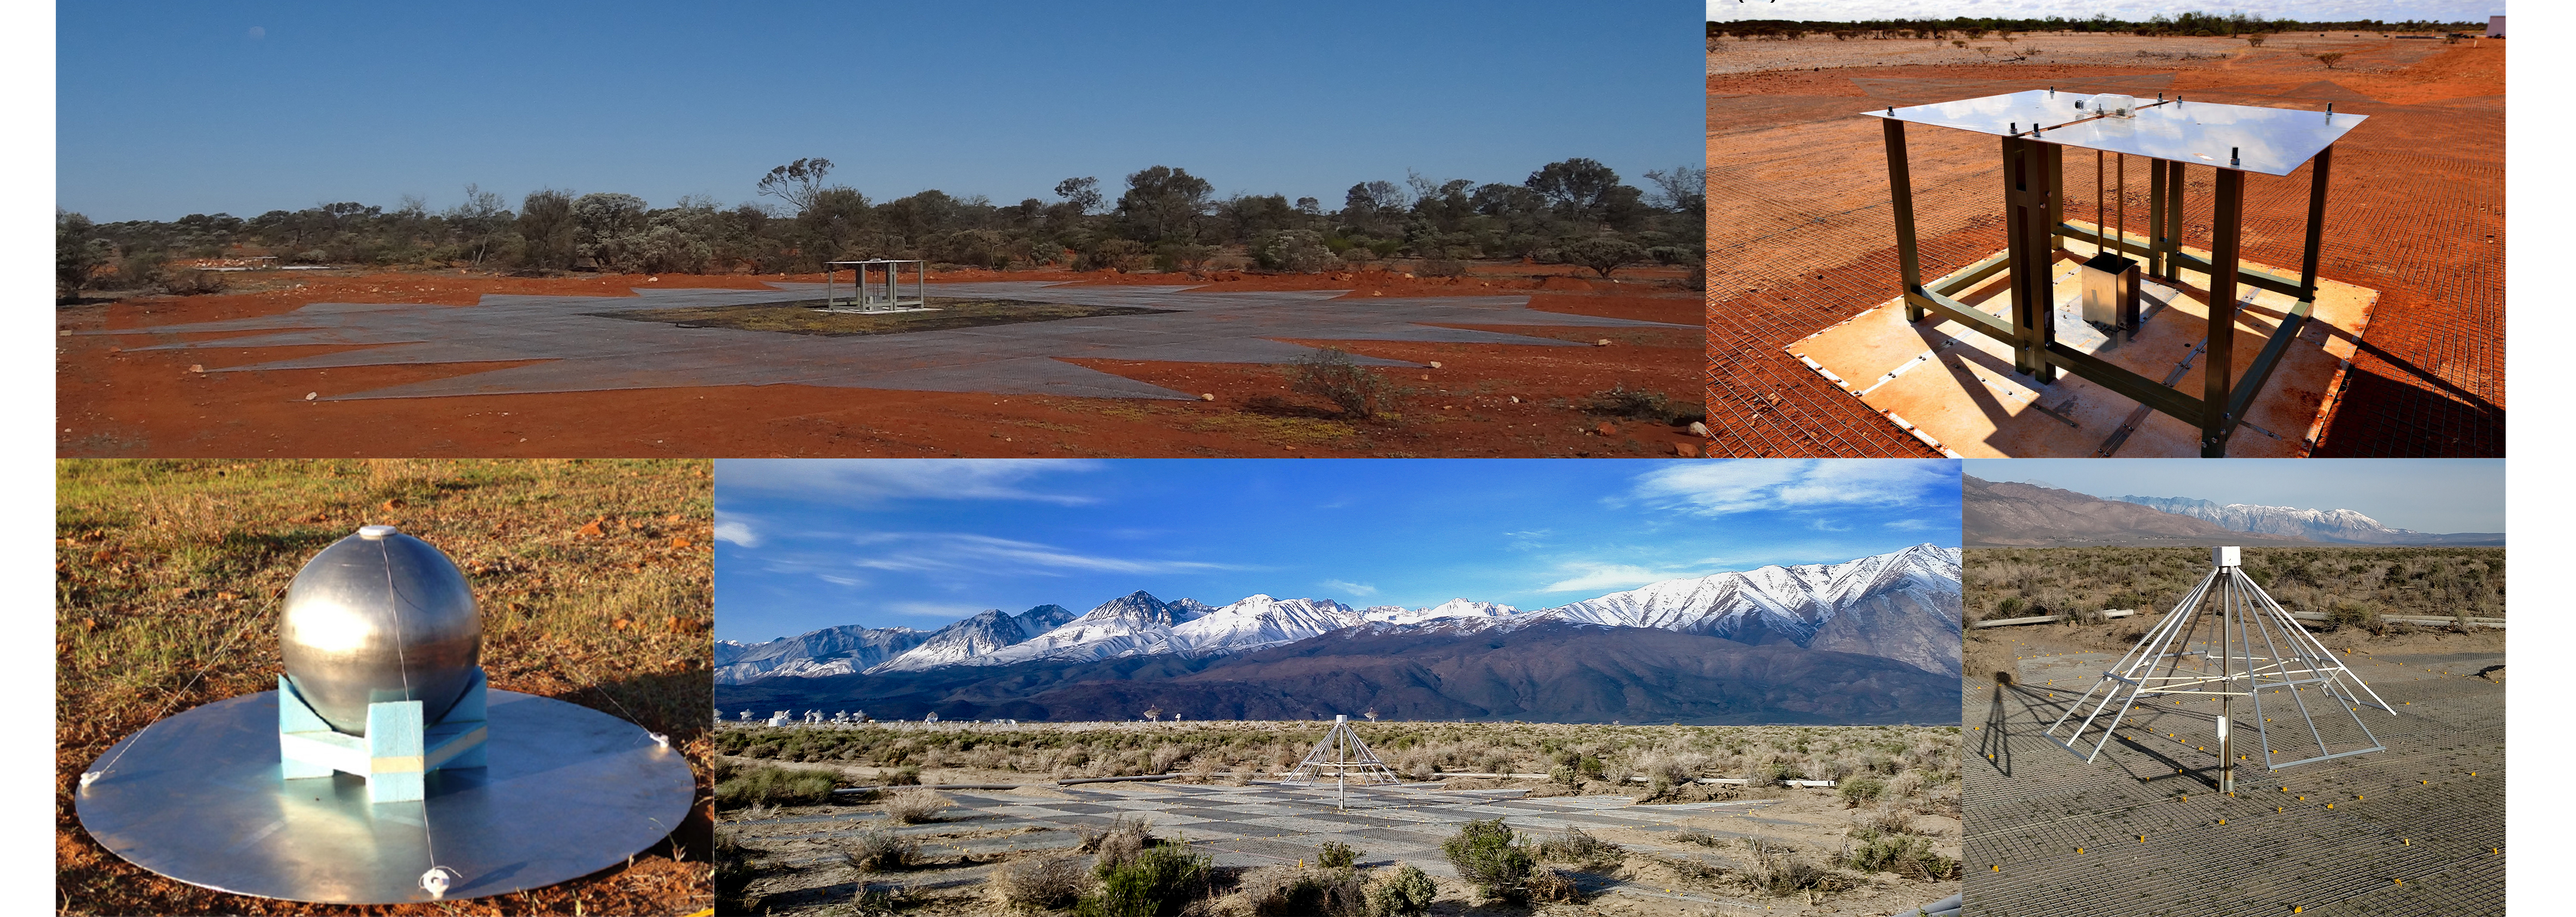
\includegraphics[width=1.05\textwidth]{Greenhill_Subrahmanyan/EDGES_SARAS_LEDA_figure_19sep20.jpg}
\end{center}
\caption{(top left) EDGES antenna and serrated 30~m $\times$ 30~m ground screen.  (top right) Closeup of the EDGES single polarization dipole comprising two rectilinear metal sheets.  (bottom right) Closeup of the LEDA dual polarization pyramidal dipole.  (bottom center) LEDA antenna and serrated 20~m $\times$ 20~m ground screen implemented in 2019. (bottom left) SARAS-2 antenna comprising a spherical element atop a 0.87~m diameter disc.  The maximum gains for EDGES and LEDA antennas are toward zenith.  In contrast, the maximum for SARAS-2 traces a ring on the sky at $30^\circ$ elevation, centered on zenith, where there is a null.}
\end{figure}

\section{Radiometer Basics}

Karl Jansky discovered that any sensor of electromagnetic fields placed beneath open sky samples at its terminals ``cosmic radio noise''\footnote{The term ``noise'' is commonly used because radio frequency (RF) radiation from atomic processes in the cosmos, the ionosphere and troposphere (lightning), and terrestrial thermal sources are spatially and temporally incoherent.  The fields are generally described statistically as Gaussian random variables of zero mean, following from the Central Limit Theorem.}  \cite{jansky33}.  A typical channelized radiometer comprises an antenna, an amplifying receiver that includes a band-limiting filter, a digitizer, and a spectrometer.  The filter defines the measurement bandwidth.   The digitizer samples data at a rate of at least twice the bandwidth.  The spectrometer instantiates Fourier techniques to transform time-series into spectra.\footnote{The theory and implementation of digital spectrometers may be found in \cite{TMS17} and references therein.}  For an Earth-bound antenna, received RF power will include contributions from the cosmos, the ground proximate to the antenna,  self-generated noise from the electronics, and artificial terrestrial interference.  For scale, we note that an antenna with unit gain in equilibrium with a 300\,K blackbody delivers a noise power of {\it O}(1)\,pW over a 100\,MHz band.

\subsection{Antenna}
  
One of the simplest forms of antenna comprises two oppositely directed conductors (a dipole).  Incident waves induce currents in the conductors and a voltage is developed across the inward facing ends (the terminals). The spectrum of power measurable at the terminals corresponds to the incident waves, modified by the frequency-dependent electromagnetic coupling of the antenna and surrounding space (including the ground), antenna efficiency, and transfer function between the terminals and instrumentation downstream.
  
A dipole with wire-like arms each of length one quarter wavelength ($\lambda_0$) will have a sharply peaked resonance and maximum power transfer efficiency at frequency $\nu_0$ in a narrow band $\Delta\nu/\nu_0\ll 1$.  The antenna acts as a transformer from the impedance of free space, $377 \Omega$, on one side to that of transmission lines and RF electronics on the other.  Over a narrow band the impedances of the antenna and RF electronics can be readily matched, and all of the incident power enters the receiver (ignoring resistive losses). 
  
However, the HI signal is inherently broadband, and instrumentation requires at least an octave of bandwidth ($\nu_{\rm high}/\nu_{\rm low}=2$ or $0.66\Bar{\nu}<\nu<1.33\Bar{\nu})$ in order to enable the predicted complex spectral structure due to the 21-cm transition to be distinguished from  smoothly varying foregrounds.  In general, the impedance of a dipole modified to achieve reasonable power transfer efficiency across such broad bandwidths varies considerably in amplitude and phase as a function of frequency.   It can be impossible to match to the RF electronics ``everywhere.''  The consequence is that power is reflected at the antenna-receiver interface and lost. Depending on experiment design, the best that can be achieved with a broadband dipole may be an upper limit on variations in impedance with frequency or an imposed functional form such even in the face of calibration error the variations cannot mimic the science signal.

Broadband dipoles (Figure 1) may be planar with arms comprising 2D shapes (e.g., plates in the case of EDGES), 3D structures comprising planes  (e.g., triangles in the case of LEDA) or more complex structures.  Linear dipoles such as these couple to a single linear polarization mode (with electric field, {\bf E}, oriented along the dipole arms).  Dipoles with spiral and helical arms couple to the circularly polarized mode propagating on axis and jointly to circular and linear modes off axis.  Self-similar planar and conical spirals may have operational bandwidths that exceed an octave and maintain good impedance matching, but other metrics may suffer (e.g., frequency-variable sidelobe structure in gain patterns that generates ``chromaticity'' in antenna response).  Experiments weigh trade-offs differently, typically depending on calibration strategy.

\subsubsection{Ground sensitivity}

Owing to its symmetry, a planar dipole receives radiation incident from the sky and ground equally well.  ``Drooping'' or raising the arms of a linear dipole (e.g., SCI-HI) or projecting a spiral onto a cone--as for the the {\underline B}roadband {\underline I}nstrument for {\underline G}lobal {\underline H}ydrogen {\underline R}eionization {\underline S}ignal--BIGHORNS \cite{sokolowski15}
) are common techniques to break the symmetry, effectively narrowing the field of view and increasing antenna ``directivity.''  However, substantive suppression of coupling to the ground is best achieved by covering it with  a conducting plane.  This ``ground screen'' acts as a reflector.  The antenna senses the sky above {\it and} below, boosting sensitivity for suitable antenna-screen separations (e.g., the direct and reflected paths interfere constructively for $\lambda_0$/4 separation) over some bandwidth. 

Ground screens may be soldered or welded wire mesh, with a minimum conductor spacing or hole size $\ll \lambda_0$, so as to minimize leakage of radiation across the plane.  However, reflection and scattering off the discontinuity represented by the edge of the ground screen creates interference patterns that are functions of the direction and frequency of incident radiation, thereby modulating antenna gain, possibly enough that fluctuations in the received spectrum may be apparent even after calibration.  Adding a random component to the geometry suppresses the effect to a degree.  In telecommunications at high frequencies, fractal-like designs {\it O}($\lambda$) may be etched or milled into a solid metal substrate. However, at low frequencies, sculpting fractals with wire mesh, is impractical.  Instead, implementation of serrated edges has been an effective tool (Figure 1).

%% LJG notes for later.  Confirm adequate treatment of:
%% -Gain pattern characteristics:  achromatic response. 
%% -Electrically small antennas.  Main lobe. 
%% -Antenna impedance characteristics
%% -Tabulation of desirable characeristics that enable radiometry
%%  Editorial comment to consider -- dipoles are good for X.  For 21cm we use them for Y.

% TEXT REMOVED FOR POSSIBLE USE LATER
 %Just as antennas are frequency selective, so also are antenna selective in their direction sensitivity.  I know of no practical antenna that is isotropic.  The relative sensitivity of an antenna across sky directions is referred to as the far-field antenna radiation pattern or beam pattern.  Any antenna is directional and is selective is receiving radiation. A quarter wave dipole antenna is insensitive to radiation incident along its length: after all, radiation incident along that direction would have fields orthogonal to the dipole arms and hence cannot possibly induce currents.  The quarter wave dipole antenna efficiently transduces signals in directions orthogonal to its orientation: quarter wave dipole antennas have toroidal beam patterns; dipole antennas are omni-directional. The larger an antenna is in its electrical size, the more directional is its response to sky radiation.  Antennas with electrical size exceeding unity would naturally have beam patterns that have a main lobe that defines a sky solid angle where sensitivity is maximum, and sidelobes of lower sensitivity.  Electrically small antennas would have a single main lobe without sidelobes.
  
  %Antennas are usually passive systems, hence reciprocal, and may be viewed as radiators or sensors, transforming incident power to signal power at its terminals or transforming power fed at the terminals to free-space radiation.  The antenna as a transformer provides a transformed free-space impedance at its terminals, which is often referred to as antenna impedance. Viewed as a radiator, power fed to the antenna via a transmission line connected to the antenna terminals is only partly available for radiation, because depending on the impedance mis-match between the transmission line and the antenna a part of the power fed to the antenna is reflected back. Of the power available for radiation, a part of the power flows to sky via the main and side lobes of the radiation pattern, a part to ground via what might be considered to be back lobes and a part might be lost as ohmic loss that heats the antenna, if the conducting antenna elements are resistive.  Reflection efficiency of the antenna defines the fractional power available, and radiation efficiency defines what fraction of the available power is radiated into free space.  The antenna views the sky multiplied by the radiation pattern; the weighted average brightness of the sky, with a weighting defined by the radiation pattern, is the sky noise temperature in so far as the antenna is concerned. The radiation efficiency times this temperature is the sky noise temperature component at the antenna terminals, and the reflection efficiency times that terminal noise temperature is the sky noise power propagating down the transmission line.  
  
  %In the context of radiation efficiency, it may also be noted here that if the antenna elements are resistive and there is loss of cosmic signal as ohmic loss in the antenna, not only is there a loss of desired signal but the resistive elements also add their own thermal radio noise to the sky signal. 
  
  %dipole gain patterns are typically broad.  repeating dipoles in parallel giving depth to the structure provide directivity or broad structures, cf. wires  detune but provide coupling over an octave (2x).
 
\subsection{Receiver}

The purpose of an analog receiver is to amplify, over a desired frequency range, the signal coupled to the antenna and passed at it's terminals.  The fluctuating voltage at the terminals propagates along a transmission line to a (typically) modest gain amplifier that boosts signal-to-noise ratios relative to thermal processes in the electronics.  This amplifier too adds noise to the incoming signal, and this is amplified by later stages in the signal path.  There is always a practical trade off between achieving high gain and low noise during amplification, and having the lowest additive noise relative to the sky signal in the first stage amplification is usually paramount, as follows from \cite{friis46}--see also \cite{pozar98} for discussion.  Amplification is most often done in stages, to achieve an aggregate gain sufficient for conversion to a digital signal downstream, without introduction of excessive thermal noise by from particularly high-gain amplifiers. 


\subsubsection{Filtering}

Receivers typically include bandwidth-limiting elements to enhance performance of particular amplifiers or downstream electronics, as for digital processing.  In the former case, filtering is intended to exclude signals that are strong enough to substantively degrade the amplifier linearity, which is susceptible to saturation-like effects, or to create artifacts during amplification where the beating of signals at different frequencies generate products that may be detectable. This is also known as intermodulation (e.g., if broadcast signals above the ``Cosmic Dawn band''  pass through an amplifier, e.g., at 90, 100, and 110 MHz, artifacts may appear in the amplifier output at 10 and 20 MHz).  

For digital processing, filtering serves to suppress the ``aliasing'' of unwanted signals, at frequencies outside the science band, into the band. This occurs when data are sampled at too low rate during digitization.  A digital signal is a sequence of samples.  Sampling with no loss of information requires a rate that is twice the uppermost frequency of interest, as established by the Nyquist-Shannon theorem \cite{TMS17}). Absent application of a sharp low-pass filter corresponding to the top end of the science band, signals at higher frequencies appear to be reflected about the top end and superposed on the science signal.  The unwanted power may be broadcast interference (narrowband) or continuum as from the sky (broadband).

 Common filter topologies are Butterworth, which has a maximally flat, structure-free response, and Chebyshev type 1 and 2, which provides sharper transitions between the passed and rejected intervals but exhibits substantial ripple in one or the other (i.e., the frequency structure to be exiled to where it does the least damage, depending on application).  A third topology, Elliptic, exhibits the same amplitude of structure in the passed and rejected bands, and promises the steepest possible transition from one to the other for a given maximum allowable ripple and magnitude of transition.  Often a combination of filters is used - one to provide excellent rejection but with relatively slower roll-off in response, and others with sharp transitions at the design edges of the passed band.  
   
\subsubsection{Reflection}

Not limited to the antenna-receiver interface, reflection of RF signals occurs at the interfaces between components with different impedances.  A 1\% mismatch in resistive impedance corresponds to a 0.5\% reflection in voltage or 0.003\% in power.  The chain of components along a signal path in a receiver creates instances of multi-path propagation due to numerous fractional reflections.  For well-chosen components, some are negligible, but a complete vector analysis of amplitude and phase is required to understand what frequency structure a receiver may impose in the process of amplifying the input signal.  

In this regard, pairings of filters and amplifiers deserve particular attention.  As noted, filters present frequency structure at their outputs, depending on the selected topology.  They also present frequency structure in reflection at the input. In the case of a low-noise amplifier in the first stage of a receiver, if it is followed by a poorly chosen filter, then it receives back a fraction of its output power but with a potentially complicated frequency-dependent structure imposed.  This propagates upstream through the amplifier (with finite loss, a.k.a. isolation) and reflects off the imperfect antenna-receiver interface and arrives at the amplifier input, added to the cosmic signal and conceivably at detectable levels.

Analysis of multi-path propagation among components applies to additive  thermal noise as well as the amplified sky signal.  Where noise and an attenuated, phase-shifted reflection are co-added during propagation, it develops frequency structure, even though for any given circuit temperature, the noise intrinsically varies slowly and smoothly with frequency.  Because the antenna-receiver interface presents the largest mismatch along the signal path, this is especially important in the case of the first amplifier, from which noise propagates upstream toward the antenna as well as downstream toward later stages of amplification.

A primary engineering formalism describing noise characteristics of linear devices involves a quartet of parameters, one for each frequency:  minimum noise temperature, optimum voltage reflection coefficient (magnitude), the optimum voltage reflection coefficient (phase), and the equivalent noise resistance (referring to the spectral density of noise).  These may be used to estimate the frequency structure impose on noise emanating from amplifiers, as well as the dependence of the amplifier noise temperature on frequency and impedance.  (An amplifier facing a resistive (real) or reactive (imaginary) impedance at its input exhibits different gain and noise temperature.)  Building off \cite{hu04}, \cite{rogers12}  present a simplified formalism for low-frequency systems referred to as ``noise wave'' analysis, which characterizes propagation of noise in terms of correlated and uncorrelated components.  As applied, this works well provided that the reactive component outside the amplifier is sufficiently small. 

\subsection{Digitzer}
  
Analog-to-digital converters (ADC) sample the receiver output at the ``Nyquist rate,'' described above (e.g., 5\,ns for a bandwidth of 100\,MHz).  The number of bits used to represent each sample determines the dynamic range achievable in each spectrum generated by a Fourier transform of every $N$ samples (e.g., for $N=4096$, the frequency resolution, $R$, in the above example is 24.4\,kHz).   The number of bits per sample must be sufficient to represent the range of sky brightness integrated over the antenna gain pattern and prescribed bandwidth. In particular for a sky with a steep spectral index and/or antenna with steep change of gain with frequency, there must be enough bits to represent power at both the highest and lowest frequencies.  At present, transport of an aggregate data rate of {\it O}(2)\,Gbit s$^{-1}$ can be readily achieved, corresponding to 10-bits per sample and a $2^{10}$:1 dynamic range for voltage and $2^{20}$:1 for power.
ADC hardware providing 8 to 16 bits at sample ranges {\it O}(100)\,MHz is readily available.  However, the minimum acceptable bit depth for a given site often depends on the presence and characteristics of interference.  Where peak band-averaged power due to continuous or impulsive interference exceeds that of the sky, representing both without saturation demands greater bit depth in sampling.  Additional considerations arise in  the uniformity of steps during quantization of analog data, linearity over the full analog range, and calibration accuracy where sampling may be parallelized over multiple samplers (a.k.a. interleaving).
 
\section{Challenges Facing Experiments}

\subsection{Antenna Radiation Efficiency}

If an antenna is lossless and has no resistive elements, then when viewed as if it were a transmitting all of the power fed to the antenna, and not reflected back along the transmission line at the antenna terminals, will emerge as radiation.  However, for an antenna placed on bare ground, part of the radiated power may be absorbed.  Low-frequency electromagnetic waves penetrate soil to substantial depths: several meters for dry soil. For antennas that are placed on an infinite conducting ground screen, all of the radiated power goes to sky either directly or on reflection off the ground screen. Passive reciprocal antennas may be viewed conversely as receivers where the loss to resistive elements of the antenna and the loss to the ground both reduce antenna radiation efficiency while adding thermal noise.
   
However, ground loss has a role in mechanisms that create two additional challenges where redress may be more difficult. First, the additive component of ground emission has a complex imprint of the antenna radiation efficiency, making it difficult to separate from zero-mode 21-cm signals unless the antenna is designed so that the radiation efficiency itself has characteristics orthogonal to expectations for zero-mode signals.  Second, the loss depends on ground characteristics, specifically conductivity and dielectric constant, which depend on soil characteristics and moisture content and are functions of depth and time. A sudden change in dielectric constant or conductivity at depth created an impedance discontinuity, as does intrusion of bedrock into the strata.  Such a discontinuity drives multi-path propagation among ground layers and instrumentation above--e.g., see \cite{bradley19}.  Mapping and tracking the RF characteristics of the ground can require extensive additional dedicated instrumentation, such as a network of dielectric impedance reflectometers, and tools to make use of the data are relatively crude at present.
   
Antenna radiation efficiency is also influenced by the environment of the antenna, not only the ground beneath but also feature above, such as shrubs and man-made structures at distances up to several wavelengths.  Conducting cables that supply power to the radiometer and conduct signals to receivers located some distance away may also influence the efficiency.  In measurements of the reflection efficiency as a transmitting antenna, power transmitted by the antenna reflect and scatter off trees and structures in the environment and return to the antenna, as in a radar. Thus measurements of $\Gamma$ sample the environment as well as the antenna.  Conversely, these environmental features will influence the receipt of cosmic radiation in reverse.  Scattering off these objects may generate spectral structure that is an imprint of the environment.  Thus, it is essential to have a clear space above ground and homogeneous if not also dry soil below.

\subsection{Antenna Transfer Efficiency}
   
   The antenna transfer or reflection efficiency, $(1-\Gamma^2)$, which is related to the voltage reflection coefficient $\Gamma$ at the antenna terminals, determines what fraction of cosmic noise received by the antenna propagates into the receiver chain.  In this consideration, it is the impedance of the antenna at its terminals, which is effectively the free space impedance transformed by the antenna to its terminals, as compared to the impedance of the first low noise amplifier encountered by the cosmic noise as transformed by the interconnecting transmission line to the antenna terminals, that decides the reflection coefficient $\Gamma$.  
   
   A design goal for zero-mode 21 cm is an antenna that has high reflection efficiency over the full observing band.  However, since the foreground Galactic sky has a brightness temperature that is significantly greater than the noise temperatures of modern low noise amplifiers operating in the 10-200 MHz band, it is sufficient that the total efficiency of the antenna provide an antenna temperature that well exceeds the receiver noise.  In that case, the system temperature and hence the measurement noise for any integration time would be independent of the receiver noise and improving the total efficiency would not improve detection sensitivity or reduce the required observing time.
   
   What is probably of greater importance is that the reflection efficiency be a smooth function of low order so that the product of the relatively bright foreground sky with the reflection efficiency, to give the dominant unwanted component of the observed spectrum, does not confuse the desired zero-mode 21 cm signal, and is separable from the 21-cm signal.  If the antenna structure is electrically long, as would be the case, for example, in frequency independent spiral antennas with large structural bandwidth, the reflection efficiency would have fine structure in frequency.  Therefore, from the viewpoint of designing the antenna element to have reflection efficiency that is exclusively of low order, it is advantageous to have electrically small antennas.
   
   If the antenna does not have resistive elements, and the radiation efficiency is unity, then a measurement of the antenna reflection efficiency $\Gamma$ would be a useful method for correcting the data for antenna efficiency and translating the measured spectrum to a sky spectrum. In this case, it is desirable and useful to provide a switch at the antenna terminals, which might allow a 1-port network analyser to access the antenna terminals and make an accurate measurement of $\Gamma$.  This is best done at the observing site, where the antenna environment is the same as for the zero-mode observing.  Deriving the reflection efficiency and total efficiency requires also a measurement of $\Gamma$ for the low-noise amplifier, but that may be done in the laboratory provided that the amplifier temperature and operating conditions are the same.

\subsection{Gain Pattern}

A critical challenge in antenna design is suppression of ``mode coupling.'' This arises when an antenna gain pattern is chromatic, i.e., for each direction, gain varies with frequency. \footnote{We note in passing that there is no general, compact, quantitative definition of chromaticity.}   Even for a sky with a constant spectral index, the consequence of chromatic response is potentially complex frequency structure everywhere on the sky.  

Mode-coupling can be a fundamental hurdle to detection of the 21-cm signal with any given antenna.  The most certain means to suppress it is to adopt antennas that are achromatic, i.e., frequency-independent in gain in all directions.  Chromaticity may not be easily quantified, but spectra being limited by statistical noise rather than undulations in the spectral baseline can be an effective figure of merit.  Servicing this, spectra simulated using calculated gain patterns and sky models may be used in tuning antenna designs to achieve a required level of a-chromaticity.

\subsubsection{Measurement and Simulation}

High-accuracy direct calibration of gain patterns {\it in situ} (thereby taking into account all details of coupling to the ground, structures, ground screens, etc) is an unsolved problem.  There are no suitable standard antennas in communications engineering.  Lofting transmitters on drones has been developed \cite{jacobs17}, but cancellation of systemtics intrinsic to this scheme (e.g., multi-path and uncertainty in the gain pattern of the transmitting antenna) has not been demonstrated and confirmed.  The most widely employed alternative is numerical simulation.

Arguably, most available electromagnetic simulation packages are not capable of providing solutions with the precision necessary to quantify antenna response, though cross-referencing of results enables assessment of systematics stemming from the various simulation techniques applied.  Exacerbating the above difficulty is the need to include in simulations coupling to stocastic elements in the surroundings (vegetation), soil chemistry, and time-variable changes in water content. Antennas also couple to strata below ground with complex permittivities (i.e., non-zero conductivity) and infrasructure such as trenched cables.  In general the design path necessarily requires iteration to achieve exacting performance tolerances, and cross-referencing results obtained with different packages.   

\subsection{Cosmic Foregrounds}

At millimeter wavelengths where the CMB peaks the sky is dominated by the CMB. Galactic emission and the extragalactic background are sub-dominant.  At frequencies relevant to the 21-cm transition at high $z$, the radio sky is qualitatively different, dominated by synchrotron emission from the Galactic plane, which extends to considerable latitudes, and diffuse off-plane components.  As well, in neither case is the structure readily modeled in angle or frequency, not least because position-resolved spectra of the sky at these low frequencies are known with accuracies of only {\it O}(10\%).  Moreover, there are no known fiducial tracers that may be used to establish external constraints.

The peak amplitude of the cosmic 21-cm signal is expected to be a few tens to a few hundred mK, and the foreground is expected to between a few hundred to a few thousand Kelvin brightness temperature.  This requires a dynamic range of at least $10^4$, clean signal detection requires aiming for dynamic range of $10^5$.  Because the algorithms for components separation, which depend on orthogonality between the zero-mode 21-cm signal and other unwanted additives and foreground, are usually limited and the models for the unwanted components would subsume a significant part of the 21-cm signal; therefore, the typical design goal for the 21-cm radiometers is to achieve an artifact-free spectrum of {\it O}(1)\,mK sensitivity, about $10^6$ below the dominant foreground.

\subsection{Ionosphere}

The ionosphere has time varying electron densities that is commonly characterized by the total electron content (TEC) along any line of sight.  The ionosphere modifies spectra of background sources in several ways.  It refracts rays, so that sources appear at higher elevations \cite{vedantham14}.  The ionosphere also both absorbs the background and adds emission from populations of hot electrons \cite{rogers15}. These effects of the ionosphere are strongly wavelength dependent and are anticipated to predominantly modify radiation at $\nu\lesssim 100$\,MHz.

In general, the accuracy and spacing of TEC measurements is as yet inadequate to support time-varying correction of measured sky spectra.  TEC data are primarily of use in deciding the relative severity of ionospheric conditions and the order of magnitude of distortions to be anticipated in spectra--a coarse weather report.  Consequently, analyses of radiometry data  must include model nuisance parameters that describe ionosphere effects, requiring marginalization in order to extract the zero-mode signal from data.  

\subsection{Polarization}

Galactic and extragalactic foregrounds comprise sources often with significant fractional  linear polarization.  The detected foreground spectrum will be polarisation dependent.  Complications arise due to Faraday rotation of differing degrees.  The effect is frequency  dependent, and for a linearly polarized source, the source intensity received by any single polarization will be frequency dependent.  Hence, Faraday rotation results in spectral structure that may potentially confuse attempts to detect zero-mode 21-cm spectral structure. For this reason, it is desirable and a design goal for zero-mode radiometers to be dual polarised pair of radiometers, with full polarisation calibration that allows derivation of the Stokes I component on the sky.


\subsection{Interference}

Virtually all frequencies at which a zero-mode signal corresponding to the EOR or CD could appear are allocated to terrestrial and space communications. Transmitters at these frequencies exist in most parts of the world, and propagation paths may be line of sight, reflected (e.g., off meteor trails and aircraft), or bent by diffraction around obstacles. Extremely remote sites exist where interference due to long-range propagation is rare \cite{voytek14,philip19}, but apart from these unusual cases, low-frequency radiometry data is corrupted intermittently, raising the possibility of weak interference contributing weak artifacts in spectra.  These may be narrow band (e.g., FM transmission) or broadband (e.g., digital television, where each channel allocation is several MHz wide).  They may be recognizable as discrete spectral features or solely by deviations from Gaussian statistics in time-series.


\section{Pr\'ecis of Design Requirements}


\begin{itemize}
    \item[1.]
    {\bf Radiometer bandwidth}: an octave or more, to enable separation of smooth-spectrum foregrounds and the distinctly not smooth 21-cm spectral signature.
    
    \item[2.]
    {\bf Antenna gain pattern {\it in situ}}: maximally smooth in angle and frequency with minimum chromaticity, and characterization from direct measurement or simulation if necessary.
    
    \item[3.]
    {\bf Ground screen}: large enough to isolate the radiometer from propagation in ground strata and buried infrastructure); sufficient geometric irregularity along the edges so as to suppress coherent patterns in scattering of incident radiation toward the antenna. 
    
    \item[4.]
    {\bf Antenna polarization}: dual polarization to enable construction of Stokes I and cancel artifacts that can arise from Faraday rotation of foreground emission.
    
    \item[5.]
    {\bf Site}:  a radiometry site with a clear horizon out to several wavelengths, and related to item no. 3,k homogeneous dry strata below.

\end{itemize}



   
   
%\subsection{Reflections within the Signal Path}

 % Impedance discontinuities in the receiver path cause internal reflections of the system noise, which includes the cosmic noise component and also the receiver noise.  Reflections of wideband noise over a physical length $l$ result in interference that cause spectral structure with frequency scale $v/2l$, where v is the propagation speed of electromagnetic waves in the physical medium.  For example, internal reflection within a cable of length 2 metres between the antenna and low-noise amplifier, with velocity factor 0.7, will result in spectral ripples with period 52.5 MHz. These structures would be a modulation of the receiver gain, and hence calibrated out, if the calibration includes these sections in their entirety.  However, if the receiver calibration is internal, then reflections from the antenna terminal and also reflections of receiver noise from environment are omitted from the calibration.  Ideally, receiver gain calibration using celestial sources, such as the passage of the Galactic plane across the radiometer beam, would best calibrate the signal path.  In any case, it is desirable that the signal path have isolators that prevent back flow of signal path components to the antenna.  Improved isolation also comes from use of amplifiers in which the forward gain is substantially greater than the reverse isolation, so that the net loss on propagation back and forth is substantial.
  
  
%\subsection{Analog to digital conversion}
 
% A key component in the signal processing in a zero-mode 21-cm radiometer is the conversion from continuous to discrete data.  Random and systematic errors in the representation of the analog signal leads to performance limitations.  An important design consideration is the number of bits in the analog to digital converter.  Larger effective number of bits is essential for greater spurious free dynamic range.  A design goal of $10^6$ for dynamic range requires 10 effective bits, which implies analog to digital converters of 12 bits or greater.  The quality in the transfer function of the converter is also required to be accurate so that the spurious free dynamic range is $10^6$.
 
%\subsection{Radio Frequency Interference (RFI)}
  
%  Radio frequency interference (RFI), if present at the observing site, would naturally require improved performance of the radiometer to avoid spurious spectral structure that might confuse the zero-mode signal.  In good sites, it is expected that the total power in RFI would be well below the total band power from cosmic noise.  This is facilitated by adopting small antenna designs that have low gain, low effective collecting area, so that the cosmic noise is received without compromise but response to RFI is reduced. 
 
% Presence of radio frequency interference may drive the design to lower the power in the cosmic noise going to the analog to digital converter, so that the signal is not clipped in the sampling, which would lead to non-linear products spread across the band.  Lowering the power in the cosmic noise, to provide greater headroom for the RFI components when they might occur, reduces the effective number of bits operating on the cosmic noise, thus requiring greater performance of the analog to digital converter.
   

%\subsection{Receiver Design}

%The receiver modifies the cosmic radio spectrum in its bandpass, and adds receiver noise; these require bandpass calibration and correction of the measurement data for additives.  Most receiver designs adopt methods for cancellation of additives, via switching schemes.  However, there may be additives that suffer multi-path propagation that includes reflection off the antenna impedance, which may not be canceled.  In such cases, receiver designs often incorporate isolators and also minimise physical lengths of multi-path propagation, so that the unsubtracted additives are restricted to be of low order and hence largely orthogonal to the 21-cm signals.


\section{Outside the Box Architectures}

\subsection{Single-element Sensor  Radiometer}
  
  The simplest form of a radio telescope that would be appropriate for detecting the zero-mode 21-cm signal is a single elemental wideband antenna followed by a spectrometer.  Such a radiometer would ideally have a frequency-independent antenna, a self-calibratable receiver that corrects for the bandpass, and switching schemes to cancel internal additives including receiver noise.
  
  The considerations that drive the design of such a radiometer have been discussed above.  Limitations and design challenges to the performance of such a single-element spectral radiometer are manifold.  Therefore, there have been new concepts and design attempts to develop alternate schemes or configurations that might avoid some of the potential show stoppers.
  
\subsection{Outriggers to Fourier Synthesis Telescopes}
  
  A key challenge in zero-mode 21-cm radiometers is knowing the antenna beam pattern, its chromaticity, and the bandpass of the antenna element.  Antenna measurements at long wavelengths are exceedingly difficult because of the parasitic effects of environment and the ground, which influence both the device under test and also the test and measurement antenna.  Switched calibration, using broad band noise sources, may serve to calibrate the bandpass of the receiver chain; however, this leave the antenna bandpass, radiation efficiency, uncalibrated.  This leads to a situation where the antenna characteristics may have to be derived from electromagnetic simulations, which may not have the accuracy needed for correction of the measurement data.
  
  A solution to these issues is to deploy the single-element sensor based radiometer as an outrigger to an array of antennas, which operate in Fourier synthesis interferometer mode.  The radiometer antenna and receiver chain then form another element of the array, which together observe the sky sources within the antenna primary beams.  The measured spectral visibilities are then used to solve simultaneously for the sky model and also the instrument parameters, which include the bandpass and beam shape of the outrigger antenna. If all array elements are dual polarised, then full Stokes calibration is also possible, providing polarisation calibration solutions as well for the outrigger antenna.
  
\subsection{Interferometric Methods}
  
  It is not often appreciated that interferometers are not totally blind to the zero-mode in the sky temperature distribution.  If the sky were uniformly bright, then the electromagnetic fields at two points in space separated by less than a wavelength will show mutual coherence, which may be measured by an interferometer.  A pair of half-wave dipoles placed adjacent to each other, in line, will respond to the zero-mode of the sky temperature distribution.  If placed parallel to each other the interferometer response will contain the zero mode, and the response in this case will be greater.  The interferometers may be thought of as sampling the zero-mode in the direction in which the projected spacing between the elements in zero.  Of course, if the spacing between the dipoles increases, the response falls off progressively.
  
  The coupling of the interferometer response to the zero-mode signal depends on the mutual coupling between the aperture fields in the pair of antennas.  This is relatively high for closely spaced elemental antennas; however, a pair of aperture antennas placed adjacent to each other would have very little response to the zero-mode if their aperture illuminations have little overlap.
  
  Interferometers have the advantage that when they deploy a pair of sensors of the electromagnetic field at two separated locations in space, and measure the mutual coherence in the fields by cross correlating the received and amplified voltage waveforms, they are insensitive to the additive receiver noise in the two arms, which are uncorrelated.  
  
  Thus interferometer measurements are blind to internal receiver additives, thus scoring over single element radiometers on this count.
  
\subsection{Zero-spacing Interferometer}
  
  If a pair of wideband antennas are placed adjacent to each other, with mutual coupling between the antennas, then the interferometer response includes the zero-mode signal.  This response may be enhanced by placing a vertical beam splitter in between the antennas, so that incident field from any side propagates to the antenna on the far side through the screen and to the near side in a direct path and also after reflection off the screen.  If the beam splitter is reactive, and lossless, then the response to zero-mode on the two sides of the screen cancel.  However, if the beam splitter is resistive, then the interferometer responses add with the same sign.  Optimally, it can be shown that the sensitivity is a maximum if the beam splitter has a sheet resistance equal to the impedance of free space.  
  
  Interferometers made from elemental antennas placed in a close packed configuration will have a telescope filter function, which defines the interferometer response to zero-mode 21-cm signals, that is highly frequency dependent and challenging to calibrate.  The advantage of the zero-spacing interferometer made from frequency independent antennas is that the telescope filter function in this case is flat, at least over the frequency range in which the resistive screen is frequency independent.  
  

\subsection{Lunar Occultation}
  
  An alternate and interesting approach to detection of the zero-mode 21-cm signal is via Fourier synthesis imaging of the Moon.  The brightness measured towards the Moon, over frequency, would be a difference between the Moon brightness and the mean brightness of the radio sky.  Thus if the Moon were assumed to be of flat spectrum, or if the temperature spectrum of the Moon were known, then the differential measurement may be used to infer the zero-mode 21-cm signal.
  
  The measurement is not without difficulties.  Firstly, it is not clear that the temperature spectrum of the Moon is flat of even smooth; the lunar regolith may have structure and layered in depth, which would give spectral structure in the emission brightness.  Additionally, the Moon is reflective and hence the brightness of the Moon has a component that is a reflection of the radio sky. Finally, the synthetic beam of the Fourier synthesis telescope will have sidelobes that are chromatic; thus mode coupling will induce spectral structure whose removal from the data will be limited by the depth of deconvolution. 
    





%=============================================

\bibliographystyle{plain}
\bibliography{Greenhill_Subrahmanyan/References}
%\bibliography{./references}

%=============================================




\chapter{Status of 21~cm interferometric experiments}

\begin{bf}
  \author{Cathryn M. Trott (ICRAR-Curtin), Jonathan Pober (Brown University)}\\
  
Abstract\\
\end{bf}

This chapter discusses the history, progress, challenges and forecasts for detection and exploration of the spatial structure of the 21~cm brightness temperature signal in the Epoch of Reionisation using interferometric experiments. We discuss GMRT, PAPER, LOFAR, MWA, LEDA, and the future HERA and SKA.


\section{High-level topics}

\begin{itemize}
\item Historical perspective - CMB studies, early arrays
\item Current and recent experiments - description of instruments and experimental design; fundamental differences in analysis and observation methodologies and choices made. LOFAR, MWA, PAPER, GMRT, LEDA (MITEoR?)
\item Exploration of published results; retractions; upper limits; foreground techniques
\item Current challenges: signal loss, leverage, calibration coupling, incomplete sky models and instrument models. How do we know we have detected something?
\item Future prospects for current instruments
\item Future instruments; design, experiments. HERA, SKA. Potential for success. Cross-correlation studies to help with robust signal detection
\end{itemize}



\begin{figure}[]
\begin{center}
\includegraphics[width=0.5\textwidth]{Trott_Pober/01x01-eps-converted-to}
\end{center}
\caption{This is figure 1 in chapter 1.}
\end{figure}

\paragraph{Cras adipiscing} sagittis nunc vel luctus. Suspendisse volutpat augue quis erat semper consequat dignissim tellus euismod. Morbi hendrerit, tellus id aliquam iaculis, nibh leo tincidunt eros, vitae varius ligula felis in mi.

\begin{table}
\caption{Greek Letters.}
\begin{center}
\begin{tabular}{llllllll}
\hline
$\alpha $  & $ \beta $  & $ \gamma $  & $ \delta $  & $ \epsilon $  & $ \varepsilon $  & $ \zeta $  & $ \eta $ \\
 $ \theta $  &  $ \vartheta $  &  $ \gamma $  &  $ \kappa $  &  $ \lambda $  &  $ \mu $  &  $ \nu $  &  $ \xi $ \\
 $ o $  &  $ \pi $  &  $ \varpi $  &  $ \rho $  &  $ \varrho $  &  $ \sigma $  &  $ \varsigma $  &  $$ \\
 $ \tau $  &  $ \upsilon $  &  $ \phi$ &  $ \varphi $  &  $ \chi $  &  $ \psi $  &  $ \omega$  &  $ $ \\
 &  &  &  &  &  &  & \\
$ \Gamma $  & $ \Delta $  & $ \Theta $  &  $ \Lambda $  &  $ \Xi $  &  $ \Pi $  &  $ \Sigma $  & $ \Upsilon $ \\
 $ \Phi$ &  $ \Psi $  &  $ \Omega $  &  &  &  &  &\\
\hline
\end{tabular}
\end{center}\end{table}

\begin{figure}[]
\begin{center}

\includegraphics[width=0.6\textwidth]{Trott_Pober/01x02}
\end{center}
\caption{This is figure 2 in chapter 1.}
\end{figure}


\bibliographystyle{plain}
\bibliography{Trott_Pober/References}



\chapter{Future prospects}
\label{chapter:koopmans_bernardi}

\begin{bf}
  \author{Leon V. E. Koopmans (Kapteyn Astronomical Institute), Gianni Bernardi (INAF-IRA \& Rhodes University)}\\
  
Abstract\\
\end{bf}

This chapter discusses some important things




\section{Forthcoming interferometric ground based instruments and upgrades}

In this section we review the status of the 21~cm ground based interferometers that are under construction, have been upgraded or will be constructed in the near future.

\subsection{The Hydrogen Epoch of Reionization Array}
\begin{figure}[]
\begin{center}
\includegraphics[width=1.\textwidth]{Koopmans_Bernardi/hera_layout}
\end{center}
\caption{The HERA layout (left panel): 320~dishes are located in the hexagonal core and 30 more outrigger dishes are planned to be deployed out to a maximum baselines of $\sim 800$~m to improve angular resolution and imaging capabilities. The core is split in three sectors that are displaced from each other by a fraction of the dish diameter (see \cite{dillon16} for a detailed discussion. The split core provides a significantly improved instantaneous $uv$ coverage (central panel) whilst retaining high redundancy. The right panel shows the expected relative antenna gain errors after using redundant calibration (from \cite{dillon16}).}
\label{fig:fig_hera}
\end{figure}
The Hydrogen Epoch of Reionization Array (HERA, \cite{deboer17}) is an array currently under construction in the Karoo reserve area in South Africa - following the decommissioning of the PAPER experiment (see Chapters~\ref{chapter:bernardi} and 8 in this book for an overview of PAPER). HERA is built following the approach used for PAPER: a highly redundant array to maximize the sensitivity on a number of power spectrum modes measured using the avoidance approach. In order to increase the sensitivity with respect to PAPER, it employs 14~m diameter non steerable dishes that, in the final configuration, will be densely packed in a highly redundant hexagonal array configuration of $\sim 350$~m diameter (see Figure~\ref{fig:fig_hera}). 
HERA main goal is to measure the 21~cm power spectrum in the $6 < z < 12 $ range with high significance in the $0.2 < k < 0.4$~Mpc$^{-1}$ range (\cite{pober14}, providing a full characterization of the evolution of the neutral Hydrogen fraction of the intergalactic medium (Figure~\ref{fig:fig_hera_ion_hist}).
\begin{figure}[]
\begin{center}
\includegraphics[width=1.\textwidth]{Koopmans_Bernardi/hera_ion_hist}
\end{center}
\caption{95\% confidence region on the Hydrogen neutral fraction $X_{\rm HI}$ (grey, from \cite{greig17}). The inclusion of HERA measurements leads to a dramatic improvement in the constraints (red and pink areas, \cite{liu16b}). Constraints from other reionization probes are shown as well (see \cite{deboer17} for a detailed description).}
\label{fig:fig_hera_ion_hist}
\end{figure}

Given the high redundant configuration, imaging tomography will remain challenging for HERA and likely the goal of a future generation experiment. As foreground modeling and characterization will also be limited because of redundancy and the coarse angular resolution, a significant effort was dedicated to keep the instrumental response from corrupting the intrinsically smooth foreground spectra and to accurately model it (\cite{neben16}, \cite{ewallwice16}, \cite{thyagarajan16}, \cite{patra18}). An alternative approach to redundant calibration is to apply foreground avoidance using closure phase quantities from antenna triads (\cite{thyagarajan18}): closure phase are insensitive to errors in direction independent interferometric calibration and, therefore, directly bypass the requirement of an accurate spectral calibration (see Chapter~\ref{chapter:bernardi} in this book for an overview of calibration of 21~cm observations). A preliminary analysis of HERA closure phases seem to confirm these premises (\cite{carilli18}).

HERA is currently under construction, with more than 200 dishes deployed, and 21~cm observations are currently being analyzed. New feeds that extend the sensitivity to the 50-250~MHz range are currently deployed for testing in order to enable observations in the $12 < z < 35$ range (the Cosmic Dawn) and probe the nature of the first luminous sources and their impact on the thermal history of the intergalacic medium.



\subsection{The Large aperture Experiment to detect the Dark Ages}
\label{section:leda_pspec}
\begin{figure}[]
\begin{center}
\includegraphics[width=1.\textwidth]{Koopmans_Bernardi/lwa_layout}
\end{center}
\caption{LEDA antenna layout: the dense core is surrounded by 32 dipoles in order to provide an exceptionally good instantaneous $uv$ coverage (from \cite{eastwood18}).}
\label{fig:fig_leda}
\end{figure}
The Large aperture Experiment to detect the Dark Ages (LEDA, \cite{bernardi15}, \cite{kocz15}) is located at the Owens Valley Radio Observatory, California. It operates in the 30-88~MHz frequency range, corresponding to $15 < z < 46$, seeking to detect the 21~cm signal from the Cosmic Dawn.   
The array layout consists of 251 dipoles pseudo randomly deployed within a 200~m diameter core, 23 dipoles are added out to a maximum 1.5~km baseline (see Figure~\ref{fig:fig_leda}). Five additional outrigger dipoles are custom-equipped to measure the global 21~cm signal via individual custom-built dipoles (see Section~\ref{leda_global}).

The very dense core provides exceptional brightness sensitivity and a point spread function with very low sidelobes. The outrigger dipoles improve the angular resolution that helps to identify calibration sources and lower the confusion level. As the dipoles are individually correlated, visibilities have contributions from all-sky emission, particularly from Galactic diffuse emission - given the number of short baselines - and with significant ionospheric-induced refraction and scintillation. Despite these challenges, \cite{eastwood18} generated the first high quality all-sky foreground maps. 

The LEDA approach to measure the 21~cm signal can be versatile, allowing to image and subtract foregrounds (\cite{eastwood18}) but also to avoid them (similar to \cite{beardsley16}). \cite{eastwood19} analyzed 20~hours of LEDA data calibrated using a compact source sky model and filtering foregrounds by using their statistical properties in way similar to \cite{dillon14} and \cite{trott16}. They reported an initial $10^8$~mK$^2$ upper limit on the 21~cm power spectrum at $z = 18.4$. Several hundreds of hours of observations have been collected now and will be the focus of future analysis towards the detection of the power spectrum from the Cosmic Dawn and an independent confirmation of the reported detection by \cite{bowman18}.



\subsection{The Low Frequency Array}
\label{section:lofar}



\subsection{The Murchison Widefield Array phase II}

Chapters~\ref{chapter:bernardi} and 8 have already described the relevant aspects of the MWA phase II upgrade. Here we emphasize the improved sensitivity to the 21~cm power spectrum due to the addition of the two redundant hexagon near to the core. Figure~\ref{fig:fig_mwa_phaseII_pspec} shows a sensitivity improvement of a factor of four with respect to the phase I and $\sim 10\sigma$ detection of the fiducial 21~cm power spectrum at $k \sim 0.1$~Mpc$^{-1}$. {\bf (GB: Leon, are you ok with this summary?)}
\begin{figure}[]
\begin{center}
\includegraphics[width=1.\textwidth]{Koopmans_Bernardi/mwa_phaseII_pspec}
\end{center}
\caption{Fiducial 21~cm power spectrum model at $z = 8.5$ with associated noise levels from Phase I and Phase II arrays with a 1000~hour observation. ``Phase II 256" shows the result from a future MWA upgrade where all 256 tiles are correlated simultaneously (from \cite{wayth18}).}
\label{fig:fig_mwa_phaseII_pspec}
\end{figure}




\section{Forthcoming Global Signal Experiments}

In this Section we review the status of the ongoing global signal experiments (see Chapter~7 for a more detailed discussion about global signal observations).

\subsection{The Experiment to Detect the Global EoR Signature}
%\begin{figure}[]
%\begin{center}
%\includegraphics[width=1.\textwidth]{Koopmans_Bernardi/edges_trough}
%\end{center}
%\caption{EDGES}
%\label{fig:fig_edges}
%\end{figure}
The Experiment to Detect the Global EoR Signature (EDGES, \cite{bowman08} currently operates in two frequency bands: the $90-200$~MHz band (high band) in order to constrain the evolution of the neutral fraction throughout reionization, and the $50-100$~MHz band (low band), in order to measure the expected heating of the intergalactic medium from the primordial sources. 
The EDGES experiment has been pioneering techniques to accurately model all the various instrumental components in order to carefully control systematics effects. Observations in the high band have constrained the duration of reionization $\Delta z$ to be longer than $\Delta z >  1$ and started to constrain some properties of the first galaxies (\cite{monsalve17}, \cite{monsalve18}). In the low band, \cite{bowman18} reported the surprising detection of an absorption trough twice as deeper than the most extreme models, posing a serious challenge to its interpretation - assuming it is of cosmological issue. 

In the light of this anomalous signal, the EDGES team is deploying a new dipole antenna tuned in size to simultaneously observe the $60-160$~MHz range (i.e. $\sim 25\%$ smaller than the low band antenna) and confirm the results in the low band. A further upgrade of the EDGES experiment with a more portable antenna that includes the electronics is under consideration for deployment in a quiet radio frequency environment in Oregon, USA.



\subsection{The Large aperture Experiment to detect the Dark Ages: status and perspectives of global signal measurements}
\label{leda_global}
%\begin{figure}[]
%\begin{center}
%\includegraphics[width=1.\textwidth]{Koopmans_Bernardi/leda_dipole}
%\end{center}
%\caption{LEDA dipole}
%\label{fig:fig_leda_dipole}
%\end{figure}
As mentioned in Section~\ref{section:leda_pspec}, LEDA includes a few custom-equipped dipoles to measure the global signal (\cite{price18}, see also Chapter~7 in this book). Initial observations were used to validate the end-to-end acquisition system and data analysis, leading to a 890~mK upper limit on the global signal amplitude in the $13.2 < z < 27.4$ range at the 95\% confidence level (\cite{bernardi16}). A series of upgrades have been implemented since the early system: filters with a sharper roll-off were installed in order to improve RFI rejection and extend the observing band up to 87.5~MHz in order to validate the results by \cite{bowman18}; the stability of the noise diodes has been improved and a system to measure the ambient temperature at the antenna has been installed. The receiver seems to show the necessary stability to measure the global signal, however, other sources of systematics related to the antenna gain pattern remain lees well known and are the subject of ongoing modeling and investigation.

About 100~hours of observations were taken with the upgraded system and are currently being analyzed.

{\bf (GB: this section may be removed if already included in Chapter~7, I cannot see that chapter yet...)}


\section{Current and planned space based instruments}

\subsection{The Dark Ages Polarimetry Pathfinder}
The Dark Ages Polarimetry Pathfinder (DAPPER, \cite{burns19}) is a space satellite that is intended to observe the global signal from a $50 \times 125$~km lunar orbit, one of the quietest radio frequency environments, with an expected 26~month liftime. Its goal is to observe the global signal absorption trough that is expected at $35 < z < 80$, well before the formation of the first luminous sources (see Chapter~2 in this book). In this epoch, the global signal profile is purely determined by cosmology in the linear regime without being affected by complex astrophysical processes. DAPPER is expected to characterize the expected global signal, including any deviation that may be due by the additional cooling reported by \cite{bowman18}. Its strategy includes the use of a polarimeter to measure polarization induced by the anisotropic foregrounds and large antenna beam to aid in the separation of the foregrounds from the isotropic, unpolarized global signal (\cite{nhan17}) and a pattern recognition data analysis that is trained on realisti smulations of observed foregrounds, instrument systematics and the expected global signal (\cite{tauscher18}).

DAPPER is one of nine smal satellite missions selected by NASA to be further study for a possible launch in the next decade.

%We report on the results of a NASA-funded Astrophysics SmallSat concept study for a proposed lunar-orbiting experiment, the Dark Ages Polarimeter PathfindER (DAPPER), that is designed to observe the unexplored Dark Ages epoch of the early Universe. The Dark Ages, probed by the highly redshifted 21-cm neutral hydrogen global signal, is the ideal epoch for a new rigorous test of the standard LCDM cosmological model. DAPPER will search for divergences from the standard model that will indicate new physics such as heating or cooling produced by dark matter. A broad absorption trough in the redshifted 21-cm spectrum is expected during the Dark Ages, prior to the formation of the first stars and thus determined entirely by cosmological phenomena. DAPPER will observe this pristine epoch (17-38 MHz; z 83-36), and will measure the amplitude of the 21-cm spectrum to the level required to distinguish (at >5-\u03c3) the standard cosmological model from that of additional cooling derived from recent EDGES results. The main challenge of this measurement is the removal of bright foregrounds. DAPPER is designed to overcome this by utilizing two pioneering techniques: (1) a polarimeter to measure polarization induced by the anisotropic foregrounds and large antenna beam to aid in the separation of the foregrounds from the isotropic, unpolarized global signal, and (2) a pattern recognition analysis pipeline based on well-characterized training sets of foregrounds from sky observations, instrument systematics from simulations and laboratory measurements, and signals from theoretical predictions. End-to-end simulations of the DAPPER instrument including thermal noise, systematics from the spectrometer/polarimeter and the beam-averaged foreground, along with 21-cm models which include added cooling meet our sensitivity requirements to separate the standard cosmological models from ones that point toward new physics. DAPPER's science instrument consists of dual orthogonal dipole antennas and a tone-injection receiver based on high TRL components from the Parker Solar Probe/FIELDS, CURIE, and WIND/WAVES. DAPPER will be deployed into a frozen 50x125 km lunar orbit to provide 4615 hours of radio-quiet integration over a 26 month lifetime. 
%
%NASA recently picked the Dark Ages Polarimetry Pathfinder (DAPPER) as one of nine small satellite missions that it will study for a potential launch next decade. 

%\section{A Section}
%
%Lorem ipsum dolor sit amet, consectetur adipiscing elit. Duis eu egestas erat. Maecenas tincidunt lacinia tincidunt. Mauris id lectus nec neque feugiat condimentum vitae at diam. In vel orci nunc, non commodo mauris. Vivamus ipsum enim, vulputate quis pharetra non, molestie quis felis. Vivamus porttitor placerat turpis at accumsan. Nunc tortor velit, faucibus a rhoncus nec, blandit non elit. Nam consectetur lectus eu nisi blandit dapibus rhoncus dui tempus. Mauris fermentum dolor vel ipsum vulputate sit amet ultricies tortor lacinia. Donec ut nibh erat. Morbi nec mi ante. Integer nec vestibulum diam. Donec tincidunt pellentesque quam, ut interdum mauris venenatis condimentum. Nam condimentum, augue in aliquet gravida, neque dui elementum eros, id semper eros purus sed felis. Curabitur in justo sit amet sapien ultrices hendrerit at quis nibh. Quisque iaculis pulvinar tincidunt. 
%\begin{eqnarray}
%C(12) &= &\left[\overrightarrow{\pi}\cdot\overrightarrow{\phi}(x+r)\right] \nonumber \\ 
%&\approx& 1-\mathrm{const}\frac{r^2}{L^2}\int_r^L\frac{x\rmd x}{x^2} + \cdots \nonumber  \\
%&\approx& 1-\mathrm{const}\frac{r^2}{L^2}\ln\frac{x\rmd x}{x^2} + \cdots .\label{brokenlongeqn}
%\end{eqnarray}
%
%Aenean tellus risus, porta sit amet porta vitae, tincidunt ut felis. Class aptent taciti sociosqu ad litora torquent per conubia nostra, per inceptos himenaeos. Vestibulum ante ipsum primis in faucibus orci luctus et ultrices posuere cubilia Curae; Phasellus pulvinar placerat velit auctor egestas. Vivamus euismod fringilla tincidunt. Sed ut magna felis, id sollicitudin nunc. Quisque a dui eu erat consectetur egestas a quis justo. Aenean euismod congue diam, vel posuere urna fermentum sit amet. Lorem ipsum dolor sit amet, consectetur adipiscing elit. Mauris faucibus lacus eget est mollis auctor. Donec at nibh ligula, et posuere massa. Phasellus quis leo diam \cite{diamantaras1996pcn}.
%Donec aliquam blandit risus, eu venenatis ante euismod eu. Curabitur cursus justo id arcu condimentum feugiat. Integer sapien urna, vulputate et adipiscing nec, convallis et justo. Suspendisse in ipsum at felis ornare interdum \cite{tulone2006pts},
%
%\begin{figure}[]
%\begin{center}
%\includegraphics[width=0.5\textwidth]{Koopmans_Bernardi/01x01-eps-converted-to}
%\end{center}
%\caption{This is figure 1 in chapter 1.}
%\end{figure}
%
%\paragraph{Cras adipiscing} sagittis nunc vel luctus. Suspendisse volutpat augue quis erat semper consequat dignissim tellus euismod. Morbi hendrerit, tellus id aliquam iaculis, nibh leo tincidunt eros, vitae varius ligula felis in mi.
%
%\begin{table}
%\caption{Greek Letters.}
%\begin{center}
%\begin{tabular}{llllllll}
%\hline
%$\alpha $  & $ \beta $  & $ \gamma $  & $ \delta $  & $ \epsilon $  & $ \varepsilon $  & $ \zeta $  & $ \eta $ \\
% $ \theta $  &  $ \vartheta $  &  $ \gamma $  &  $ \kappa $  &  $ \lambda $  &  $ \mu $  &  $ \nu $  &  $ \xi $ \\
% $ o $  &  $ \pi $  &  $ \varpi $  &  $ \rho $  &  $ \varrho $  &  $ \sigma $  &  $ \varsigma $  &  $$ \\
% $ \tau $  &  $ \upsilon $  &  $ \phi$ &  $ \varphi $  &  $ \chi $  &  $ \psi $  &  $ \omega$  &  $ $ \\
% &  &  &  &  &  &  & \\
%$ \Gamma $  & $ \Delta $  & $ \Theta $  &  $ \Lambda $  &  $ \Xi $  &  $ \Pi $  &  $ \Sigma $  & $ \Upsilon $ \\
% $ \Phi$ &  $ \Psi $  &  $ \Omega $  &  &  &  &  &\\
%\hline
%\end{tabular}
%\end{center}\end{table}
%
%\begin{figure}[]
%\begin{center}
%
\includegraphics[width=0.6\textwidth]{Koopmans_Bernardi/01x02}
%\end{center}
%\caption{This is figure 2 in chapter 1.}
%\end{figure}


\bibliographystyle{plain}
\bibliography{Koopmans_Bernardi/References}






\end{document}
